%-----------------------------------------
% Note: Use pdflatex to process this file.
%-----------------------------------------

\documentclass{book}

%%\usepackage[all]{nowidow}
\usepackage{index}
\usepackage{setspace}
\usepackage{graphicx}
\usepackage{moreverb}    % Defines {listing} environment.
\usepackage{amsmath, amsthm, amssymb, amsbsy, mathtools}
\usepackage{alltt}
\usepackage{rotating}
\usepackage{subcaption}
\usepackage{xspace}
\usepackage{xcolor}
%%\usepackage{makeidx}
\usepackage[section]{placeins}   % For preventing floats from floating to end of chapter.
\usepackage{longtable}  % For splitting long vertical tables into pieces
\usepackage{multirow}
\usepackage{booktabs}   % For table layouts
\usepackage{yhmath}     % For widehat
\usepackage{eso-pic}    % For cover graphics
\usepackage{enumitem}
%%\usepackage{fancyvrb}

\usepackage[T1]{fontenc}   % so _, <, and > print correctly in text.
\usepackage[strings]{underscore}    % to use "_" in text
\usepackage[pdftex,colorlinks=true,bookmarksnumbered=true]{hyperref}   % Must be last package!

%----------------------------------------------------------------
% Etienne stuff

\newcommand{\RR}{\textrm{I\kern-0.19emR}}
\newcommand{\CC}{\textrm{I\kern-0.5emC}}
\newcommand{\dragt}{\mbox{\scriptsize $\begin{matrix}\# \\
\# \end{matrix}$}}
\newcommand{\cook}{cookbook}  %future location
\newcommand{\forestj}{Forest}
\definecolor{mucol}{rgb}{0.7,0.1,0.1}
\newcommand{\etex}{{\color{mucol} \Huge $\bullet $} }

% End Etienne stuff

\newcommand{\cosc}{\text{cosc}}
\newcommand{\atantwo}{\text{atan2}}
\newcommand{\sinc}{\text{sinc}}
\newcommand{\sincc}{\text{sincc}}
\newcommand{\Deg}{$^\circ$}
\newcommand{\rc}{r_{\!c}}

\newcommand{\backtick}{\symbol{0}}

\newcommand{\Bf}[1]{{\bf #1}}
\newcommand{\dsfrac}[2]{\frac{\displaystyle #1}{\displaystyle #2}}
\newcommand{\calO}{{\cal O}}
\newcommand{\calH}{{\cal H}}
\newcommand{\calM}{{\cal M}}
\newcommand{\Cal}[1]{{\cal #1}}
\newcommand{\two}{}
\newcommand{\bfsig}{{\boldsymbol{\sigma}}}
\newcommand{\sigb}{\sigma_\beta}
\newcommand{\bfrbar}{\overline{\Bf r}}
\newcommand{\arrowbfq}{\overrightarrow{\Bf q}}
\DeclareMathAlphabet\calbf{OMS}{cmsy}{b}{n}

\newcommand{\mk}[1]{{\mkern-3 mu{#1}}}

\newcommand{\mis}{{\text{mis}}}
\newcommand{\lab}{{\text{lab}}}
\newcommand{\ele}{{\text{ele}}}
\newcommand{\sign}{{\text{sgn}}}
\newcommand{\Out}{{\text{out}}}
\newcommand{\In}{{\text{in}}}
\newcommand{\REF}{{\text{ref}}}   % Some package defines "\Ref" so cannot use

\newcommand{\re}{\operatorname{Re}}
\newcommand{\im}{\operatorname{Im}}

\newcommand{\cali}{\Bf{i}}
\newcommand{\calj}{\Bf{j}}
\newcommand{\calk}{\Bf{k}}

\newcommand{\bfa}{\Bf a}
\newcommand{\bfb}{\Bf b}
\newcommand{\bfc}{\Bf c}
\newcommand{\bfd}{\Bf d}
\newcommand{\bfe}{\Bf e}
\newcommand{\bfg}{\Bf g}
\newcommand{\bfj}{\Bf j}
\newcommand{\bfk}{\Bf k}
\newcommand{\bfl}{\Bf l}
\newcommand{\bfm}{\Bf m}
\newcommand{\bfn}{\Bf n}
\newcommand{\bfp}{\Bf p}
\newcommand{\bfq}{\Bf q}
\newcommand{\bfr}{\Bf r}
\newcommand{\bfs}{\Bf s}
\newcommand{\bft}{\Bf t}
\newcommand{\bfu}{\Bf u}
\newcommand{\bfv}{\Bf v}
\newcommand{\bfw}{\Bf w}
\newcommand{\bfx}{\Bf x}
\newcommand{\bfy}{\Bf y}
\newcommand{\bfz}{\Bf z}
\newcommand{\bfA}{\Bf A}
\newcommand{\bfB}{\Bf B}
\newcommand{\bfC}{\Bf C}
\newcommand{\bfD}{\Bf D}
\newcommand{\bfE}{\Bf E}
\newcommand{\bfF}{\Bf F}
\newcommand{\bfG}{\Bf G}
\newcommand{\bfH}{\Bf H}
\newcommand{\bfI}{\Bf I}
\newcommand{\bfJ}{\Bf J}
\newcommand{\bfK}{\Bf K}
\newcommand{\bfL}{\Bf L}
\newcommand{\bfM}{\Bf M}
\newcommand{\bfN}{\Bf N}
\newcommand{\bfO}{\Bf O}
\newcommand{\bfP}{\Bf P}
\newcommand{\bfQ}{\Bf Q}
\newcommand{\bfR}{\Bf R}
\newcommand{\bfS}{\Bf S}
\newcommand{\bfT}{\Bf T}
\newcommand{\bfU}{\Bf U}
\newcommand{\bfV}{\Bf V}
\newcommand{\bfW}{\Bf W}
\newcommand{\bfZ}{\Bf Z}

\newcommand{\bfeta}{\boldsymbol{\eta}}
\newcommand{\bfbeta}{\boldsymbol{\beta}}

\newcommand{\vdot}[2]{\Bigl[ #1, \, #2 \Bigr]}
\newcommand{\comma}{\> ,}
\newcommand{\period}{\> .}
\newcommand{\bfAbar}{\overline{\bfA}}
\newcommand{\bfCbar}{\overline{\bfC}}
\newcommand{\bfKbar}{\overline{\bfK}}
\newcommand{\bfkbar}{\overline{\bfk}}
\newcommand{\bfSbar}{\overline{\bfS}}
\newcommand{\bfTbar}{\overline{\bfT}}
\newcommand{\Hbar}{{\overline{H}}}
\newcommand{\Kbar}{\overline{K}}
\newcommand{\kbar}{\overline{k}}
\newcommand{\Pbar}{\overline{P}}
\newcommand{\gam}{\gamma}                                     
\newcommand{\inv}{^{-1}}

\newcommand{\tot}{{\text{tot}}}

%%\newcommand{\dotproduct}{\mathbin{\scriptscriptstyle\stackrel{\bullet}{{}}}}
\newcommand{\dotproduct}{\mathbin{\boldsymbol{\cdot}}}
\newcommand{\cross}{\mathbin{\boldsymbol{\times}}}

\newcommand{\what}{\widehat}
\newcommand{\wt}{\widetilde}
\newcommand{\bfhat}[1]{{\widehat{\bf  #1}}}
\newcommand{\bftilde}[1]{{\widetilde{\bf #1}}}
\newcommand{\xw}{{\widetilde x}}
\newcommand{\yw}{{\widetilde y}}
\newcommand{\rw}{{\widetilde r}}
\newcommand{\pw}{{\widetilde p}}

\newcommand{\tstyle}{\textstyle}
\newcommand{\dstyle}{\displaystyle}
\newcommand{\stilde}{{\widetilde s}}
\newcommand{\tWl}{\widetilde{W}^{SR}_\parallel}
\newcommand{\WlS}{W^{SR}_\parallel}
\newcommand{\WtS}{W^{SR}_\perp}
\newcommand{\WtL}{W^{LR}_\perp}

\newcommand{\hyperbf}[1]{\textbf{\hyperpage{#1}}}
\newcommand{\Hyperref}[2]{\index[routine]{#2}\hyperref[#1]{#2}}

\newcommand{\om}{\omega}
\newcommand{\qqquad}{\qquad \qquad}
\newcommand{\ks}{\widetilde k_s}
\newcommand{\kone}{\widetilde k_1}

\newcommand{\hphphp}{\hphantom{\dfrac{k_x}{k_y}}}
\newcommand{\Ce}{\text{C}}
\newcommand{\Se}{\text{S}}
\newcommand{\Ch}{\text{Ch}}
\newcommand{\Sh}{\text{Sh}}

\newcommand{\CR}{\\}
\newcommand{\CRNO}{\nonumber \\}

\newcommand{\fig}[1]{Fig.~\ref{#1}}
\newcommand{\figs}[1]{Figs.~\ref{#1}}

\newcommand{\pow}[1]{\cdot 10^{#1}}
\newcommand{\tao}{{\sl Tao}\xspace}
\newcommand{\bmad}{{\sl Bmad}\xspace}
\newcommand{\bmadjl}{{\sl Bmad.jl}\xspace}
\newcommand{\julia}{{\sl Julia}\xspace}
\newcommand{\mad}{{\sl MAD}\xspace}
\newcommand{\quickplot}{{\sl Quick Plot}\xspace}
\newcommand{\cpp}{$C$\hskip-0.3ex\protect\raisebox{0.2ex}{\scriptsize ++}\xspace}
\newcommand{\CPP}{$C$\hskip-0.3ex{\protect\raisebox{.3ex}{\large {+}+}}\xspace}
%%\newcommand{\CPP}{$C${\small ++}\xspace}

\newcommand{\eq}[1]{{(\protect\ref{#1})}}
\newcommand{\Eq}[1]{{Eq.~(\protect\ref{#1})}}
\newcommand{\Eqs}[1]{{Eqs.~(\protect\ref{#1})}}

\newcommand{\svn}{\vn{Subversion}\xspace}
\newcommand{\sref}[1]{$\S$\ref{#1}}
\newcommand{\Sref}[1]{Sec.~\sref{#1}}
\newcommand{\cref}[1]{Chapter~\ref{#1}}
\newcommand{\s}{$\S$}

\newcommand{\toffset}{\vskip 0.01in}
\newcommand{\rot}[1]{\begin{rotate}{-45}#1\end{rotate}}

\newcommand{\ave}[1]{\left\langle #1 \right\rangle}

\newcommand\txt[1]{{\text{#1}}}
\newcommand{\vn}{\begingroup\catcode`\_=11 \catcode`\%=11 \dottcmd}
\newcommand\dottcmd[1]{\texttt{#1}\endgroup}


%\newcommand\ttverb{
%  \bgroup\let\do\@makeother\dospecials\catcode`{=1 \catcode`}=2 \DSAcode}
%\newcommand*\DSAcode[1]{\texttt{#1}\egroup}

\newcommand{\kxx}{k_x (x + x_0)}
\newcommand{\kyy}{k_y (y + y_0)}
\newcommand{\kzz}{k_z z + \phi_z}
\newcommand{\CRNEG}{\nonumber \\*[-1.5\jot]}
\newcommand{\CRneg}{\nonumber \\*[-1\jot]}
\newcommand{\Newline}{\hfil \\}

\newcommand{\plus}{\; + \;}

\newcommand{\Th}{$^{th}$\xspace}
\newcommand{\Nd}{$^{nd}$\xspace}
\newcommand{\Rd}{$^{rd}$\xspace}
\newcommand{\St}{$^{st}$\xspace}
\newcommand{\B}{$\backslash$}

\newlength{\dPar}
\setlength{\dPar}{1.5ex}

% Since a non-zero parskip is used, the alltt environment needs to be modified to keep
% the white space before and after from being too large.

% Note: Use \( ... \) for inline equations in example mode. 
% Use \[ ... \] for display equations.
%\sb{} and \sp{} need to be used for subscripts and superscripts instead of "_" and "^".

\newenvironment{example}
  {\vspace{-3.0ex} \begin{alltt}}
  {\end{alltt} \vspace{-2.5ex}}

\newenvironment{example2}
  {\vspace{-2.5ex} \begin{alltt}}
  {\end{alltt} \vspace{-2.0ex}}

\newenvironment{Itemize}
  {\begin{list}{$\bullet$}
    {\addtolength{\topsep}{-1.5ex} 
     \addtolength{\itemsep}{-1ex}
    }
  }
  {\end{list} \vspace*{1ex}}

% \ExampleNum is for numbering "example" blocks using the same numbering counter
% as the "equation" counter

\newcommand{\ExampleNum}[1]{\hfill \refstepcounter{equation} \((\arabic{equation})\protect\label{#1}\)}

% From pg 64 of The LaTex Companion.

\newenvironment{ventry}[1]
  {\begin{list}{}
    {\renewcommand{\makelabel}[1]{\textsf{##1}\hfil}
     \settowidth{\labelwidth}{\textsf{#1}}
     \addtolength{\itemsep}{-1.5ex}
     \addtolength{\topsep}{-1.0ex} 
     \setlength{\leftmargin}{5em}
    }
  }
  {\end{list}}

%\BAR gives an overline raised up a little bit (otherwise it is too close to what is below).
\newcommand{\BAR}[1]{\overline{\raisebox{0pt}[\dimexpr\height+0.15ex\relax]{$#1$}}}

% Superscript or subscript minus and plus looks better if smaller and bolder than normal.
%\newcommand\bpkplus{{\mbox{\fontfamily{pbk}\fontseries{db}\selectfont+}}}  % This is too bold

\newcommand\pbkminus{{\mbox{\fontfamily{pbk}\selectfont-}}}
\newcommand{\mmin}{{\hspace{-0.1em} \raisebox{-0.5ex}{\scalebox{1.4}[1.4]{\pbkminus}}}}

\newcommand\pbkplus{{\mbox{\fontfamily{pbk}\selectfont+}}}
\newcommand{\ppls}{{\hspace{-0.1em} \raisebox{-0.4ex}{\scalebox{1.0}[1.0]{\pbkplus}}}}

\newcommand{\DAG}{$^\dagger$}
\newcommand{\DDAG}{$^\ddagger$}

%%% Table of Contents spacing.
\makeatletter   % So can use @ sign in \renewcommand
\renewcommand{\l@section}{\@dottedtocline{1}{1.5em}{3.3em}}
\renewcommand{\l@subsection}{\@dottedtocline{2}{3.8em}{4.2em}}
\renewcommand{\l@figure}{\@dottedtocline{1}{1.5em}{3.3em}}
\renewcommand{\l@table}{\@dottedtocline{1}{1.5em}{3.3em}}
\renewcommand{\l@subsection}{\@dottedtocline{2}{1.5em}{3.5em}}
\makeatother    % Reset 


\setlength{\textwidth}{6.25in}
\setlength{\hoffset}{0.0in}
\setlength{\oddsidemargin}{0.25in}
\setlength{\evensidemargin}{0.0in}
\setlength{\textheight}{8.5in}
\setlength{\topmargin}{0in}

\renewcommand{\textfraction}{0.1}
\renewcommand{\topfraction}{1.0}
\renewcommand{\bottomfraction}{1.0}

\begin{document}

%----------------------------------------------------------------

\thispagestyle{empty}

\raisebox{-0.8in}{
\includegraphics[width=2in]{scibmad.pdf}}
\hfill
\large\parbox[b]{1.8in}{
  Revision: March 24, 2024 \\
  Version: 0.5.2
}

\pdfbookmark[0]{Preamble}{Preamble} 

\vfill

{
\begin{center}
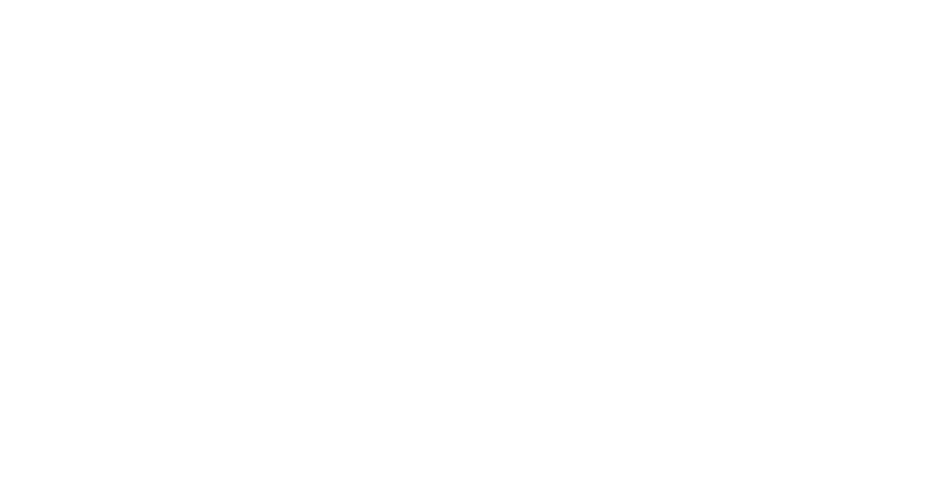
\includegraphics[width=12cm]{AcceleratorLattice-manual-logo.pdf} \\
\vskip 0.3in
\huge\bf David Sagan
\end{center}
}

\vfill
\break


%----------------------------------------------------------------

\cleardoublepage
\phantomsection 
\pdfbookmark[0]{Contents}{Contents}
\pdfbookmark[1]{Table of Contents}{toc} 
\tableofcontents

\cleardoublepage
\phantomsection 
\pdfbookmark[1]{List of Figures}{LoF} 
\listoffigures

\cleardoublepage
\phantomsection 
\pdfbookmark[1]{List of Tables}{LoT} 
\listoftables

%----------------------------------------------------------------
\setlength{\parskip}{\dPar}
\setlength{\parindent}{0ex}

%----------------------------------------------------------------
\part{Overview}
%----------------------------------------------------------------
\chapter{Introduction and Concepts}

%---------------------------------------------------------------------------
\section{Introduction}

This chapter is an introduction to, the \accellat package which is part of the
greater \scibmad ecosystem of toolkits and programs for accelerator simulations. With \accellat,
lattices can be constructed and manipulated. Essentially, a \vn{lattice} instance contains
a set of ``\vn{branches}'' and a branch contains 
an array of lattice \vn{elements} with each element representing an object like a magnet
or a RF cavity. A branch can be used to describe such
things as LINACs, storage rings, injection lines, X-ray beam lines, etc. Different branches in a
lattice can be connected together. For example, an injection line branch can be connected to a storage
ring branch or the lines of two rings can be connected together to form a colliding beam machine. 
This ability to describe the interconnections between branches means that 
a lattice instance can hold all the information about an entire machine complex from beam creation
to dump lines enabling a single lattice to be used as the basis of start-to-end simulations.

The sole purpose of the \accellat package is to implement methods for lattice construction.
Other stuff, like tracking and lattice analysis (for example, calculating
closed orbits and Twiss functions), is left to other packages in the \scibmad ecosystem.

%---------------------------------------------------------------------------
\section{Documentation}

There are three main sources of documentation of the \accellat package. 
One source is this PDF manual which gives in-depth documentationon. 
A second source is the web based introduction and overview guide.
Finally, functions, structs and other objects are documented in the code files themselves. 
Taking advantage of Julia's built-in documentation system, this code-file documentation 
can be accessed via using Julia's REPL.

%---------------------------------------------------------------------------
\section{Brief History}

\accellat has it's origins in the \bmad\cite{Sagan:Bmad2006} ecosystem of toolkits and programs 
developed over several decades at Cornell University.
While the development of \accellat is heavily influenced by the 
experience --- both good and bad --- of the development and use of \bmad as well as experience
with other accelerator simulation programs, the code of the two are
completely separate with \bmad being written in Fortran and \accellat being written in Julia.

The \julia language itself is used as the basis for constructing lattices with \accellat. 
Other simulation programs
have similarly utilized the underlying programming language for constructing 
lattices\cite{Appleby:Merlin2020,Iadarola:Xsuite2023}. This is in marked contrast to many accelerator
simulation programs such programs as MAD\cite{Grote:MAD1989}, Elegant\cite{Borland:Elegant2000}, and
Bmad. 
By using Julia for the lattice language, the user will automatically have access to such features 
as plotting, optimization packages, linear algebra packages, etc. 
This gives a massive boost to the versatility and usability of any \scibmad simulation program.
Moreover, maintainability is greatly enhanced due to the reduction in the amount of code that needs
to be developed.

%---------------------------------------------------------------------------------------------------
\section{Acknowledgements}

Thanks must go to the people who have contributed to this effort and without
whom \scibmad would only be a shadow of what it is today: 

\'Etienne Forest (aka Patrice Nishikawa),
Dan Abell,
Scott Berg,
Oleksii Beznosov,
Alexander Coxe,
Laurent Deniau,
Auralee Edelen,
Ryan Foussel,
Juan Pablo Gonzalez-Aguilera,
Georg Hoffstaetter,
Chris Mayes,
Matthew Signorelli,
Hugo Slepicka

%---------------------------------------------------------------------------
\section{Using AcceleratorLattice.jl}

\accellat is hosted on GitHub. The official repository is at
\begin{example}
  github.com/bmad-sim/AcceleratorLattice.jl
\end{example}
The \vn{README.md} file there has instructions on how to install \accellat.

A \vn{using} statement must be given before using \accellat in Julia
\begin{example}
  using AcceleratorLattice
\end{example}

%---------------------------------------------------------------------------
\section{Manual Conventions}
\label{s:manual.con}

This manual has the following conventions:
\begin{description}
%
\item[Type fields:]
\vn{Fields} of a type are also referred to as \vn{components} or \vn{parameters}.
A component \vn{c} of a type \vn{S} can be referred to as \vn{S.c}. In the case
of lattice elements, \vn{Ele} (the abstract type that all elements inherit from) is
used represent any of the subtypes such as \vn{Quadrupole}, etc. If the component
is an array, the notation \vn{S.c[]} can be used to emphasize this.
%
\end{description}

%---------------------------------------------------------------------------
\section{Lattice Elements}
\label{s:element.def}

The basic building block used to describe an accelerator is the lattice \vn{element}. An
element is generally something physical like a bending magnet or a
quadrupole, or a diffracting crystal. 

Lattice elements can be divided into two classes.
One class are the elements that particles are tracked through. These ``tracking'' elements are
contained in the ``tracking branches'' (\sref{s:branch.def}) of the lattice. Other elements, 
called ``\vn{lord}'' elements, are used to
represent relationships between elements. ``\vn{Super_lord}'' elements (\sref{c:super}) are
used when elements overlap spatially. ``\vn{Multipass_lord}'' elements (\ref{c:multipass})
are used when a beam goes through the same elements multiple times like in a recirculating Linac
or when different beam go through the same elements like in the interaction region of a
colliding beam machine.

%---------------------------------------------------------------------------
\section{Lattice Branches}
\label{s:branch.def}

The next level up from lattice \vn{elements} are the \vn{branches}.
Each branch holds an array of lattice elements. 
A branch is of type \vn{Branch}. 

There are two types of \vn{branches}: branches whose \vn{Branch.type} parameter is set to
a suitable subtype of \vn{LordBranch} holds Lord elements and 
branches whose \vn{Branch.type} parameter is set to \vn{TrackingBranch} holds an ordered
list of elements that can be tracked through. \accellat defines three lord branches named:
\begin{example}
  "super"       -- Contains super lord elements.
  "multipass"   -- Contains multipass lord elements.
  "girder"      -- Contains Girder elements.
\end{example}
Additional lord branches may be added by the user if desired.

A tracking branch can represent a LINAC, X-Ray beam line, storage ring, etc.
For all tracking branches, the first element in the element array
must be of type \vn{BeginningEle} (\sref{s:begin.ele}).
Additionally, for all tracking branches, 
the end element must be of type \vn{Marker} (\sref{s:mark}).

All tracking branches have a name \vn{Branch.name} inherited from the \vn{BeamLine} that defines
the branch in the lattice file and branches contains an array of elements \vn{Branch.ele[]}.
If the \vn{BeamLine} used to instantiate a tracking branch does not have a name, The default name
is used. The default name is \vn{"bN"} where \vn{N} is the index of the
branch in the \vn{Lattice.branch} array.

%---------------------------------------------------------------------------
\section{Lattices}
\label{s:lattice.def}

A \vn{lattice} (\sref{s:lattice.def}) is the root structure holding the information about a
``machine''. A machine may be as simple as a line of elements (like the elements of a Linac) or
as complicated as an entire accelerator complex with multiple storage rings, Linacs, transfer
lines, etc. All lattices are of type \vn{Lattice}.

Essentially, a \vn{lattice}, has an array \vn{Lattice.branch[]} of \vn{branches} with each branch 
describing part of the machine. 
Branches can be interconnected to form a unified whole.
Tracking branches can be interconnected using \vn{Fork} elements (\sref{s:fork}). 
This is used to simulate forking beam lines such as a connections to a transfer line, dump line, or an
X-ray beam line. The \vn{branch} from which other \vn{branches} fork but is not forked to by any
other \vn{branch} is called a \vn{root} branch.

A lattice may contain multiple \vn{root} \vn{branches}. For example, a pair of intersecting storage
rings will generally have two \vn{root} branches, one for each ring.

Branches can be accessed by name using the overloaded index operator for \vn{Lattice}. 
For example, if \vn{lat} is an instance of a lattice, the super lord branch (\sref{s:branch.def}),
which has the name \vn{"super"}, can be accessed via:
\begin{example}
  lat["super"]     # Access by branch name
  lat.branch[2]    # Access by branch index
\end{example}
Where it is assumed for this example that the super lord branch has index 2.

Similarly, lattice elements can be accessed by name or by index.
For example, if \vn{lat} is a lattice instance, and \vn{"q1"} is the name of an element or
elements that are in a branch named "b2", the following are equivalent:
\begin{example}
  elist = lat["q1"]
  elist = find(lat, "q1")
  b2 = lat.branch["b2"]; elist = b2["q1"]
\end{example}
\vn{elist} will be a vector of elements since a name may match to multiple elements.

%---------------------------------------------------------------------------
\section{AcceleratorLattice Conventions}
\label{s:conventions}

\accellat has the following conventions:
\begin{description}
%
\item[Evaluation is at upstream end:] 
For lattice element parameters that are s-dependent, the evaluation location is the
\vn{upstream} edge of the element (\sref{s:ref.construct}). These parameters include the 
element's floor position, the reference energy/momentum, and the s-position.
%
\end{description}

%---------------------------------------------------------------------------
\section{Minimal Working Lattice Example}
\label{s:min.lat}

The following is a minimal example of constructing a lattice with a quadrupole, drift, and then
a bend:
\begin{example}
  using AcceleratorLattice
  @ele begin_ele = BeginningEle(pc_ref = 1e7, species_ref = species("electron"))
  @ele q = Quadrupole(L = 0.6, K2 = 0.3)
  @ele d = Drift(L = 0.4)
  @ele b = Bend(L = 1.2, angle = 0.001)

  a_line = beamline("simple_line", [begin_ele, q, d, b])
  lat = Lattice("simple_lat", [a_line])
\end{example}

%---------------------------------------------------------------------------
\section{Differences From Bmad}

There are many differences between \accellat and \bmad. Many of of these will be fairly
obvious. Some differences to be aware of:
\begin{description}
\item
\bmad is generally case insensitive (except for things like file names). \accellat, like
the Julia language, is case sensitive.
%
With \bmad, the branch array within a lattice and the element array within a branch is
indexed from zero. With \scibmad, indexing of \vn{Lattice.branch[]} and \vn{branch.ele[]} is 
from one conforming to the Julia standard.
%
\item
The \bmad names for the coordinate systems (\sref{s:coords}) was somewhat different and not
always consistent. The \vn{floor} and \vn{element body} names are the same but \vn{machine}
coordinates are called the \vn{laboratory} in \bmad.
%
\item
Evaluation was at the downstream end (\sref{s:conventions}) in \bmad not the upstream end.
%
\item
With \bmad a value for any aperture limits of zero means the limit does not exist.
with \accellat a value of \vn{NaN} means the aperture does not exist. Additionally, with
\bmad a positive value for \vn{x1_limit} or \vn{y1_limit} meant that the aperture was
on the negative side of the \vn{x-axis} or \vn{y-axis} respectively. With \accellat, a positive
value for \vn{x_limit[1]} or \vn{y_limit[1]} means the aperture is on the positive side of 
of the \vn{x-axis} or \vn{y-axis} respectively. This makes the notation consistent across 
the different ways to specify apertures (compare with \vn{Mask} element syntax.).
%
\item
\accellat defines the reference point for misalignment of a Bend element as the center 
of the chord between the entrance and exit end points. 
With \bmad, the reference point is at the center of the reference trajectory arc between the entrance
and the exit. An additional difference is that the \bmad \vn{roll} misalignment is called \vn{tilt}
under \accellat.
%
\item
\bmad does not allow redefinition of named variables nor elements. \accellat allows this.
%
\item
With \bmad, the beginning and end elements are implicitly inserted into a branch line.
With \accellat, only an end element will be implicitly inserted if the end of the beamline is
not a marker. 
Also with \bmad the beginning element is always named \vn{Beginning} while with \accellat there
is no restriction on the name. 
%
\item
Restrictions on the order of statements used to create a lattice are different. 
For example, in \bmad, a statement defining a lattice element can be placed anywhere
except if there is an \vn{expand_lattice} statement and the element is not being used
with superposition in which case the element definition must be before the \vn{expand_lattice}
statement. With \accellat, element definitions must come before the element is used in a line.
%
\item
With \bmad superposition of two non-drift elements, if there existed the appropriate
combined type, will result in a \vn{super_slave} of the appropriate combined type. For example,
a \vn{solenoid} superimposed over a \vn{quadrupole} would give a \vn{sol_quad} \vn{super_slave} with
\vn{solenoid} and \vn{quadrupole} \vn{super_lords}. The problem here is that calculation of the
\vn{super_slave} parameters may not be possible. For example if the \vn{super_lord}
elements are misaligned, in general it is not possible to compute a corresponding \vn{super_slave}
misalignment. To avoid this, \accellat creates a \vn{UnionEle} \vn{super_slave} element
(which in \bmad is known as a ``jumbo'' \vn{super_slave}). It is up to the tracking routines to
figure out how to track though a \vn{UnionEle}
%
\item
In \vn{Bmad} there are two types of bends called \vn{sbend} and \vn{rbend}. 
This organization was inherited from \vn{MAD}. While both \vn{sbends} and \vn{rbends}
represent the same physical type of bend, the two have different ways to specify the bend parameters. 
This can be confusing since \vn{rbends} and \vn{sbends} use the same names for different parameters.
For example, the length \vn{l} for an \vn{sbend} is the arc length but for an \vn{rbend} it is the
chord length. To avoid confusion, \accellat combines the two into a single \vn{Bend} type with
distinct parameter names. For example, \vn{L} is the arc length and \vn{L_chord} is the chord length.
\end{description}




\chapter{Orientation}
\label{c:orient}

\section{What is Bmad?}

\bmad is an open-source software envionment for simulating charged particles and
X-rays. \bmad is not a program itself but is used by programs for doing calculations. The advantage
of \bmad over a stand-alone simulation program is that when new types of simulations need to be
developed, \bmad can be used to cut down on the time needed to develop such programs with the added
benefit that the number of programming errors will be reduced.

Over the years, \bmad has been used for a wide range of charged-particle and X-ray simulations. This
includes:
\begin{example}
Lattice design                                  X-ray simulations
Spin tracking                                   Wakefields and HOMs
Beam breakup (BBU) simulations in ERLs          Touschek Simulations
Intra-beam scattering (IBS) simulations         Dark current tracking
Coherent Synchrotron Radiation (CSR)            Frequency map analysis
\end{example}

%---------------------------------------------------------------------------
\section{Resources: More Documentation, Obtaining Bmad, etc.}
\label{s:bmad.web}

More information and download instructions are readily available on GitHub:
\begin{example}
  \url{\detokenize{https://github.com/bmad-sim}}
\end{example}

\chapter{Concepts and Organization}
\label{c:lat.concepts}

This chapter is an overview of some of the nomenclature used by \bmad. Presented are the basic
concepts, such as \vn{element}, \vn{branch}, and \vn{lattice} that \bmad uses to describe such
things as LINACs, storage rings, X-ray beam lines, etc.

%---------------------------------------------------------------------------
\section{Lattice Elements}
\label{s:element.def}

The basic building block used to describe a machine is the \vn{lattice} \vn{element}. An
element can be a physical thing that particles travel ``through'' like a bending magnet, a
quadrupole or a Bragg crystal, or something like a \vn{marker} element (\sref{s:mark}) that is used
to mark a particular point in the machine.  Besides physical elements, there are \vn{controller}
elements (\sref{??}) that can be used for parameter control of other elements.

Chapter~\sref{c:elements} lists the complete set of different element types that \bmad knows about.

In a lattice \vn{branch} (\sref{s:branch.def}), The ordered array of elements are assigned an 
\vn{ element index}
starting from one. The first element is called \vn{beginning_ele} (\sref{s:begin.ele}).
This element is always included in every \vn{branch} \sref{s:branch.def} and is used as a
marker for the beginning of the \vn{branch}.  Additionally, every branch will have a final
marker element (\sref{s:mark}) named \vn{end_ele}.

%---------------------------------------------------------------------------
\section{Lattice Branches}
\label{s:branch.def}

The next level up from a \vn{element} is the \vn{branch}. A 
\vn{branch} contains an ordered sequence of lattice elements that a particle will travel through. A
branch can represent a LINAC, X-Ray beam line, storage ring or anything else that can be represented
as a simple ordered list of elements.

Chapter~\sref{c:sequence} shows how a \vn{branch} can be defined using \vn{line}s.

Branches can be interconnected using \vn{fork} elements (\sref{s:fork}). This
is used to simulate forking beam lines such as a connections to a transfer line, dump line, or an
X-ray beam line. A \vn{branch} from which other \vn{branches} fork but is not forked to by any
other \vn{branch} is called a \vn{root} branch. A branch that is forked to by some other branch
is called a \vn{downstream} branch.

There are two types of \vn{branches}: \vn{LordBranches} and \vn{TrackingBranches}, Branches whose \vn{Branch.type} are set to \vn{LordBranch}
hol

%---------------------------------------------------------------------------
\section{Lattice}
\label{s:lattice.def}

A \vn{lattice} (\sref{s:lattice.def}), has an array of \vn{branches}. Each \vn{branch} in this array
has a name an is assigned an index starting from one. 
Additionally, each \vn{branch} is assigned a name which is the
\vn{line} that defines the branch (\sref{s:use}).

A \vn{lattice} contains an array of \vn{branches} that can be interconnected together to describe an entire machine
complex. A \vn{lattice} can include such things as transfer lines, dump lines, x-ray beam lines,
colliding beam storage rings, etc. All of which can be connected together to form a coherent whole. In
addition, a lattice may contain \vn{controller elements} (Table~\ref{t:control.classes}) which can
simulate such things as magnet power supplies and lattice element mechanical support structures.

Branches can be interconnected using \vn{fork} and \vn{photon_fork} elements (\sref{s:fork}). This
is used to simulate forking beam lines such as a connections to a transfer line, dump line, or an
X-ray beam line. The \vn{branch} from which other \vn{branches} fork but is not forked to by any
other \vn{branch} is called a \vn{root} branch.

A lattice may contain multiple \vn{root} \vn{branches}. For example, a pair of intersecting storage
rings will generally have two \vn{root} branches, one for each ring. The \vn{use} statement
(\sref{s:use}) in a lattice file will list the \vn{root} \vn{branches} of a lattice. To connect
together lattice elements that are physically shared between branches, for example, the interaction
region in colliding beam machines, \vn{multipass} lines (\sref{s:multipass}) can be used.

The root branches of a lattice are defined by the \vn{use} (\sref{s:use}) statement. To further
define such things as dump lines, x-ray beam lines, transfer lines, etc., that branch off from a
root branch, a forking element is used.  \vn{Fork} elements can define where the particle beam can
branch off, say to a beam dump. \vn{photon_fork} elements can define the source point for X-ray
beams.  Example:
\begin{example}
  erl: line = (..., dump, ...)               ! Define the root branch 
  use, erl
  dump: fork, to_line = d_line               ! Define the fork point
  d_line: line = (..., q3d, ...)             ! Define the branch line
\end{example}

Like the root branch \bmad always automatically creates an element with \vn{element index} 0 at the
beginning of each branch called \vn{beginning}. The longitudinal \vn{s} position of an element in a
branch is determined by the distance from the beginning of the branch.

Branches are named after the line that defines the \vn{branch}. In the above example, the branch
line would be named \vn{d_line}. The root branch, by default, is called after the name in the
\vn{use} statement (\sref{s:use}).

The ``branch qualified'' name of an element is of the form
\begin{example}
  branch_name>>element_name
\end{example}
where \vn{branch_name} is the name of the branch and \vn{element_name} is the ``regular'' name of
the element. Example:
\begin{example}
  root>>q10w
  xline>>cryst3
\end{example}
When parsing a lattice file, branches are not formed until the lattice is expanded
(\sref{s:expand}). Therefore, an \vn{expand_lattice} statement is required before branch qualified
names can be used in statements. See \sref{s:ele.match} for more details.

%---------------------------------------------------------------------------
\section{Lord and Slave Elements}
\label{s:lord.slave}

\begin{figure}[tb]
 \begin{center}
 \includegraphics[width=6.0in]{superimpose-ip.pdf}
 \caption[Superposition example.]{
Superposition Example. A) Interaction region layout with quadrupoles overlapping a solenoid. B) The
Bmad lattice representation has a list of split elements to track through and the undivided ``lord''
elements. Pointers (double headed arrows), keep track of the correspondence between the lords and
their slaves.
 }
 \label{f:super.ip}
 \end{center}
 \end{figure}

%---------------------------------------------------------------------------

A real machine is more than a collection of independent lattice elements. For example, the field
strength in a string of elements may be tied together via a common power supply, or the fields of
different elements may overlap.

\bmad tries to capture these interdependencies using what are referred to as \vn{lord} and
\vn{slave} elements. The \vn{lord} elements may be divided into two classes. In one class are the
\vn{controller} elements.  These are \vn{overlay} (\sref{s:overlay}), \vn{group} (\sref{s:group}),
\vn{ramper} (\sref{s:ramper}), and \vn{girder} (\sref{s:girder}) elements that control the
attributes of other elements which are their slaves.

The other class of \vn{lord} elements embody the separation of the physical element from the track
that a particle takes when it passes through the element. There are two types

An example will make this clear.  \vn{Superposition} (\sref{s:super}) is the ability to overlap
lattice elements spatially. \fig{f:super.ip} shows an example which is a greatly simplified version
of the IR region of Cornell's CESR storage ring when CESR was an e+/e-- collider. As shown in
\fig{f:super.ip}A, two quadrupoles named \vn{q1w} and \vn{q1e} are partially inside and partially
outside the interaction region solenoid named \vn{cleo}. In the lattice file, the IR region layout
is defined to be
 {\small
\begin{example}
  cesr: line = (... q1e, dft1, ip, dft1, q1w ...)
  cleo: solenoid, l = 3.51, superimpose, ref = ip
\end{example}
 }
The line named \vn{cesr} ignores the solenoid and just contains the interaction point marker element
named \vn{ip} which is surrounded by two drifts named \vn{dft1} which are, in turn, surrounded by
the \vn{q1w} and \vn{q1e} quadrupoles. The solenoid is added to the layout on the second line by
using superposition. The ``ref = ip'' indicates that the solenoid is placed relative to \vn{ip}. The
default, which is used here, is to place the center of the superimposed \vn{cleo} element at the
center of the \vn{ip} reference element.  The representation of the lattice in \bmad will contain
two branch \vn{sections} (``sections'' is explained more fully later): One section, called the
\vn{tracking section}, contains the elements that are needed for tracking particles. In the current
example, as shown in \fig{f:super.ip}B, the first IR element in the tracking section is a quadrupole
that represents the part of \vn{q1e} outside of the solenoid. The next element is a combination
solenoid/quadrupole, called a \vn{sol_quad}, that represents the part of \vn{q1e} inside \vn{cleo},
etc.  The other branch section that Bmad creates is called the \vn{lord section} This section
contain the undivided ``physical'' \vn{super_lord} elements (\sref{s:super}) which, in this case are
\vn{q1e}, \vn{q1w}, and \vn{cleo}. Pointers are created between the lords and their \vn{super_slave}
elements in the tracking section so that changes in parameters of the lord elements can be
transferred to their corresponding slaves.

\vn{super_lord}s are used when there are overlapping fields between elements, the other case where
there is a separation between the physical (lord) element and the (slave) element(s) used to track
particles through comes when a particle passes through the same physical element multiple times such
as in an Energy Recovery Linac or where different beams pass through the same element such as in an
interaction region. In this case, \vn{multipass_lords} representing the physical elements and
\vn{multipass_slaves} elements which are used for tracking can be defined (\sref{s:multipass}).
Superposition and multipass can be combined in situations where there are overlapping fields in
elements where the particle passes through

Each lattice element is assigned a \vn{slave_status} indicating what kind of slave it is and a
\vn{lord_status} indicating what kind of lord it is. Normally a user does not have to worry about
this since these status attributes are handled automatically by \bmad.  The possible
\vn{lord_status} settings are:
  \begin{description}
  \item[girder_lord]\Newline 
A \vn{girder_lord} element is a \vn{girder} element  (\sref{s:girder}). 
  \item[multipass_lord]\Newline
\vn{multipass_lord} elements are created when
multipass lines are present (\sref{s:multipass}). 
  \item[overlay_lord]\Newline 
An \vn{overlay_lord} is an \vn{overlay} element (\sref{s:overlay}). 
  \item[group_lord]\Newline 
A \vn{group_lord} is a \vn{group} element (\sref{s:group}).
  \item[super_lord]\Newline 
A \vn{super_lord} element is created when elements are
superimposed on top of other elements (\sref{s:super}).
  \item[not_a_lord]\Newline
This element does not control anything.
  \end{description}
Any element whose \vn{lord_status} is something other than
\vn{not_a_lord} is called a \vn{lord} element. In the \vn{tracking part}
of the branch, \vn{lord_status} will always be
\vn{not_a_lord}. In the \vn{lord section} of the branch, under normal
circumstances, there will never be any \vn{not_a_lord} elements.

Lord elements are divided into two classes.  A \vn{major} lord represents a physical element which
the slave elements are a part of.  \vn{super_lord}s and \vn{multipass_lord}s are \vn{major} lords.
As a consequence, a \vn{major} lord is a lord that controls nearly all of the attributes of its
slaves.  The other lords --- \vn{girder_lord}s, \vn{group_lord}s and \vn{overlay_lord}s --- are
called \vn{minor} lords.  These lords only control some subset of a slaves attributes.

The possible \vn{slave_status} settings are
  \begin{description}
  \item[multipass_slave]\Newline
A \vn{multipass_slave} element is the slave of a \vn{multipass_lord}
(\sref{s:multipass}).
  \item[slice_slave]\Newline
A \vn{slice_slave} element represents a longitudinal slice of another element.
Slice elements are not part of the lattice but rather are created on-the-fly
when, for example, a program needs to track part way through an element.
  \item[super_slave]\Newline 
A \vn{super_slave} element is an element in the tracking part of the branch that 
has one or more \vn{super_lord} lords (\sref{s:super}).
  \item[minor_slave]\Newline
\vn{minor_slave} elements are elements that are not \vn{slice_slave}s and are only controlled
by \vn{minor} lords (\vn{overlay_lord}s, \vn{group_lord}s, or \vn{girder_lord}s).
  \item[free]\Newline
A \vn{free} element is an element with no lords.
  \end{description}

For historical reasons, each \vn{branch} in a lattice has a \vn{tracking section} and a \vn{lord
section} and the \vn{tracking section} is always the first (lower) part of the element array and the
\vn{lord section} inhabits the second (upper) part of the array.  All the \vn{lord} elements are put
in the \vn{lord section} of branch 0 and all the other \vn{lord sections} of all the other branches
are empty.

As a side note, \'Etienne Forest's PTC code (\sref{s:ptc.intro}) uses separate structures to
separate the physical element, which PTC calls an \vn{element} from the particle track which PTC
call a \vn{fibre}.  [Actually, PTC has two structures for the physical element, \vn{element} and
\vn{elementp}. The latter being the ``polymorph'' version.] This \vn{element} and \vn{fibre}
combination corresponds to \bmad \vn{multipass_lord} and \vn{multipass_slave} elements. PTC does not
handle overlapping fields as \bmad does with \vn{superposition} (\sref{s:super}).



%----------------------------------------------------------------
\part{AcceleratorLattice.jl: Lattice Construction and Manipulation}
%----------------------------------------------------------------
\chapter{Constructing a Lattice}
\label{c:construct-lat}

%---------------------------------------------------------------------------------------------------
\section{Switches}
\label{s:switch}

A \vn{switch} is like an enumerated value except that 


A \vn{switch} is a switch category identifier name, conventionally with the word \vn{Switch} at the end, 
with a set of possible values. Switches are like enums without the associated integer. 
The advantage of switches is that a given switch value can be used for different switch groups. 

For example, 

How to create switches...





%---------------------------------------------------------------------------------------------------
\section{Defining a Lattice Element}
\label{s:ele.def}

The \julia language itself is used as the basis for constructing lattices. Other simulation programs
have similarly utilized the underlying programming language for constructing lattices\cite{merlin++,xsuite},
but this is in marked contrast to such programs as MAD\cite{mad}, Elegant\cite{elegant}, and the 
original \bmad\cite{bmad-orig}. 

Chapter~\sref{c:ele} gives a list of elements defined by \Bmad. Elements are defined using the \vn{@ele}
macro. The general syntax is:
\begin{example}
  @ele eleName = eleType(param1 = val1, param2 = val2, ...)
\end{example}
where \vn{eleName} is the name of the element, \vn{eleType} is the type of element, \vn{param1}, \vn{param2},
etc. are parameter names and \vn{val1}, \vn{val2}, etc. are the parameter values.
Example:
\begin{example}
  @ele qf = Quadrupole(len = 0.6, K1 = 0.370)
\end{example}
The \vn{@ele} macro will construct a \julia variable with the name \vn{eleName}. Additionally the element
that this variable references will also hold \vn{eleName} as the name of the element.

To copy an element use the \vn{deepcopy} constructor.

%---------------------------------------------------------------------------------------------------
\section{Defining a Lattice Element Type}
\label{s:ele.type}

All lattice element types like \vn{Quadrupole}, \vn{Marker}, etc. are subtypes of the abstract type
\vn{Ele}. To construct a new type, use the \vn{\@construct_ele_type} macro. Example:
\begin{example}
  @construct_ele_type MyEleType
\end{example}

%---------------------------------------------------------------------------------------------------
\section{Lattice Element Internals}
\label{s:ele.inside}

All element types have a single component called \vn{pdict} (``parameter dict'') which is of
type \vn{Dict\{Symbol,Any\}}. Using a \vn{Dict} has advantages and disadvantages. The advantage is
that an element is not restricted as to what can be stored in it. The disadvantage is that it is not
type stable (\sref{s:type.stable}). This is generally acceptable when lattices are constructed but
is undesirable during tracking. To regain type stability during tracking, element parameters are
put into immutable structs called \vn{element parameter} groups 
and these structs are stored in \vn{pdict}. During tracking, the tracking
code can access element parameters via the struct which makes the code type stable as will be illustrated below.

The \vn{element parameter} group structures are all subtypes of the abstract type \vn{EleParameterGroup}.
For example, the \vn{LengthGroup} holds the length and s-positions of the element:
\begin{example}
  @kwdef struct LengthGroup <: EleParameterGroup
    L::Float64 = 0
    s::Float64 = 0
    s_downstream::Float64 = 0
  end
\end{example}
The \vn{\@kwdef} macro automatically defines a keyword-based constructor for \vn{LengthGroup}. 
When a parameter group is stored in an element's \vn{pdict}, the key will be the symbol associated
with the struct which in this case is \vn{:LengthGroup}. For example, an element's length can be
accessed via \vn{ele.pdict[:LengthGroup].L}. 


\etcetc...





\chapter{Lattice Elements}
\label{c:elements}
\index{element|hyperbf}

%---------------------------------------------------------------------------------------------------

A lattice is made up of a collection of elements --- quadrupoles,
bends, etc. This chapter discusses the various types of elements
available in \bmad.

\begin{table}[htb]
\centering
{\tt
\begin{tabular}{llll} \toprule
  {\it Element}     & {\it Section}         & {\it Element}      & {\it Section}      \\ \midrule
                                            &  Match             & \ref{s:match}      \\
  AC_Kicker         & \ref{s:ac.kick}       &  Monitor           & \ref{s:monitor}    \\
  BeamBeam          & \ref{s:beambeam}      &  Multipole         & \ref{s:mult}       \\
  Beginning_Ele     & \ref{s:begin.ele}     &  Null_Ele          & \ref{s:null.ele}   \\
  Converter         & \ref{s:converter}     &  Octupole          & \ref{s:oct}        \\
  Crab_Cavity       & \ref{s:crab}          &  Patch             & \ref{s:patch}      \\
  Custom            & \ref{s:custom}        &  Photon_Fork       & \ref{s:fork}       \\
  Drift             & \ref{s:drift}         &  Pipe              & \ref{s:monitor}    \\
  E_Gun             & \ref{s:e.gun}         &  Quadrupole        & \ref{s:quad}       \\
  Ecollimator       & \ref{s:col}           &  Rbend             & \ref{s:bend}       \\
  ElSeparator       & \ref{s:elsep}         &  Rcollimator       & \ref{s:col}        \\
  EM_Field          & \ref{s:em.field}      &  RF_bend           & \ref{s:rf.bend}    \\
  Fiducial          & \ref{s:fiducial}      &  RFcavity          & \ref{s:rfcav}      \\
  Floor_Shift       & \ref{s:floor.ele}     &  Sad_Mult          & \ref{s:sad.mult}   \\
  Foil              & \ref{s:foil}          &  Sbend             & \ref{s:bend}       \\
  Fork              & \ref{s:fork}          &  Sextupole         & \ref{s:sex}        \\
  GKicker           & \ref{s:gkicker}       &  Sol_Quad          & \ref{s:sq}         \\
  HKicker           & \ref{s:hvkicker}      &  Solenoid          & \ref{s:sol}        \\
  Hybrid            & \ref{s:hybrid}        &  Taylor            & \ref{s:taylor}     \\
  Instrument        & \ref{s:monitor}       &  Thick_Multipole   & \ref{s:thick.mult} \\
  Kicker            & \ref{s:kicker}        &  Undulator         & \ref{s:wiggler}    \\
  Lcavity           & \ref{s:lcav}          &  VKicker           & \ref{s:hvkicker}   \\ 
  Marker            & \ref{s:mark}          &  Wiggler           & \ref{s:wiggler}    \\
  Mask              & \ref{s:mask}          &                    &                    \\
  \bottomrule
\end{tabular}
} \caption{Table of element types suitable for use with charged particles. Also see
Table~\ref{t:control.classes}} \label{t:particle.classes}
\end{table}

\index{MAD}
Most element types available in \mad are provided in \bmad.  Additionally, \bmad provides a number
of element types that are not available in \mad.  A word of caution: In some cases where both \mad
and \bmad provide the same element type, there will be an overlap of the attributes available but
the two sets of attributes will not be the same.  The list of element types known to \bmad is shown
in Table~\ref{t:particle.classes}, \ref{t:photon.classes}, and \ref{t:control.classes}.
Table~\ref{t:particle.classes} lists the elements suitable for use with charged particles,
Table~\ref{t:photon.classes} which lists the elements suitable for use with photons, and finally
Table~\ref{t:control.classes} lists the \vn{controller} element types that can be used for parameter
control of other elements. Note that some element types are suitable for both particle and photon
use.

\begin{table}[ht]
\centering
{\tt
\begin{tabular}{llll} \toprule
  {\it Element}      & {\it Section}         & {\it Element}         & {\it Section}       \\ \midrule
  Beginning_Ele      & \ref{s:begin.ele}     &    Lens               & \ref{s:lens}        \\
  Capillary          & \ref{s:capillary}     &  Marker               & \ref{s:mark}        \\
  Crystal            & \ref{s:crystal}       &  Mask                 & \ref{s:mask}        \\
  Custom             & \ref{s:custom}        &  Match                & \ref{s:match}       \\
  Detector           & \ref{s:detector}      &  Monitor              & \ref{s:monitor}     \\ 
  Diffraction_Plate  & \ref{s:diff.plate}    &  Mirror               & \ref{s:mirror}      \\
  Drift              & \ref{s:drift}         &  Multilayer_Mirror    & \ref{s:multilayer}  \\
  Ecollimator        & \ref{s:col}           &  Patch                & \ref{s:patch}       \\
  Fiducial           & \ref{s:fiducial}      &  Photon_Fork          & \ref{s:fork}        \\
  Floor_Shift        & \ref{s:floor.ele}     &  Photon_Init          & \ref{s:photon.init} \\
  Fork               & \ref{s:fork}          &  Pipe                 & \ref{s:monitor}     \\
  GKicker            & \ref{s:gkicker}       &  Rcollimator          & \ref{s:col}         \\
  Instrument         & \ref{s:monitor}       &  Sample               & \ref{s:sample}      \\
  \bottomrule
\end{tabular}
}
\caption{Table of element types suitable for use with photons. Also see Table~\ref{t:control.classes}}
\label{t:photon.classes}
\end{table}

\begin{table}[ht]
\centering
{\tt
\begin{tabular}{llll} \toprule
  {\it Element}  & {\it Section}     & {\it Element}  & {\it Section}    \\ \midrule
  Group          & \ref{s:group}     &  Overlay       & \ref{s:overlay}  \\
  Girder         & \ref{s:girder}    &  Ramper        & \ref{s:ramper}   \\ \bottomrule
\end{tabular}
}
\caption{Table of controller elements.}
\label{t:control.classes}
\end{table}

For a listing of element attributes for each type of element, see Chapter~\sref{c:attrib.list}.

\newpage

%---------------------------------------------------------------------------------------------------
\section{Lattice Element Parameters}

Before discussing lattice elements themselves, the element parameters need to be discussed first.
Element parameters are divided into immutable struct groups which inherit from the abstract type
\vn{EleParameterGroup}. The parameter groups are:
\begin{example}
\end{example}

For example, the position of the element with respect

Element parameters are listed in 

%---------------------------------------------------------------------------------------------------
\section{Anatomy of a Lattice Element}

All lattice elements inherit from the abstract type \vn{Ele}. There is a macro \vn{construct_ele_type}
that is used to construct a new type of element. For example:
\begin{example}
  @construct_ele_type Bend
\end{example}
this defines the immutable \vn{Bend} struct which inherits from \vn{Ele}. 

All element structs have a single \vn{Dict\{Symbol,Any\}} field called \vn{param}.
The dot selection operator has been overloaded so that something like \vn{ele.name}
is mapped to \vn{ele.param[:name]}. Except!


%---------------------------------------------------------------------------------------------------
\section{AC_Kicker}
\label{s:ac.kick}
\index{ab_kicker|hyperbf}

An \vn{ac_kicker} element simulates a time dependent kicker element.

General \vn{ac_kicker} attributes are:
\begin{center}
\tt
\begin{tabular}{llll} \toprule
  {\sl Attribute Class}      & Section           & {\sl Attribute Class}      & Section         \\ \midrule
  Aperture limits            & \ref{s:limit}     & Is_on                      & \ref{s:is.on}   \\
  Chamber wall               & \ref{s:wall}      & Length                     & \ref{s:l}       \\
  Custom Attributes          & \ref{s:cust.att}  & Mag \& Elec multipoles     & \ref{s:multip}  \\
  Description strings        & \ref{s:alias}     & Offsets, pitches \& tilt   & \ref{s:offset}  \\
  Field Maps                 & \ref{s:fieldmap}  & Reference energy           & \ref{s:energy}  \\ 
  Fringe Fields              & \ref{s:fringe}    & Superposition              & \ref{s:super}   \\
  Hkick \& Vkick             & \ref{s:kick}      & Symplectify                & \ref{s:symp}    \\
  Integration settings       & \ref{s:integ}     & Tracking \& transfer map   & \ref{c:methods} \\
  \bottomrule
\end{tabular}
\end{center}
\toffset
See \sref{s:list.ac.kicker} for a full list of element attributes along with a their units.

Attributes specific to a \vn{ac_kicker} element are:
\begin{example}
  t_offset        = <Real>              ! Time offset of field waveform.
  interpolation   = <switch>            ! cubic (default) or linear.
  amp_vs_time = \{(<time1>, <Amp1>), (<time2>, <Amp2>), ...\}  ! Field amp vs Time.
  frequencies = \{(<freq1>, <Amp1>, <phi1>), 
                              (<freq2>, <Amp2>, <phi2>), ...\} ! Freq components.
\end{example}
Note: The \vn{frequencies} attribute phases \vn{phi1}, \vn{phi2}, \vn{phi3}, etc., have units of
\vn{radians/2pi}.

An \vn{ac_kicker} element is like a \vn{kicker} (\sref{s:kicker}) element except that the field
varies in time. The field is calculated in two steps:
\begin{enumerate}
\item Calculate the field the same as for a \vn{kicker} element (\sref{s:kicker}).
\item Scale the field using the function $A(\delta t)$ (discussed below)
\begin{equation}
  B(\delta t) = A(\delta t) \, B_0, \qquad E(\delta t) = A(\delta t) \, E_0
\end{equation}
where $B$ and $E$ are the applied magnetic and electric fields, and $B_0$ and $E_0$ are the fields
as calculated as if the element where a \vn{kicker} ignoring the time dependence.
\end{enumerate}

$\delta t = t_{eff} - t_0$ where $t_{eff}$ is the effective time as discussed in \sref{s:rf.time}
and $t_0$ is the value of the \vn{t_offset} attribute.

There are two ways to specify the dimensionless time variation $A(\delta t)$ of the field. One way
is to specify points $(A, \delta t)$ using the \vn{amp_vs_time} attribute. Example:
\begin{example}
  mk: ac_kicker, l = 0.3, scale_multipoles = F, b1 = 0.27, t_offset = 3.6e-8,
          amp_vs_time = \{(-1.2e-6, 0.02), ... \} 
\end{example}
The element in this example is an AC quadrupole kicker. The times (in seconds) must be in ascending
order and no two times may be the same. The method used to interpolate between the time points is
determined by the setting of the \vn{interpolate} parameter which may be one of
\begin{example}
  linear      ! Linear interpolation.
  cubic       ! Cubic spline interpolation (default).
\end{example}
For times outside of the range specified by \vn{amp_vs_time}, the amplitude will be extrapolated.
For the cubic spline, extrapolation is only permitted over a distance outside the time range equal
to the time difference between an end point and the next nearest point.

The second way to specify the waveform is to specify the frequencies in the spectrum using the
\vn{frequencies} attribute. In this case the amplitude is:
\begin{equation}
  A(t) = \sum_i \, A_i \, \cos( 2 \, \pi (f_i \, \delta t + \phi_i))
\end{equation}
Example:
\begin{example}
  mk: ac_kicker, l = 0.3, field_calc = fieldmap, cartesian_map = \{...\},
          frequencies = \{(3.4e6, 0.34, 0.12), ...\}, a0_elec = 1e5
\end{example}
When using a frequency spectrum, the \vn{interpolate} attribute is ignored. Note: The units of the
phases \vn{phi} with the \vn{frequencies} attribute are \vn{rad/2pi}.

To specify an \vn{amp_vs_time} component after an \vn{ac_kicker} element has been defined, use the
syntax
\begin{example}
  name[AMP_VS_TIME(i)%time]      ! Time of i^th point.
  name[AMP_VS_TIME(i)%amp]       ! Amplitude of i^th point.
\end{example}
where \vn{name} is the name of the element and \vn{i} is the index of the point.
To specify a \vn{frequencies} component after an \vn{ac_kicker} element has been defined, use the
syntax
\begin{example}
  name[FREQUENCIES(i)%freq]     ! Frequency of i^th spectrum point.
  name[FREQUENCIES(i)%amp]      ! Amplitude of i^th spectrum point.
  name[FREQUENCIES(i)%phi]      ! Phase (rad/2pi) of i^th spectrum point.
\end{example}
Example:
\begin{example}
  mk: ac_kicker, amp_vs_time = \{(-1.2e-6, 0.02), ... \} 
  mk[amp_vs_time(2)%amp] = 0.03  ! Change 2nd point amplitude.
\end{example}

When specifying the time dependent using a set of frequencies, it is generally advisable to use
absolute time tracking (\sref{s:rf.time}). This can be done in the lattice file by setting
\begin{example}
  bmad_com[absolute_time_tracking] = T
\end{example}

Note: The calculated field will only obey Maxwell's equations in the limit that the time variation
of the field is ``slow'':
\begin{equation}
  \omega \ll \frac{c}{r}
\end{equation}
where $\omega$ is the characteristic frequency of the field variation, $c$ is the speed of light,
and $r$ is the characteristic size of the \vn{ac_kicker} element. That is, the fields at opposite
ends of the element must be able to ``communicate'' (which happens at the speed of light) in a time
scale short compared to the time scale of the change in the field.

\newpage

%-----------------------------------------------------------------
\section{BeamBeam}
\label{s:beambeam}
\index{beambeam|hyperbf}

A \vn{beambeam} element simulates an interaction with an opposing
(``strong'') beam traveling in the opposite direction. The strong beam
is assumed to be Gaussian in shape. In the \vn{bmad_standard}
calculation the beam--beam kick is computed using the
Bassetti--Erskine complex error function formula\cite{b:talman}

General \vn{beambeam} attributes are:
\begin{center} 
\tt
\begin{tabular}{llll} \toprule
  {\sl Attribute Class}      & Section          & {\sl Attribute Class}      & Section         \\ \midrule
  Aperture limits            & \ref{s:limit}    & Is_on                      & \ref{s:is.on}   \\
  Chamber wall               & \ref{s:wall}     & Offsets, pitches \& tilt   & \ref{s:offset}  \\
  Custom Attributes          & \ref{s:cust.att} & Reference energy           & \ref{s:energy}  \\
  Description strings        & \ref{s:alias}    & Superposition              & \ref{s:super}   \\
  Is_on                      & \ref{s:is.on}    & Tracking \& transfer map   & \ref{c:methods} \\ 
  \bottomrule
\end{tabular}
\end{center}
\toffset
See \sref{s:list.beambeam} for a full list of element attributes along with a their units.

\index{sig_x}\index{sig_y}\index{sig_z}
\index{n_slice}\index{charge}\index{bbi_constant}
\index{beta_a}\index{beta_b}\index{alpha_a}\index{alpha_b}
Attributes specific to a \vn{beambeam} element are:
\begin{example}
  sig_x          = <Real>    ! Horizontal strong beam sigma at the center 
  sig_y          = <Real>    ! Vertical strong beam sigma at the center
  sig_z          = <Real>    ! Strong beam length
  charge         = <Real>    ! Strong beam charge. Default = -1
  n_particle     = <Real>    ! Number of particles in strong beam.
  n_slice        = <Int>     ! Number of strong beam slices
  crab_x1        = <Real>    ! Crabbing linear coefficient.
  crab_x2        = <Real>    ! Crabbing quadratic coefficient.
  crab_x3        = <Real>    ! Crabbing cubic coefficient.
  crab_x4        = <Real>    ! Crabbing 4th order coefficient.
  crab_x5        = <Real>    ! Crabbing 5th order coefficient.
  crab_tilt      = <Real>    ! Crabbing tilt.
  species_strong = <Species> ! Strong beam species
  E_tot_strong   = <Real>    ! Strong beam particle energy
  beta_a_strong  = <Real>    ! Strong beam $a$-mode beta Twiss parameter
  alpha_a_strong = <Real>    ! Strong beam $a$-mode alpha Twiss parameter 
  beta_b_strong  = <Real>    ! Strong beam $b$-mode beta Twiss parameter
  alpha_b_strong = <Real>    ! Strong beam $b$-mode alpha Twiss parameter
  bbi_constant               ! See below. Dependent attribute (\sref{s:depend}).
  ks             = <Real>    ! Solenoid strength.
  bs_field       = <Real>    ! Solenoid field strength.
  field_master   = <T/F>     ! Is ks or bs_field value the master (\sref{s:field.master})?
  z_crossing     = <Real>    ! Weak particle phase space z when strong beam center reaches element.
  repetition_frequency = <Real>  ! Strong beam repetition rate.
\end{example}

\index{n_part!in BeamBeam element}
The strength of the strong beam is set by:
\begin{example}
  charge * n_particle
\end{example}
The default The default value of \vn{charge} is -1 which indicates that the strong beam has the
opposite charge of the weak beam. The default for \vn{n_particle} is 0.

For historical reasons, the global parameter \vn{parameter[n_part]} (\sref{s:param}) will be used in
place of \vn{n_particle} if \vn{n_particle} has a value of 0.

\index{sig_z}\index{n_slice}
\vn{sig_z} are the strong beam's longitudinal sigma.  The strong beam is divided up into
\vn{n_slice} equal charge (not equal thickness) slices. Propagation through the strong beam involves
a kick at the charge center of each slice with propagation between slice centers. A solenoid field
can be set for the regions in between the slice centers. The kicks are calculated using the standard
Bassetti--Erskine complex error function formula\cite{b:talman}. Even though the strong beam can
have a finite \vn{sig_z}, the length of the \vn{beambeam} element is zero. This is achieved by
propagating a particle at the beginning and at the end of tracking so that the longitudinal starting
point and ending points are at the \vn{beambeam} element. Documentation of how a particle is tracked
through a \vn{beambeam} element is given in \sref{s:beambeam.std}.

The \vn{ks} and \vn{bs_field} parameters are the normalized and unnormalized solenoid strengths
(\sref{s:field.master}) related through \Eq{kqlbp}. If the beambeam element is superimposed on top
of a solenoid, the beambeam element will inherit the solenoid field strength from the solenoid
element instead.

\index{sig_x}\index{sig_y}
\index{beta_a_strong}\index{beta_b_strong}\index{alpha_a_strong}\index{alpha_b_strong}
\vn{sig_x}, \vn{sig_y} are the transverse sigmas of the strong beam at $s_0$ which is the
$s$-position where the \vn{beambeam} element is located.  For calculating the sigmas of any given
slice, \vn{sig_x} and \vn{sig_y} are extrapolated using the Twiss parameters at $s_0$. The Twiss
parameters at $s_0$ are set by \vn{beta_a_strong}, \vn{beta_b_strong}, \vn{alpha_a_strong}, and
\vn{alpha_b_strong}.  If \vn{beta_a_strong} is zero (the default), the $a$-mode Twiss parameters as
calculated from the lattice is used. Similarly, if \vn{beta_b_strong} is zero (the default), the
$b$-mode Twiss parameters as calculated from the lattice is used.

\index{x_offset}\index{y_offset}\index{z_offset}
\index{x_pitch}\index{y_pitch}\index{tilt}
The \vn{x_offset}, \vn{y_offset}, and \vn{z_offset} attributes (\sref{s:offset}) are used to offset
the strong beam. The \vn{x_pitch} and \vn{y_pitch} parameters orient the strong beam with respect to
the laboratory coordinate system. This will be give the beam--beam interaction a crossing angle. The
full crossing angle is the angle of the strong beam (set by \vn{x_pitch} and \vn{y_pitch}) with
respect to the trajectory of the weak beam centroid. The weak beam centroid orbit will be the closed
orbit if the lattice geometry is closed. If the lattice geometry is open, the weak beam centroid
orbit is determined by the beginning centroid orbit of the weak beam (which can be program
dependent) and details of the lattice between the beginning of the lattice and the \vn{beambeam}
element.

To curve the strong beam centroid to simulate crabbing, the following parameters can be used:
\begin{example}
  crab_x1,    crab_x2,     crab_x3
  crab_x4,    crab_x5,     crab_tilt
\end{example}
If \vn{crab_tilt} is zero (the default), the strong beam centroid $(x_c, y_c)$ will have $y_c$ zero
and
\begin{equation}
  x_c(z) = \text{crab_x1} \cdot z + \text{crab_x2} \cdot z^2 + \text{crab_x3} \cdot z^3 + 
                                    \text{crab_x4} \cdot z^4 + \text{crab_x5} \cdot z^5
\end{equation}
where positive $x_c$ and $y_c$ are the same as positive $x$ and positive $y$ for the weak beam and
$z$ is the longitudinal position with respect to the strong beam center with positive $z$ being
towards the head of the strong bunch (and remember that since the strong bunch is going in the
opposite direction, the head of the strong bunch is opposite that of the weak bunch). With a finite
\vn{crab_tilt}, the curvature is rotated around the $z$ axis as shown in figure~\ref{f:tilt}.

The \vn{bbi_constant} is a measure of the beam--beam interaction strength.  It is a dependent
variable and is calculated from the equation
\begin{equation}
  C_{bbi} = N \, m_e \, r_e / (2 \, \pi \, \gamma \, (\sigma_x + \sigma_y))
\end{equation}
In the linear region, near $x = y = 0$, the 
beam--beam kick is approximately 
\begin{align}
  k_x &= -4\, \pi \, x \, C_{bbi} / \sigma_x \CRNO
  k_y &= -4\, \pi \, y \, C_{bbi} / \sigma_y 
\end{align}
and the linear beam--beam tune shift is 
\begin{align}
  dQ_x &= C_{bbi} \, \beta_x / \sigma_x \CRNO
  dQ_y &= C_{bbi} \, \beta_y / \sigma_y \CRNO
\end{align}

The \vn{species_strong} and \vn{E_tot_strong} give the particle species and particle energy of the
strong beam. This is only relevant if the velocity of the strong beam is not equal to the velocity
of the weak beam.

The \vn{z_crossing} parameter sets when in time the center of the strong beam is at the plane of the
beambeam element. For example, if tracking is done with radiation damping on, the closed orbit will
have a finite phase space $z$ value at the \vn{beambeam} element. To have the weak beam and strong beam
centers cross the plane of the \vn{beambeam} element at the same time, the value of \vn{z_crossing} should
be set to the value of the weak beam $z$.

When with absolute time tracking (\sref{s:rf.time}) is in use, the \vn{repetition_frequency}
parameter (along with the \vn{z_crossing} parameter) is used to calculate the time that the strong
bunch crosses the plane of the \vn{beambeam} element. Generally, this frequency should be set equal
to the fundamental RF frequency or some harmonic thereof. If this frequency is zero (the default),
\bmad will assume that the repetition frequency is a harmonic of the reference particle oscillation
time so that in this case a particle's phase space $z$ coordinate will be used.

Example:
\begin{example}
  \@ele bbi = BeamBeam(sig_x = 3e-3, sig_y = 3e-4, x_offset = 0.05, n_particle = 1.3e9)
\end{example}

\newpage

%-----------------------------------------------------------------
\section{Beginning_Ele}
\label{s:begin.ele}
\index{beginning_ele|hyperbf}

A \vn{beginning_ele} element, named ``\vn{BEGINNING}'', is placed at the beginning of every branch
(\sref{s:branch.def}) of a lattice to mark the start of the branch. The \vn{beginning_ele} always
has element index 0 (\sref{c:lat.concepts}). The creation of this \vn{beginning_ele} element is
automatic and it is not permitted to define a lattice with \vn{beginning_ele} elements at any
other position.

The attributes of the \vn{beginning_ele} element in the root branch are are generally set using
\vn{beginning} (\sref{s:beginning}) statements or line parameter (\sref{s:beginning}) statements.
[The attributes of other \vn{beginning_ele} elements are set solely with line parameter statements.]

If the first element after the \vn{beginning_ele} element at the start of a branch is reversed
(\sref{s:ele.reverse}), the \vn{beginning_ele} element will be marked as reversed so that a
reflection patch is not needed in this circumstance.

See \sref{s:list.beginning} for a full list of element attributes.

\newpage

%-----------------------------------------------------------------
\section{Bends: Rbend and Sbend}
\label{s:bend}
\index{sbend|hyperbf}
\index{rbend|hyperbf}

\vn{Rbend}s and \vn{sbend}s are dipole bends. The difference is that \vn{rbend} elements use a
Cartesian (``rectangular'') coordinate system to describe the shape of the magnet while \vn{sbend}
elements use a polar (``sector'') coordinate system. 

For any given \vn{sbend} element it is possible to construct an equivalent \vn{rbend} element that
has the same shape and vice versa. Given this, and to simplify internal bookkeeping, all \vn{rbend}
elements are converted to \vn{sbend} elements when a lattice is read in to a program.  In order to
preserve the information as to whether a bend element was originally specified as an \vn{sbend} or
an \vn{rbend} in the lattice file, all bend elements have a \vn{sub_key} parameter which is
appropriately set when the lattice is parsed. This \vn{sub_key} parameter does not affect tracking and
is only used if a new lattice file is generated by the program.

General \vn{rbend} and \vn{sbend} attributes are:
\begin{center}
\tt
\begin{tabular}{llll} \toprule
  {\sl Attribute Class}      & Section           & {\sl Attribute Class}      & Section          \\ \midrule
  Aperture limits            & \ref{s:limit}     & Mag \& Elec multipoles     & \ref{s:multip}   \\ 
  Chamber wall               & \ref{s:wall}      & Offsets, pitches \& tilt   & \ref{s:offset}   \\
  Custom Attributes          & \ref{s:cust.att}  & Overlapping Fields         & \ref{s:overlap}  \\
  Description strings        & \ref{s:alias}     & Reference energy           & \ref{s:energy}   \\ 
  Fringe Fields              & \ref{s:fringe}    & Superposition              & \ref{s:super}    \\
  Hkick \& Vkick             & \ref{s:kick}      & Symplectify                & \ref{s:symp}     \\
  Is_on                      & \ref{s:is.on}     & Field Maps                 & \ref{s:fieldmap} \\
  Integration settings       & \ref{s:integ}     & Tracking \& transfer map   & \ref{c:methods}  \\
  Length                     & \ref{s:l}         &                            &                  \\
  \bottomrule
\end{tabular}
\end{center}
\toffset
See \sref{s:list.bend} for a full list of element attributes along with a their units.

\index{g}\index{b_field}\index{dg}\index{db_field}\index{angle}
\index{l_chord}\index{angle}\index{h1}\index{h2}\index{g_tot}\index{b_field_tot}
\index{e1}\index{e2}\index{fint}\index{fintx}\index{l_arc}\index{l_sagitta}
\index{hgap}\index{hgapx}\index{roll}\index{k1}\index{exact_multipoles}
Attributes specific to \vn{rbend} and \vn{sbend} elements are:
\begin{example}
  angle              = <Real>   ! Design bend angle. Settable dependent var (\sref{s:depend}).
  b_field            = <Real>   ! Design field strength (= P_0 g / q) (\sref{s:depend}).
  db_field           = <Real>   ! Actual - Design bending field difference (\sref{s:depend}).
  b_field_tot                   ! Net field = b_field + db_field. Dependent param (\sref{s:depend}).
  b1_gradient        = <Real>   ! Quadrupole field strength (\sref{s:depend}).
  b2_gradient        = <Real>   ! Sextupole field strength (\sref{s:depend}).
  e1, e2             = <Real>   ! Face angles.
  exact_multipoles   = <Switch> ! Curved coordinate correction? \vn{off} is default.
  fint, fintx        = <Real>   ! Face field integrals.
  g                  = <Real>   ! Design bend strength (= 1/rho).
  dg                 = <Real>   ! Actual - Design bend strength difference (\sref{s:depend}).
  g_tot                         ! Net design strength = g + dg Dependent param (\sref{s:depend}).
  h1, h2             = <Real>   ! Face curvature.
  hgap, hgapx        = <Real>   ! Pole half gap.
  k1                 = <Real>   ! Quadrupole strength.
  k2                 = <Real>   ! Sextupole strength (\sref{s:depend}).
  l                  = <Real>   ! "Length" of bend. See below.
  l_arc              = <Real>   ! Arc length. For \vn{rbend}s only. 
  l_chord            = <Real>   ! Chord length. See \sref{s:l}.
  l_sagitta                     ! Sagittal length. Dependent param (\sref{s:depend}).
  ptc_field_geometry  = <Switch> ! See below.
  ptc_fringe_geometry = <Switch> ! \Sref{s:fringe.type}
  rho                = <Real>   ! Design bend radius. Settable dependent param (\sref{s:depend}).
  roll               = <Real>   ! See \ref{s:offset}.
  field_master       = <T/F>    ! See \ref{s:field.master}.
\end{example}

\begin{figure}[tb]
  \centering
  \hfill
  \begin{subfigure}[b]{0.32\textwidth}
    \includegraphics{rbend-coords.pdf}
    \caption{Rbend}
    \label{f:rbend}
  \end{subfigure}
  \hfill
  \begin{subfigure}[b]{0.32\textwidth}
    \includegraphics{sbend-coords.pdf}
    \caption{Sbend}
    \label{f:sbend}
  \end{subfigure}
  \hfill
  \begin{subfigure}[b]{0.32\textwidth}
    \includegraphics{sbend-rev.pdf}
    \caption{Reversed sbend}
    \label{f:sbend.rev}
  \end{subfigure}
  \hfill
  \caption[Coordinate systems for rbend and sbend elements.]
{Coordinate systems for (a) normal (non-reversed)\vn{rbend}, (b) normal \vn{sbend}, and (c)
\vn{reversed sbend} elements. The bends are viewed from ``above'' (viewed from positive $y$).
Normal bends have \vn{g}, \vn{angle}, and \vn{rho} all positive. Reversed bends have \vn{g},
\vn{angle}, and \vn{rho} all negative. For (a) and (b), as drawn, \vn{e1} and \vn{e2} are both
positive. For (c), as drawn, \vn{e1} and \vn{e2} are both negative. In all cases, \vn{L} is
positive. Notice that for reversed bends, the $x$-axis points towards the center of the bend while
for normal bends the $x$-axis points towards the outside.}
  \label{f:bend}
\end{figure}

  \begin{description}
  %
  \index{angle}
  \item[angle] \Newline
The total design bend angle. A positive \vn{angle} represents a
bend towards negative $x$ values (see \fig{f:local.coords}).
  %
  \index{b_field}\index{db_field}
  \item[B_field, dB_field] \Newline
The \vn{B_field} parameter is the design magnetic bending field which determines the reference orbit
and the placement of lattice elements downstream from the bend. The \vn{dB_field} parameter is
the difference between the actual (``total'') field and the design field. Thus:
\begin{example}
  Actual B-field = B_field + dB_field
\end{example}
See the discussion of \vn{g} and \vn{dg} below for more details.
  %
  \index{e1}\index{e2}
  \item[e1, e2] \Newline
The rotation angle of the entrance pole face is \vn{e1} and at the exit face it is \vn{e2}. Zero
\vn{e1} and \vn{e2} for an \vn{rbend} gives a rectangular magnet (\fig{f:rbend}). Zero \vn{e1}
and \vn{e2} for an \vn{sbend} gives a wedge shaped magnet (\fig{f:sbend}).  An \vn{sbend} with
an \vn{e1} = \vn{e2} = \vn{angle}/2 is equivalent to an \vn{rbend} with \vn{e1} = \vn{e2} = 0 (see
above).  This formula holds for both positive and negative angles.

Note: The correspondence between \vn{e1} and \vn{e2} and the corresponding parameters used in the
SAD program \cite{b:sad} is:
\begin{example}
  e1(Bmad) =  e1(SAD) * angle + ae1(SAD)
  e2(Bmad) =  e2(SAD) * angle + ae2(SAD)
\end{example}
  %
  \index{exact_multipoles}
  \item[exact_multipoles] \Newline
The \vn{exact_multipoles} switch can be set to one of:
\begin{example}
  off                 ! Default
  vertically_pure    
  horizontally_pure  
\end{example}
This switch determines if the multipole fields, both magnetic and electric, and including the
\vn{k1} and \vn{k2} components, are corrected for the finite curvature of the reference orbit in a
bend. See \sref{s:field.exact} for a discussion of what \vn{vertically} pure versus
\vn{horizontally} pure means. Setting \vn{exact_multipoles} to \vn{vertically_pure} means that the
individual $a_n$ and $b_n$ multipole components are used with the vertically pure solutions
\begin{equation}
  \bfB = \sum_{n = 0}^\infty \left[ \frac{a_n}{n+1} \nabla \phi_n^r + \frac{b_n}{n+1} \nabla \phi_n^i \right], \qquad
  \bfE = \sum_{n = 0}^\infty \left[ \frac{a_{en}}{n+1} \nabla \phi_n^i + \frac{b_{en}}{n+1} \nabla \phi_n^r \right]
\end{equation}
and if \vn{exact_multipoles} is set to \vn{horizontally_pure} the horizontally pure solutions
$\psi_n^r$ and $\psi_n^i$ are used instead of the vertically pure solutions $\phi_n^r$ and
$\phi_n^i$.

To use exact multipoles with PTC based tracking (\sref{c:methods}), the PTC exact model
tracking must be turned on. That is, in the lattice file set:
\begin{example2}
  ptc_com[exact_model] = T
\end{example2}
With exact model tracking, PTC always assumes that multipole coefficient values correspond to
\vn{horizontally_pure}. In this case, \bmad will convert \vn{vertically_pure} to
\vn{horizontally_pure} as needed when passing multipole coefficients to PTC. Note that in
the case where PTC is doing exact model tracking (\sref{s:integ}) but the
\vn{exact_multipoles} switch is set to \vn{off}, PTC will still be treating the multipoles
as \vn{horizontally_pure} even though \bmad tracking will be treating them as straight
line multipoles. Note: If the bend has an associated electric field, PTC will always be
doing exact modeling.
  %
  \index{fint}\index{fintx}\index{hgapx}\index{hgapx}
  \item[fint, fintx, \Newline hgap, hgapx] \Newline
The field integrals for the entrance pole face is given by the product of the \vn{fint} and
\vn{hgap} parameters with \vn{hgap} being the half gap between poles at the entrance face
\begin{equation}
  F_{H1} \equiv F_{int} \, H_{gap} = \int_{pole} \! \! ds \, \frac{B_y(s) \, (B_{y0} - B_y(s))}
  {2 \, B_{y0}^2}
  \label{fsbbb}
\end{equation}
For the exit pole face there is a similar equation using \vn{fintx} and \vn{hgapx} which defines
$F_{H2}$. In the above equation $B_{y0}$ is the field in the interior of the dipole. The values of
\vn{fint}, \vn{fintx}, \vn{hgap}, and \vn{hgapx} are never used in isolation when tracking. Only
the values for $F_{H1}$ and $F_{H2}$ matter.

If \vn{fint} or \vn{fintx} is given without a value then a value of 0.5 is used. If \vn{fint} or
\vn{fintx} is not present, the default value of 0 is used. Note: \mad does not have the \vn{fintx}
and \vn{hgapx} attributes. \mad just assumes that the values are the same for the entrance and exit
faces. For compatibility with \mad, if \vn{fint} is given but \vn{fintx} is not, then \vn{fintx} is
set equal to \vn{fint}. Similarly, \vn{hgapx} will be set to \vn{hgap} if \vn{hgapx} is not
given. Note that this setting of \vn{fintx} or \vn{hgapx} using the value of \vn{fint} or \vn{hgap}
will only be done before lattice expansion (\sref{s:expand}).

Note: To have an effect, both \vn{fint} and \vn{hgap} (or \vn{fintx} and \vn{hgapx}) must be non-zero.

Note: The SAD program uses \vn{fb1+f1} for the entrance fringe and \vn{fb2+f1} for the exit
fringe. The correspondence between the two is
\begin{example2}
  \(F_{H1}\) = fint  * hgap  = (fb1 + f1) / 12
  \(F_{H2}\) = fintx * hgapx = (fb2 + f1) / 12
\end{example2}

\index{Enge function}
\vn{fint} and \vn{hgap} can be related to the Enge function which is sometimes used to model the
fringe field. The Enge function is of the form
\begin{equation}
  B_y(s) = \frac{B_{y0}}{1 + \exp[P(s)]}
\end{equation}
where
\begin{equation}
  P(s) = C_0 + C_1 \, s + C_2 \, s^2 + C_3 \, s^3 + \, \ldots
\end{equation}
The $C_0$ term simply shifts where the edge of the bend is. If all the $C_n$ are zero except for
$C_0$ and $C_1$ then
\begin{equation}
  C_1 = \frac{1}{2 \,H_{gap} \, F_{int}}
\end{equation}
  %
  \index{g}\index{rho}\index{dg}
  \item[g, dg, rho] \Newline
The design bending radius which determines the reference coordinate system is \vn{rho} (see
\sref{s:ref}). \vn{g} = \vn{1/rho} is the curvature function and is proportional to the design
dipole magnetic field. \vn{g} is related to the design magnetic field \vn{B_field} via
\begin{equation}
  \text{g} = \frac{q}{p_0} \, \text{B_field} 
  \label{gqpb}
\end{equation}
where $q$ is the charge of the reference particle and $p_0$ is the reference momentum. It is
important to keep in mind that changing \vn{g} will change the design orbit (\sref{s:coords.3}) and
hence will move all downstream lattice elements in space.

The parameter \vn{dg} is the difference between the actual and the design bending strengths. The
relationship between \vn{dg} and \vn{dB_field} is analogous to the relationship between \vn{g} and
\vn{B_field} in \Eq{gqpb}. The actual (``total'') field strength is given by the sum:
\begin{example}
  Actual g = g + dg
\end{example}
Changing \vn{dg} leaves the design orbit and the positions of all downstream lattice elements
unchanged but will vary a particle's orbit. One common mistake when designing lattices is to vary
\vn{g} and not \vn{dg} which results in downstream elements moving around. See \Sref{s:ex.chicane}
for an example.

Note: A positive \vn{g}, which will bend particles and the reference orbit in the $-x$ direction
represents a field of opposite sign as the field due a positive \vn{hkick}.
  %
  \index{h1}\index{h2}
  \item[h1, h2] \Newline
The attributes \vn{h1} and \vn{h2} are the curvature of the entrance and exit pole faces. They are
present for compatibility with MAD but are not yet implemented in terms of tracking and other
calculations.
  %
  \index{k1}\index{b1_gradient}
  \item[k1, b1_gradient] \Newline
The normalized and unnormalized (\sref{s:field.master}) quadrupole strength. See \Eqs{bbb} and \eq{kqlbp}.

  %
  \index{k2}\index{b2_gradient}
  \item[k2, b2_gradient] \Newline
The normalized and unnormalized (\sref{s:field.master}) sextupole strength. See \Eqs{bbb} and \eq{kqlbp}.
  %
  \index{l}\index{l_chord}\index{l_arc}\index{l_sagitta}
  \item[l, l_arc, l_chord, l_sagitta]  \Newline
For compatibility with MAD, for an \vn{rbend}, \vn{l} is the chord length and not the arc length as
it is for an \vn{sbend}.  After reading in a lattice, \bmad will internally convert all \vn{rbend}s
into \vn{sbend}s, and the \vn{l_chord} attribute of the created \vn{sbend} will be set to the input
\vn{l}. The \vn{l} of the the created \vn{sbend} will be set to the true path length (see
above). Alternatively for an \vn{rbend}, instead of setting \vn{l}, the \vn{l_arc} attribute can be
used to set the true arc length. 

For \vn{sbend} elements, \vn{l_chord} will be set to the calculated chord length. For both types of
bends, the \vn{l_sagitta} parameter will be set to the sagitta length (The sagitta is the distance
from the midpoint of the arc to the midpoint of the chord). \vn{l_sagitta} can be negative and will have
the same sign as the \vn{g} parameter.
  %
  \index{ref_tilt}
  \item[ref_tilt] \Newline
The \vn{ref_tilt} attribute rotates a bend about the longitudinal axis at the entrance face of the
bend. A bend with \vn{ref_tilt} of $\pi/2$ and positive \vn{g} bends the element in the $-y$
direction (``downward''). See \fig{f:tilt.bend}. It is important to understand that \vn{ref_tilt},
unlike the \vn{tilt} attribute of other elements, bends both the reference orbit along with the
physical element. Note that the MAD \vn{tilt} attribute for bends is equivalent to the \bmad
\vn{ref_tilt}. Bends in \bmad do not have a \vn{tilt} attribute.

Important! Do not use \vn{ref_tilt} when doing misalignment studies for a machine. Trying to misalign
a dipole by setting \vn{ref_tilt} will affect the positions of all downstream elements! Rather, use the
\vn{roll} parameter.
  \end{description}

%---------------

\index{l}
The difference between \vn{rbend} and \vn{sbend} elements is the way the \vn{l}, \vn{e1}, and
\vn{e2} attributes are interpreted.  To ease the bookkeeping burden, after reading in a lattice,
\bmad will internally convert all \vn{rbend}s into \vn{sbend}s.  This is done using the following
transformation on \vn{rbend}s:
\begin{example}
  l_chord(internal) = l(input)
  l(internal) = 2 * asin(l_chord * g / 2) / g
  e1(internal) = e1(input) + theta / 2
  e2(internal) = e2(input) + theta / 2
\end{example}

The attributes \vn{g}, \vn{angle}, and \vn{l} are mutually dependent. If any two are specified for
an element \bmad will calculate the appropriate value for the third.  After reading in a lattice,
\vn{angle} is considered a dependent variable (\sref{s:depend}).

Since internally all \vn{rbend}s are converted to \vn{sbend}s, if one wants to vary the \vn{g}
attribute of a bend and still keep the bend rectangular, an overlay (\sref{s:overlay}) can be
constructed to maintain the proper face angles.  For example:
\begin{example}
  l_ch = 0.54
  g_in = 1.52
  l_coef = asin(l_ch * g_in / 2) / g_in
  my_bend: rbend, l = l_ch, g = g_in
  my_overlay: overlay = \{my_bend, my_bend[e1]:l_coef, my_bend[e2]:l_coef\}, 
                var = \{g\}, g = g_in
\end{example}
Notice that \vn{l_coef} is just \vn{arc_length/2}.

In the local coordinate system (\sref{s:ref}), looking from ``above'' (bend viewed from positive
$y$), and with \vn{ref_tilt} = 0, a positive \vn{angle} represents a particle rotating clockwise. In
this case. \vn{g} will also be positive. For counterclockwise rotation, both \vn{angle} and \vn{g}
will be negative but the length \vn{l} is always positive. Also, looking from above, a positive
\vn{e1} represents a clockwise rotation of the entrance face and a positive \vn{e2} represents a
counterclockwise rotation of the exit face. This is true irregardless of the sign of \vn{angle} and
\vn{g}. Also it is always the case that the pole faces will be parallel when
\begin{example}
  e1 + e2 = angle
\end{example}

Example bend specification:
\begin{example}
  b03w: sbend, l = 0.6, k1 = 0.003, fint  ! gives fint = fintx = 0.5
\end{example}

\vn{ptc_field_geometry} determines what reference coordinates PTC uses within a bend for calculating
higher order fields. This only affects tracking if PTC is being used and if
\vn{ptc_com[exact_model]} is set to True (\sref{s:bmad.ptc.com}). Possible values for
\vn{ptc_field_geometry} are:
\begin{example}
  sector      ! Default
  straight
\end{example}
For \vn{sector} reference coordinates, the field coordinate reference frame is with respect to the
arc of the reference trajectory. For \vn{straight} coordinates the coordinate reference frame is
with respect to the chord line. For a bend where there are no other fields besides the basic dipole
field, tracking is essentially unaffected.\footnote
  {
There will be a small difference due to the fact that with a \vn{straight} geometry tracking uses a
coordinate system with the $z$-axis along the chord and with a \vn{sector} geometry an integration step
uses the curvilinear coordinate system with the $z$-axis along the arc of the bend. If the length
of an integration step is made small, this difference will go to zero.
  }
When there are quadrupole or higher order fields, the fields are centered about the reference frame
set by \vn{ptc_field_geometry}. Since \bmad based tracking does not implement \vn{straight} geometry
tracking, \bmad and PTC tracking will show marked differences when \vn{ptc_field_geometry} is set to
\vn{straight}.

\newpage

%-----------------------------------------------------------------
\section{Capillary}
\label{s:capillary}
\index{capillary|hyperbf}

A \vn{capillary} element is a glass tube that is used to focus x-ray
beams.

General \vn{capillary} attributes are:
\begin{center}
\tt
\begin{tabular}{llll} \toprule
  {\sl Attribute Class}      & Section          & {\sl Attribute Class}      & Section         \\ \midrule
  Aperture limits            & \ref{s:limit}    & Offsets, Pitches \& Tilt   & \ref{s:offset}  \\ 
  Capillary Wall             & \ref{s:wall}     & Reference energy           & \ref{s:energy}  \\
  Custom Attributes          & \ref{s:cust.att} & Tracking \& transfer map   & \ref{c:methods} \\ 
  Description strings        & \ref{s:alias}    &                            &                 \\
  \bottomrule
\end{tabular}
\end{center}
\toffset
See \sref{s:list.capillary} for a full list of element attributes along with a their units.

\index{critical_angle_factor|hyperbf}
Attributes specific to a \vn{capillary} element are:
\begin{example}
  critical_angle_factor = <Real>    ! Critical angle * Energy (rad * eV)
\end{example}

The critical angle above which photons striking the capillary surface are
refracted into the capillary material scales as 1/Energy. The
constant of critical angle * energy is given by the \vn{critical_angle_factor}.

The inside wall of a capillary is defined using the same syntax used
to define the chamber wall for other elements (\sref{s:wall}).

The length of the capillary is a dependent variable and is given by
the value of \vn{s} of the last wall cross-section
(\sref{s:wall.capillary}).

\newpage

%-----------------------------------------------------------------
\section{Collimators: Ecollimator and Rcollimator} 
\label{s:col}
\index{ecollimator|hyperbf}
\index{rcollimator|hyperbf}

An \vn{ecollimator} is a drift with elliptic collimation. An \vn{rcollimator} is a drift
with rectangular collimation.

Alternatively, for defining a collimator with an arbitrary shape, a \vn{mask} element
(\sref{s:mask}) may be used.

General \vn{ecollimator} and \vn{rcollimator} attributes are:
\begin{center}
\tt
\begin{tabular}{llll} \toprule
  {\sl Attribute Class}      & Section          & {\sl Attribute Class}      & Section          \\ \midrule
  Aperture limits            & \ref{s:limit}    & Offsets, Pitches \& Tilt   & \ref{s:offset}   \\
  Chamber wall               & \ref{s:wall}     & Overlapping Fields         & \ref{s:overlap}  \\
  Custom Attributes          & \ref{s:cust.att} & Reference energy           & \ref{s:energy}   \\
  Description strings        & \ref{s:alias}    & Superposition              & \ref{s:super}    \\
  Hkick \& Vkick             & \ref{s:kick}     & Symplectify                & \ref{s:symp}     \\
  Integration settings       & \ref{s:integ}    & Field Maps                 & \ref{s:fieldmap} \\
  Length                     & \ref{s:l}        & Tracking \& transfer map   & \ref{c:methods}  \\
  \bottomrule
\end{tabular}
\end{center}
\toffset

Attributes specific to a \vn{capillary} element are:
\begin{example}
  px_aperture_width2 = <real>  ! px aperture half width
  px_aperture_center = <real>  ! px aperture center
  py_aperture_width2 = <real>  ! py aperture half width
  py_aperture_center = <real>  ! py aperture center
  z_aperture_width2  = <real>  ! z aperture half width
  z_aperture_center  = <real>  ! z aperture center
  pz_aperture_width2 = <real>  ! pz aperture half width
  pz_aperture_center = <real>  ! pz aperture center
\end{example}

Note: Collimators are the exception to the rule that the aperture is independent of any \vn{tilt}s.
See \sref{s:limit} for more details. Additionally, the default setting of \vn{offset_moves_aperture}
is \vn{True} for collimators (\sref{s:offset.ap}).

Besides the standard aperture settings \ref{s:limit} that can be used to limit $x$ and $y$ phase
space coordinates, collimators can be used to limit the other four phase space coordinates as well.  For
\vn{rcollimator} elements, particles are collimated if \vn{px_aperture_width2} is greater than zero
and
\begin{example}
  px < px_aperture_center - px_aperture_width2  or
  px > px_aperture_center + px_aperture_width2
\end{example}
with similar equations for \vn{py}, \vn{z}, and \vn{pz}. For \vn{ecollimator} elements, if
\vn{px_aperture_width2} and \vn{py_aperture_width2} are both nonzero, particles are collimated if
\begin{example}
  ((px - px_aperture_center) / px_aperture_width2)^2 + 
        ((py - py_aperture_center) / py_aperture_width2)^2 < 1
\end{example}
If one or both of \vn{px_aperture_width2} or \vn{py_aperture_width2} are zero, the computation is the
same as for an \vn{rcollimator}. A similar situation occurs for \vn{z} and \vn{pz}. 

Example:
\begin{example}
  d21: ecollimator, l = 4.5, x_limit = 0.09, y_limit = 0.05, 
              px_aperture_width2 = 0.3, py_aperture_width = 0.1
\end{example}

\newpage

%-----------------------------------------------------------------
\section{Converter}
\label{s:converter}
\index{converter|hyperbf}

A \vn{converter} element represents a target (plate) onto which particles are slammed in order to generate
particles of a different type. For example, a tungsten plate which is bombarded with electrons to
generate positrons.

General \vn{custom} attributes are:
\begin{center}
\tt
\begin{tabular}{llll} \toprule
  {\sl Attribute Class}      & Section           & {\sl Attribute Class}      & Section         \\ \midrule
  Aperture limits            & \ref{s:limit}     & Is_on                      & \ref{s:is.on}   \\
  Chamber wall               & \ref{s:wall}      & Length                     & \ref{s:l}       \\
  Custom Attributes          & \ref{s:cust.att}  & Offsets, pitches \& tilt   & \ref{s:offset}  \\
  Description strings        & \ref{s:alias}     & Reference energy           & \ref{s:energy}  \\ 
  Integration settings       & \ref{s:integ}     & Superposition              & \ref{s:super}   \\
                             &                   & Tracking \& transfer map   & \ref{c:methods} \\ 
  \bottomrule
\end{tabular}
\end{center}

The attributes specific to an \vn{converter} are 
\begin{example}
  distribution    = <Struct>    ! Outgoing particle distribution.
  pc_out_min      = <Real>      ! Minimum outgoing particle momentum (eV).
  pc_out_max      = <Real>      ! Maximum outgoing particle momentum (eV).
  angle_out_max   = <Real>      ! Maximum outgoing angle.
  species_out     = <SpeciesID> ! Output species.
  p0c             = <Real>      ! Output ref momentum.
  E_tot           = <Real>      ! Output ref energy. Settable dependent var (\sref{s:depend}).
\end{example}

The species of the outgoing particles is specified by the \vn{species_out} parameter
(\sref{s:species.name}).

The converter must be the last element in a lattice branch (\sref{s:branch.def}) except for possible
\vn{fork}, \vn{photon_fork} or \vn{marker} elements. A \vn{fork} or \vn{photon_fork} element
(\sref{s:fork}) after the converter is used to connect to the line containing the elements that come
after the converter Example:
\begin{example}
  parameter[particle] = electron
  parameter[geometry] = open
  to_after: fork, to_line = after_cvter
  cvter, species_out = positron, p0c = 3e6, distribution = ...
  pre_linac: line = (..., cvter, to_after)
  after_cvter: line = (...)                ! Everything after the converter.
  after_cvter[beta_a] = 27; after_cvter[beta_b] = 32
  use, pre_linac
\end{example}
The line up to the fork element, \vn{pre_linac}, has the converter just before the \vn{fork}
element. The \vn{fork} element, called \vn{to_after}, connects to the line named \vn{after_cvter}
which contains all the elements after the converter. The reference particle and reference momentum
for the \vn{after_cvter} line is set to \vn{positron} and 3e6 respectively to agree with the setting
of \vn{species_out} and \vn{p0c} set in the converter element.

Since \bmad cannot calculate the appropriate Twiss and dispersion values after the converter, values
must be set in the lattice file.  Thus, in the above example, the starting beta function at the
beginning of the \vn{after_cvter} line is set to be $\beta_a = 27$~m and $\beta_b = 32$~m.

The \vn{p0c} and \vn{E_tot} attributes of the converter set the reference momentum or energy at the
exit end of the converter. At least one of these attributes must be set. If both are set, \vn{E_tot}
is calculated to be consistent with \vn{p0c}.

The \vn{distribution} parameter of a \vn{converter} element specifies the distribution of outgoing
particles for a given converter thickness. Multiple \vn{distribution} instances with differing
thicknesses may be present in an element. The actual thickness of the converter will be taken to be
the element's, length \vn{L} parameter. During tracking, the outgoing distribution will be computed
by interpolating between the two distributions that bracket the actual thickness. The exception is
when there is only one\vn{distribution} present. In this case, the calculation will just use that
distribution for the calculation independent of the element length. Example:
\begin{example}
cvter: converter, ..., distribution = \{
    material = tungsten,      ! Optional. Not used in tracking.
    thickness = 0.003,        ! Converter thickness for this distribution.
    sub_distribution = \{...\}, ! Distribution at one incoming momentum.
    sub_distribution = \{...\}, ! Distribution at another incoming momentum.
    ...                       ! etc.
  \}
\end{example}
The \vn{material} component is optional and is only for recording the converter material. Each
\vn{distribution} is made up of a number of \vn{sub_distribution} components. Each one specified the
outgoing distribution for a given incoming particle momentum. During tracking, interpolation is used
to compute the distribution appropriate for an incoming particle with a given momentum. It is an
error in the momentum of the incoming particle is outside the range of the momentums specified
in the \vn{sub_distributions}. A given \vn{sub_distribution} will look like:
\begin{example}
  sub_distribution = \{
    pc_in = 3e8,            ! Incoming momentum*c (eV)>
    prob_pc_r = \{...\},      ! Momentum and radius probability table 
    direction_out = \{...\},  ! Momentum orientation probability coefs
  \}
\end{example}

A \vn{sub_distribution} has three components: The \vn{pc_in} component specifies the incoming
particle momentum appropriate for the \vn{sub_distribution}, the \vn{prob_pc_r} component holds a
two-dimensional table of the probability $P(p_\txt{out}, r)$ (\Eq{nnprp}), and \vn{direction_out}
holds the coefficients for calculating the outgoing particle direction. \vn{prob_pc_r} look like:
\begin{example}
  prob_pc_r = \{
    r_values = [0.0, 4.9e-5, 1.25e-4, ...],
    row = \{pc_out = 1.55e6, prob = [0.0, 6.1e-6, 1.23e-5, ...]\}, 
    row = \{pc_out = 3.96e6, prob = [0.0, 1.1e-5, ...]\},
    ...                   ! More rows
  \}
\end{example}
A \vn{probl_pc_r} has one \vn{r_values} component and multiple \vn{row} components. The
\vn{r_values} component is a vector of radius values for the columns of the probability table.  The
value for the first column is always zero and the radius values are strictly increasing.  Each
\vn{row} component represents one row of the table. Each row has a momentum value \vn{pc_out} in eV
along with a \vn{prob} component which is a vector of probability values. The length of a \vn{prob}
vector is always equal to the length of the \vn{r_values} vector which is the number of columns in
the table. The probability value of the first column is always zero which reflects the fact that
there is vanishing area in an annulus of width $dr$ as $r$ tends to zero.

The \vn{direction_out} component of \vn{sub_distribution} look like:
\begin{example}
  direction_out = \{
    c_x = \{...\},
    alpha_x = \{...\},
    alpha_y = \{...\},
    beta = \{...\},
    dxds_min = \{...\},
    dxds_max = \{...\},
    dyds_max = \{...\}
  \}
\end{example}
The \vn{c_x}, \vn{alpha_x}, \vn{alpha_y}, and \vn{beta}, components of \vn{direction_out} give the
coefficients for calculating $c_x$, $\alpha_x$, $\alpha_y$, and $\beta$ respectively in
\Eq{pxsxs}. The other three components give, \vn{dxds_min}, \vn{dxds_max}, and \vn{dyds_max} give
the range for $x'$ and $y'$ over which \Eq{pxsxs} is valid. By symmetry, \vn{dyds_min} will be equal
to \vn{-dydx_max}. The form of all these components is similar. For example:
\begin{example}
  dxds_min = \{
    fit_1d_r = \{pc_out = 1.5e+06, poly = [-2.48, -658.4, -2.26e5, 1.71e+8]\},
    fit_1d_r = \{pc_out = 3.9e+06, poly = [...]\}, 
    ...,
    C = 2.99394,
    fit_2d_pc = \{k = 1.96e-8, poly = [1.0, -4.10e-10, 3.7e-16, 2.77e-27]\},
    fit_2d_r = \{k = 4.2e-4, poly = [-4.50, 400.2, -108985, 9.18e+06]\},
  \}
\end{example}
Here there are multiple \vn{fit_1d_r} components, one for each fit $\Gamma_i$ fit function
(\Eq{gcr}).  The \vn{pc_out} sub-component of a \vn{fit_1d_r} component gives the momentum $p_i$ at
which the fit function fits the data and the \vn{poly} sub-component of \vn{fit_1d_r} gives the
polynomial coefficients needed for \Eq{gcr}. The $C$, \vn{fit_2d_pc} and \vn{fit_2d_r} components
are used for computing $\Xi$ (\Eq{xkpkr}). The \vn{k} sub-components of \vn{fit_2d_pc} and
\vn{fit_2d_r} give $k_p$ and $k_r$ respectively in \Eq{xkpkr} and the \vn{poly} sub-components of
\vn{fit_2d_pc} and \vn{fit_2d_r} give the polynomial coefficients $w_n$ and $k_n$ respectively.

To calculate the distributions and output the appropriate \vn{distribution} structures which then
can be incorporated into a \bmad lattice, there is modeling code that is distributed with
\bmad. Specifically, it is in the directory
\begin{example}
  \$ACC_ROOT_DIR/util_programs/converter_element_modeling
\end{example}
[See your local \bmad Guru if you don't know how to find this directory.] There is documentation for
running the program in this directory. The distribution modeling is based upon the \vn{Geant}
simulation toolkit for the simulation of the passage of particles through matter.

The mechanics of how \bmad generates outgoing particles is discussed in \Sref{s:converter.track}.
In a tracking simulation, a single outgoing particle is generated for each incoming particle.  All
outgoing particles will be assigned a \vn{weight} that represent how many actual outgoing particles
a single actual incoming particle will generate. For example, if an actual incoming particle with a
particular momentum would generate, on average, 0.42 particles, the outgoing particle in the
simulation will have a weight of 0.42.  To make simulations more efficient, the \vn{pc_out_min},
\vn{pc_out_max}, and \vn{angle_out_max} parameters can be set to restrict the momentum and angle
range of outgoing particles. If the outgoing particles are restricted in momentum or angle, the
weight of the outgoing particles will be appropriately adjusted such that the weighted distribution
of outgoing particles within the momentum and/or angle restricted range is independent of the
whether or not there is are restrictions.  A value of zero (the default) for any one of these
parameters means that that parameter is ignored.

\newpage

%-----------------------------------------------------------------
\section{Crab_Cavity}
\label{s:crab}
\index{crab_cavity|hyperbf}

A \vn{crab_cavity} is an RF cavity that gives a $z$-dependent kick. This is useful in colliding beam
machines, where there is a finite crossing angle at the interaction point, to rotate the beams near the IP.

General \vn{crab_cavity} attributes are:
\begin{center}
\tt
\begin{tabular}{llll} \toprule
  {\sl Attribute Class}      & Section           & {\sl Attribute Class}      & Section            \\ \midrule
  Aperture limits            & \ref{s:limit}     & Length                     & \ref{s:l}          \\
  Chamber wall               & \ref{s:wall}      & Offsets, pitches \& tilt   & \ref{s:offset}     \\
  Custom Attributes          & \ref{s:cust.att}  & Reference energy           & \ref{s:energy}     \\ 
  Description strings        & \ref{s:alias}     & Superposition              & \ref{s:super}      \\
  Hkick \& Vkick             & \ref{s:kick}      & Symplectify                & \ref{s:symp}       \\
  Integration settings       & \ref{s:integ}     & Field Maps                 & \ref{s:fieldmap}   \\
  Is_on                      & \ref{s:is.on}     & Tracking \& transfer map   & \ref{c:methods}    \\
  \bottomrule
\end{tabular}
\end{center}
\toffset
See \sref{s:list.crab.cavity} for a full list of element attributes along with a their units.

The attributes specific to an \vn{crab_cavity} are 
\index{gradient}\index{phi0}\index{n_cell}
\index{phi0_multipass}\index{e_loss}
\index{rf_frequency}\index{voltage}\index{cavity_type}
\begin{example}
  gradient        = <Real>    ! Accelerating gradient (V/m).
  phi0            = <Real>    ! Phase (rad/2\(\pi\)) of the reference particle with 
                              !   respect to the RF. phi0 = 0 is on crest.
  phi0_multipass  = <Real>    ! Phase (rad/2\(\pi\)) with respect to a multipass lord (\sref{s:multipass}).
  rf_frequency    = <Real>    ! RF frequency (Hz).
  voltage                     ! Cavity voltage. Dependent attribute (\sref{s:depend}).
\end{example}

The Hamiltonian  $H_{\text{crab}}$ for a thin crab cavity is\cite{b:crab1}:
\begin{equation}
  H_{\text{crab}} = -r_q \, V\, x \, \sin(k \, t + 2 \, \pi \, \phi_0)
\end{equation}
where $x$ and $z$ are particle coordinates, $r_q$ is the charge relative to the reference
particle, $V$ is the ``effective'' cavity voltage, $\phi_0$ is a user settable
phase, and $k$ is the wave number
\begin{equation}
  k = \frac{2 \, \pi \, f_{\text{rf}}}{c}
\end{equation}
Which give kicks of
\begin{align} 
  \Delta p_x &= -\frac{1}{c \, P_0} \, \frac{\partial H_{\text{crab}}}{\partial x} = 
    \frac{r_q \, V}{c \, P_0} \, \sin(k \, t + 2 \, \pi \, \phi_0) \CRNO 
  \Delta E &= -\frac{\partial H_{\text{crab}}}{\partial t} = 
    r_q \, V \, \, k \, x \, \cos(k \, t + 2 \, \pi \, \phi_0) 
\end{align} 
Note: The sign of $H_{\text{crab}}$ used by Authors in the literature is not standardized. \bmad
uses the convention such that a particle with the charge of the reference particle and with $z$ and
$V$ positive will have a positive $\Delta p_x$.

In the above equations $r_q$ is the relative charge between the reference particle (set by the
\vn{parameter[particle]} parameter in a lattice file) and the particle being tracked through the
cavity. For example, if the reference particle and and the tracked particle are the same, $r_q$ is
unity independent of the type of particle tracked.

The equations of motion can also be derived from analysis of a TM110 cavity mode for particles near
the centerline\cite{b:kim}. With this mode, the transverse kick is due to the magnetic field and the
longitudinal kick is due to the electric field. Using this, the integrated electric and magnetic
fields needed for spin tracking are:
\begin{align}
  \int \! B_y &= \frac{-V}{c} \, \sin(k \, z + 2 \, \pi \, \phi_0) \CRNO 
  \int \! E_s &=  \beta \, V \, \, k \, x \, \cos(k \, z + 2 \, \pi \, \phi_0) 
\end{align}
where $\beta = v/c$ is the normalized speed of the particle.

\newpage

%-----------------------------------------------------------------
\section{Crystal}
\label{s:crystal}
\index{crystal|hyperbf}

\begin{figure}[tb]
  \centering
  \includegraphics[width=5in]{crystal-ele.pdf}
  \caption[Crystal element geometry.]
{Crystal element geometry.  A) Geometry for Bragg diffraction. The geometry shown is for
\vn{ref_tilt} = 0 (reference trajectory in the $x$-$z$ plane). The angle $\alpha_H$
(\vn{alpha_angle}) is the angle of the $\bfH$ vector with respect to the surface normal $\bfhat
n$. For $\psi$ (\vn{psi_angle}) zero, the incoming reference orbit, the outgoing reference orbit,
$\bfhat n$, and $\bfH$ are all coplanar. B) Geometry for Laue diffraction. In this case there are
three outgoing beams: The Bragg diffracted beam, the forward diffracted beam, and the undiffracted
beam.}
  \label{f:crystal}
\end{figure}

A \vn{crystal} element represents a crystal used for photon diffraction.

General \vn{crystal} attributes are:
\begin{center}
\tt
\begin{tabular}{llll} \toprule
  {\sl Attribute Class}      & Section          & {\sl Attribute Class}      & Section         \\ \midrule
  Aperture limits            & \ref{s:limit}    & Surface Properties         & \ref{s:surface} \\ 
  Custom Attributes          & \ref{s:cust.att} & Symplectify                & \ref{s:symp}    \\
  Description strings        & \ref{s:alias}    & Offsets, Pitches \& Tilt   & \ref{s:offset}  \\
  Reference energy           & \ref{s:energy}   & Tracking \& transfer map   & \ref{c:methods} \\
  Reflection tables          & \ref{s:reflect}  &                            &                 \\
  \bottomrule
\end{tabular}
\end{center}
\toffset
See \sref{s:list.crystal} for a full list of element attributes along with a their units.

\index{psi_angle}
\index{b_param}\index{bragg_angle}\index{crystal_type}
\index{follow_diffracted_beam}\index{thickness}
Attributes specific to a \vn{crystal} element are:
\begin{example}
  b_param            = <Real>       ! b parameter
  crystal_type       = <String>     ! Crystal material (\sref{s:cryst.list}) and reflection plane.
  psi_angle          = <Real>       ! Rotation of H-vector about the surface normal.
  thickness          = <Real>       ! Thickness of crystal for Laue diffraction.
  ref_orbit_follows  = <which_beam> ! Reference orbit aligned with what outgoing beam?
  graze_angle_in     = <Real>       ! Angle between incoming ref orbit and surface.
  graze_angle_out    = <Real>       ! Angle between outgoing ref orbit and surface.
\end{example}

%  is_mosaic          = <Logical>    ! Is a mosaic crystal? Default = False
%  mosaic_thickness   = <Real>       ! Mosaic element thickness
%  mosaic_angle_rms_in_plane  = <Real> ! In-plane mosaic angular half-width.
%  mosaic_angle_rms_out_plane = <Real> ! Out-of-plane angular half-width. 

\index{bragg_angle_in}\index{bragg_angle_out}\index{alpha_angle}
\index{tilt_corr}\index{d_spacing}\index{v_unitcell}\index{l}
\index{ref_wave_length}\index{dbragg_angle_de}
\index{pendellosung_period_sigma}\index{pendellosung_period_pi}
Dependent variables (\sref{s:depend}) specific to a \vn{crystal} element are:
\begin{example}
  alpha_angle                ! Angle of H-vector with respect to the surface normal.
  bragg_angle                ! Nominal Bragg angle at the reference wave length. 
  bragg_angle_in             ! Incoming grazing angle for Bragg diffraction.
  bragg_angle_out            ! Outgoing grazing angle for Bragg diffraction.
  d_spacing                  ! Lattice plane spacing. 
  darwin_width_pi            ! Darwin width for pi polarized light (radians).
  darwin_width_sigma         ! Darwin width for sigma polarized light (radians).
  dbragg_angle_de            ! Variation of the Bragg angle with energy (radians/eV).
  l                          ! Length of reference orbit.
  pendellosung_period_pi     ! Pendellosung period for pi polarized light.
  pendellosung_period_sigma  ! Pendellosung period for sigma polarized light.
  ref_wavelength             ! Reference wavelength (\sref{s:energy}). Dependent attribute (\sref{s:depend}).
  ref_cap_gamma              ! \(\Gamma\) at the reference wavelength.
  tilt_corr                  ! Tilt correction due to a finite psi_angle.
  v_unitcell                 ! Unit cell volume. 
\end{example}

The \vn{crystal_type} attribute defines the crystal material and diffraction lattice plane. The
syntax is \vn{"ZZZ(ijk)"} where \vn{ZZZ} is the material name and \vn{ijk} are the Miller indices
for the diffraction plane. For example,
\begin{example}
  b_cryst1: crystal, crystal_type = "Si(111)", b_param = -1, ...
\end{example}
The atomic formula is case sensitive so, for example, \vn{"SI(111)"} is not acceptable. The list of
known crystal materials is given in \sref{s:cryst.list}. Given the \vn{crystal_type}, the spacing
between lattice planes (\vn{d_spacing}), the unit cell volume (\vn{v_unitcell}), and the structure
factor\cite{b:batterman} values can be computed.

The \vn{b_param} is the standard $b$ asymmetry factor
\begin{equation}
  b = \frac{\sin(\alpha_H + \theta_B)}{\sin(\alpha_H - \theta_B)} 
  \label{batat}
\end{equation}
where $\theta_B$ is the Bragg angle (\vn{bragg_angle}) 
\begin{equation}
  \theta_B = \sin^{-1} \left( \frac{\lambda}{2 \, d} \right)
  \label{tsl2d}
\end{equation}
and $\alpha_H$ (\vn{alpha_angle}) is the angle of the reciprocal lattice $\bfH$ vector with respect
to the surface normal as shown in \fig{f:crystal}A.  If \vn{b_param} is set to -1 then there is
Bragg reflection and \vn{alpha_H} is zero. If \vn{b_param} is set to 1 then there is Laue
diffraction again with \vn{alpha_H} zero. With the orientation shown in \fig{f:crystal}A,
\vn{alpha_H} is positive.

%The \vn{thickness} parameter is used with Laue diffraction and mosaic crystals.

The \vn{ref_orbit_follows} parameter sets how the outgoing reference orbit is constructed. This is
only relevant with Laue diffraction.  The possible settings of this parameter are:
\begin{example}
  bragg_diffracted      ! Default
  forward_diffracted
  undiffracted
\end{example}
The geometry of this situation is shown in \fig{f:crystal}B. The reference orbit for the
\vn{undiffracted} beam is just a straight line extension of the incoming reference trajectory. This
trajectory is that trajectory that photons whose energy is far from the Bragg condition (that is,
far from the reference energy) will follow. The \vn{forward_diffracted} reference orbit is parallel
to the \vn{undiffracted} trajectory and is the trajectory of the forward diffracted photons whose
energy is the reference energy and whose incoming orbit is on the incoming reference trajectory.
Finally, the \vn{bragg_diffracted} reference orbit (the default) is the backward diffracted orbit.

Note: Changing the setting of \vn{ref_orbit_follows} will change the reference orbit downstream of
the crystal which, in turn, will change the placement all downstream elements.

The value of the element reference orbit length \vn{l} is calculated by \bmad. \vn{L} will be zero
for Bragg diffraction. For Laue diffraction, \vn{l} will depend upon the crystal \vn{thickness} and
the setting of \vn{ref_orbit_follows}.

If \vn{psi_angle} is zero, the incoming reference orbit, the outgoing reference orbit, $\bfhat n$
and $\bfH$ are all coplanar. A non-zero \vn{psi_angle} Rotates the $\bfH$ vector around the $+\bfhat
x$ axis of the \vn{Element Reference Frame} (See \fig{f:crystal}A).

To keep the outgoing reference trajectory independent of the value of \vn{psi_angle}, the crystal
will be automatically tilted by the appropriate ``tilt correction'' \vn{tilt_corr}. The calculation
of \vn{tilt_corr} is outlined in \sref{s:crystal.trans}. \vn{tilt_corr} will be zero if
\vn{psi_angle} is zero.

The reference trajectory for a Bragg \vn{crystal} is that of a zero length bend
(\sref{s:mirror.coords}) and hence the length (\vn{l}) parameter of a crystal is fixed at zero. If
the \vn{graze_angle_in} and \vn{graze_angle_out} angles are zero (the default), the orientation of
the reference trajectory with respect to the crystal surface is specified by the incoming Bragg
angle \vn{bragg_angle_in} ($\theta_{g,in}$) and outgoing Bragg angle \vn{bragg_angle_out}
($\theta_{g,out}$) as shown in \fig{f:crystal}A. These angles are computed from the photon reference
energy and the other crystal parameters such that a photon with the reference energy traveling along
the reference trajectory will be in the center of the Darwin curve (\sref{s:crystal.tracking}). It
is sometimes convenient to be able to specify the angles that the reference trajectory makes with
respect to the crystal independent of the Bragg angles. To do this, set \vn{graze_angle_in} and
\vn{graze_angle_out} to the desired angles.

Notice that due to refraction at the surface, the computed \vn{bragg_angle} from \Eq{tsl2d} will
deviate slightly from the average of \vn{bragg_angle_in} and \vn{bragg_angle_out}.

The reference trajectory in the global coordinate system (\sref{s:global}) is determined by the
value of the \vn{ref_tilt} parameter along with the value of \vn{bragg_angle_in} +
\vn{bragg_angle_out}. These bragg angles take into account refraction so that the reference
trajectory downstream of the crystal will be properly centered with respect to the reference
photon. A positive \vn{bragg_angle_in} + \vn{bragg_angle_out} bends the reference trajectory in the
same direction as a positive \vn{g} for a bend element. The

A \vn{crystal} may be offset and pitched (\ref{s:offset}). The incoming local reference coordinates
are used for these misalignments.

When a crystal is bent (\sref{s:surface}), the $\bfH$ vector is assumed follow the surface
curvature. That is, it is assumed that the lattice planes are curved by the bending.

Example:
\begin{example}
  crystal_ele: crystal, crystal_type = "Si(111)", b_param = -1
\end{example}

The \vn{darwin_width_sigma} and \vn{darwin_width_pi} parameters are the computed Darwin width, in
radians, for sigma and pi polarized light respectively. Here the Darwin width $d\theta_D$ is defined
as the width at the $\eta = \pm 1$ points (cf.~Batterman\cite{b:batterman} Eq (32))
\begin{equation}
  d\theta_D = \frac{2 \, \Gamma \, |P| \, \text{Re} \! \left( [F_H \, F_{\Hbar}]^{1/2} \right)}
                 {|b|^{1/2} \, \sin\theta_{tot}}
\end{equation}
where
\begin{example}
  \(\theta_{tot}\) = bragg_angle_in + bragg_angle_out 
\end{example}

The \vn{pendellosung_period_sigma} and \vn{pendellosung_period_pi} are the pendellosung periods for
Laue diffraction. If the crystal is set up for Bragg diffraction then the values for these
parameters will be set to zero.

The \vn{dbragg_angle_de} parameter is the variation in Bragg angle with respect to the photon energy
and is given by the formula
\begin{equation}
  \frac{d\theta_B}{dE} = -\frac{\lambda}{2 \, d \, E \, \cos( \theta_B )}
\end{equation}

See Section~\sref{s:rowland} for an example lattice that can be used to simulate a Rowland circle
spectrometer.

%%----------------
%\subsection{Mosaic Crystal}
%
%A mosaic crystal is an idealized model of an imperfect crystal imagined to consist of numerous
%small perfect crystals called crystallites that are randomly misoriented. Currently, mosaic crystals
%can only be used with Laue orientation. Mosaic crystals are parameterized by four element
%parameters:
%\begin{example}
%  is_mosaic          = <Logical>    ! Is a mosaic crystal? Default = False
%  mosaic_thickness   = <Real>       ! Mosaic element thickness
%  mosaic_angle_rms_in_plane  = <Real> ! In-plane angular half-width. 
%  mosaic_angle_rms_out_plane = <Real> ! Out-of-plane angular half-width. 
%\end{example}
%The \vn{is_mosaic} logical is used to toggle between mosaic and non-mosaic tracking. Tracking in a
%mosaic is detailed in Section~\sref{s:mosaic.track}. The angular spread of the orientation of the
%crystallites in the diffraction plane is given by \vn{mosaic_angle_rms_in_plane}. This
%corresponds to rotations around the $y$-axis in the element reference frame in \fig{f:crystal}B. The
%\vn{mosaic_angle_rms_out_plane} parameter gives the angular spread of the crystallites for 
%
%The thickness of the mosaic is given by the \vn{mosaic_thickness} parameter. For \vn{Laue}
%diffraction (\vn{b_param} > 0), the actual mosaic thickness $T_m$ used is adjusted so that there is
%an integer number of mosaic layers. That is
%\begin{equation}
%  T_m(\text{in simulation} = \frac{T}{\text{nint} (T/T_m)}
%\end{equation}
%where $T$ is the crystal thickness and \vn{nint} is the nearest integer function.

\newpage

%-----------------------------------------------------------------
\section{Custom}
\label{s:custom}
\index{custom|hyperbf}

A \vn{custom} element is an element whose properties are defined outside of the standard \bmad
subroutine library. That is, to use a custom element, some programmer must write the appropriate
custom routines which are then linked with the \bmad subroutines into a program. \bmad will call the
custom routines at the appropriate time to do tracking, transfer matrix calculations, etc. See the
programmer who wrote the custom routines for more details! See \sref{s:custom.ele} on how to write
custom routines.

General \vn{custom} attributes are:
\begin{center}
\tt
\begin{tabular}{llll} \toprule
  {\sl Attribute Class}      & Section           & {\sl Attribute Class}      & Section         \\ \midrule
  Aperture limits            & \ref{s:limit}     & Is_on                      & \ref{s:is.on}   \\
  Chamber wall               & \ref{s:wall}      & Length                     & \ref{s:l}       \\
  Custom Attributes          & \ref{s:cust.att}  & Offsets, pitches \& tilt   & \ref{s:offset}  \\
  Description strings        & \ref{s:alias}     & Reference energy           & \ref{s:energy}  \\ 
  Field Maps                 & \ref{s:fieldmap}  & Superposition              & \ref{s:super}   \\
  Fringe fields              & \ref{s:fringe}    & Symplectify                & \ref{s:symp}    \\
  Integration settings       & \ref{s:integ}     & Tracking \& transfer map   & \ref{c:methods} \\ 
  \bottomrule
\end{tabular}
\end{center}
\toffset
See \sref{s:list.custom} for a full list of element attributes along with a their units.

\index{tracking_method}\index{mat6_calc_method}\index{field_calc}
As an alternative to defining a custom element, standard elements can
be ``customized'' by setting one or more of the following attributes
to \vn{custom}:
\begin{example}
  tracking_method       \sref{s:tkm}
  mat6_calc_method      \sref{s:xfer}
  field_calc            \sref{s:integ}
  aperture_type         \sref{s:limit}
\end{example}

As with a custom element, setting one of these attributes to
\vn{custom} necessitates the use of custom code to implement the
corresponding calculation.

\index{delta_e_ref}
\index{val1,  ..., Val12}
Attributes specific to a \vn{custom} element are
\begin{example}
  val1, ..., val12 = <Real>  ! Custom values 
  delta_e_ref      = <Real>  ! Change in energy.
\end{example}

\vn{delta_e_ref} is the energy gain of the {\it reference} particle
between the starting edge of the element and the ending edge.

Example:
\begin{example}
  c1: custom, l = 3, val4 = 5.6, val12 = 0.9, descrip = "params.dat"
\end{example}
In this example the \vn{descrip} string is being used to specify a
file that contains parameters for the element.

\newpage

%-----------------------------------------------------------------
\section{Detector}
\label{s:detector}
\index{detector|hyperbf}

A \vn{detector} element is used to detect particles and X-rays.  A
\vn{detector} is modeled as a grid of pixels which detect particles and x-rays
impinging upon them.

General \vn{detector} element attributes are:
\begin{center}
\tt 
\begin{tabular}{llll} \toprule
  {\sl Attribute Class}      & Section           & {\sl Attribute Class}      & Section         \\ \midrule
  Aperture limits            & \ref{s:limit}     & Offsets, pitches \& tilt   & \ref{s:offset}  \\
  Chamber Wall               & \ref{s:wall}      & Reference energy           & \ref{s:energy}  \\
  Custom Attributes          & \ref{s:cust.att}  & Superposition              & \ref{s:super}   \\
  Description strings        & \ref{s:alias}     & Tracking \& transfer map   & \ref{c:methods} \\
  Detector Geometry          & \ref{s:surf.grid} &                            &                 \\
  \bottomrule
\end{tabular}
\end{center}
\toffset
See \sref{s:list.detector} for a full list of element attributes along with a their units.

Attributes specific to a \vn{detector} element are:
\begin{example}
  pixel         = \{...\}   ! Define detector pixel grid.
\end{example}

The detector pixels are are arranged in a rectangular grid. The general syntax for defining
a detector pixel grid is
\begin{example}
  pixel = \{
      ix_bounds = (<ix_min>, <ix_max>),  ! Min/max index bounds in x-direction
      iy_bounds = (<iy_min>, <iy_max>),  ! Min/max index bounds in y-direction
      r0 = (<x0>, <y0>),                 ! (x,y) coordinates at grid origin
      dr = (<dx>, <dy>)                  ! Spacing between grid points.
          \}
\end{example}
See \Sref{s:surf.grid} for an explanation of the various pixel parameters.

Example:
\begin{example}
  det: detector, pixels = 
          \{ix_bounds = (-4,5), iy_bounds = (-10,10), dr = (0.01, 0.01)\}
\end{example}
This example defines a detector with 1~cm x 1~cm pixels.

\index{aperture_type}
The \vn{aperture_type} (\sref{s:limit}) parameter of a \vn{detector} will default to \vn{auto} which
will set the aperture limits to define a rectangular aperture that just cover the area of the pixel
grid.

A curved detector can be constructed by setting the appropriate surface curvature parameters
(\sref{s:surface}). It is assumed that any curvature is only in one dimension ($x$ or $y$). This
allows a straight forward mapping of the rectangular pixel grid onto the curved surface.

\newpage

%-----------------------------------------------------------------
\section{Diffraction_Plate}
\label{s:diff.plate}
\index{diffraction_plate|hyperbf}

A \vn{diffraction_plate} element is a flat surface oriented, more or
less, transversely to a x-ray beam through which photon can travel. A
\vn{diffraction_plate} can be used, for example, to model a Fresnel
zone plate or Young's double slits. A \vn{diffraction_plate} element
is used in places where diffraction effects must be taken into
account. This is in contrast to setting an aperture attribute
(\sref{s:limit}) for other elements where diffraction effects are
ignored.

A \vn{diffraction_plate} element is similar to a \vn{mask}
(\sref{s:mask}) element except that with a \vn{mask} element coherent
effects are ignored. Additionally, a \vn{mask} element can be used
with charged particles while a \vn{diffraction_plate} cannot.

General \vn{diffraction_plate} element attributes are:
\begin{center}
\tt 
\begin{tabular}{llll} \toprule
  {\sl Attribute Class}      & Section          & {\sl Attribute Class}      & Section         \\ \midrule
  Aperture limits            & \ref{s:limit}    & Offsets, pitches \& tilt   & \ref{s:offset}   \\ 
  Custom Attributes          & \ref{s:cust.att} & Mask geometry              & \ref{s:wall}    \\
  Description strings        & \ref{s:alias}    & Reference energy           & \ref{s:energy}  \\
  Is_on                      & \ref{s:is.on}    & Tracking \& transfer map   & \ref{c:methods} \\
  \bottomrule
\end{tabular}
\end{center}
\toffset
See \sref{s:list.diffraction.plate} for a full list of element attributes along with a their units.

\index{mode}\index{field_scale_factor}
Attributes specific to a \vn{diffraction_plate} element are:
\begin{example}
  mode               = <Type>   ! Reflection or transmission
  field_scale_factor = <Real>   ! Factor to scale the photon field
  ref_wavelength                ! Reference wavelength (\sref{s:energy}). Dependent attribute (\sref{s:depend}).
\end{example}

The \vn{mode} switch sets whether X-rays are transmitted through the
\vn{diffraction_plate} or or reflected. Possible values for the
\vn{mode} switch are:
\begin{example}
  reflection
  transmission        ! Default
\end{example}

The geometry of the plate, that is, where the openings (in
transmission mode) or reflection regions are, is defined using the
``wall'' attribute. See (\sref{s:wall}) for more details.

In transmission mode, a \vn{diffraction_plate} is nominally orientated
transversely to the beam. Like all other elements, the
\vn{diffraction_plate} can be reoriented using the element's offsets,
pitches and tilt attributes (\sref{s:offset}).

\index{aperture_type}
The \vn{aperture_type} (\sref{s:limit}) parameter of a
\vn{diffraction_plate} will default to \vn{auto} which will set the
aperture limits to define a rectangular aperture that just cover the
clear area of the plate.

\index{field_scale_factor}
The \vn{field_scale_factor}, if set to a non-zero value (zero is the
default) will be used to scale the field of photons as they pass through
the \vn{diffraction_plate} element:
\begin{example}
  field -> field * field_scale_factor
\end{example}
Scaling is useful since the electric field of photons traveling through a
\vn{diffraction_plate} are renormalized (see \Eqs{eeo4p} and
\eq{eek4p}). This can lead to large variation of the photon field and
can, for example, make visual interpretation of plots of field verses
longitudinal position difficult to interpret. \vn{field_scale_factor}
can be used to keep the field more or less constant.

A \vn{diffraction_plate} that is ``turned off'' (\vn{is_on} attribute
set to False), does not diffract at all and transmits through all
the light incident on it.

Example:
\begin{example}
  fresnel: diffraction_plate, wall = \{...\}
\end{example}

\newpage

%-----------------------------------------------------------------
\section{Drift}
\label{s:drift}
\index{drift|hyperbf}

A \vn{drift} element is a space free and clear of any fields.

General \vn{drift} attributes are:
\begin{center}
\tt
\begin{tabular}{llll} \toprule
  {\sl Attribute Class}      & Section          & {\sl Attribute Class}      & Section         \\ \midrule
  Aperture limits            & \ref{s:limit}    & Offsets, pitches \& tilt   & \ref{s:offset}  \\
  Custom Attributes          & \ref{s:cust.att} & Reference energy           & \ref{s:energy}  \\ 
  Description strings        & \ref{s:alias}    & Symplectify                & \ref{s:symp}    \\ 
  Length                     & \ref{s:l}        & Tracking \& transfer map   & \ref{c:methods} \\ 
  \bottomrule
\end{tabular}
\end{center}
\toffset
See \sref{s:list.drift} for a full list of element attributes along with a their units.

Example:
\begin{example}
  d21: drift, l = 4.5
\end{example}

Note: If a chamber wall (\sref{s:wall}) is needed for a field free
space, use a \vn{pipe} element instead of a \vn{drift} [a wall for a
drift is not allowed due to the way drifts are treated with
superposition. That is, drifts ``disappear'' when superimposed
upon. (\sref{s:super})].

\newpage

%-----------------------------------------------------------------
\section{E_Gun}
\label{s:e.gun}
\index{e_gun|hyperbf}

An \vn{e_gun} element represents an electron gun and encompasses a region starting from the cathode
were the electrons are generated.  General \vn{e_gun} attributes are:
\begin{center}
\tt
\begin{tabular}{llll} \toprule
  {\sl Attribute Class}      & Section           & {\sl Attribute Class}      & Section           \\ \midrule
  Aperture limits            & \ref{s:limit}     & Length                     & \ref{s:l}         \\
  Chamber wall               & \ref{s:wall}      & Mag \& Elec multipoles     & \ref{s:multip}    \\
  Custom attributes          & \ref{s:cust.att}  & Offsets, pitches \& tilt   & \ref{s:offset}    \\ 
  Description strings        & \ref{s:alias}     & Overlapping Fields         & \ref{s:overlap}   \\
  Field autoscaling          & \ref{s:autoscale} & Reference energy           & \ref{s:energy}    \\ 
  Hkick \& Vkick             & \ref{s:kick}      & Symplectify                & \ref{s:symp}      \\
  Integration settings       & \ref{s:integ}     & Field Maps                 & \ref{s:fieldmap}  \\
  Is_on                      & \ref{s:is.on}     & Tracking \& transfer map   & \ref{c:methods}   \\ 
  \bottomrule
\end{tabular}
\end{center}
\toffset
See \sref{s:list.e.gun} for a full list of element attributes along with a their units.

The attributes specific to an \vn{e_gun} are 
\index{voltage}\index{voltage_err}
\index{gradient}\index{gradient_err}
\begin{example}
  gradient       = <Real>    ! Gradient.
  gradient_err   = <Real>    ! Gradient error.
  gradient_tot               ! Net gradient = gradient + gradient_err. Dependent param (\sref{s:depend}).
  phi0           = <Real>    ! Phase (rad/2\(\pi\)) of the reference particle with 
                             !   respect to the RF. phi0 = 0 is on crest.
  phi0_err       = <Real>    ! Phase error (rad/2\(\pi\))
  rf_frequency   = <Real>    ! Frequency of the RF field.
  voltage        = <Real>    ! Voltage. Dependent attribute (\sref{s:depend}). 
  voltage_err    = <Real>    ! Voltage error. Dependent attribute (\sref{s:depend}). 
  voltage_tot                ! Net voltage = voltage + voltage_err. Dependent param (\sref{s:depend}).
\end{example}

The \vn{voltage} is simply related to the \vn{gradient} via the element length \vn{l}:
\begin{example}
  voltage = gradient * l
\end{example}
If the \vn{voltage} is set to a non-zero value, the length \vn{l} must also be non-zero to keep the
gradient finite.  A particle with the charge as the reference particle will have a positive energy
gain if the \vn{voltage} and \vn{gradient} are positive and vice versa.

\index{phi0_autoscale}\vn{field_autoscale}
The \vn{voltage} and \vn{gradient} are scaled by \vn{field_autoscale} and, if there is a
finite \vn{rf_frequency}, the phase of the frequency is shifted by \vn{phi0_autoscale} as
discussed in Section~\sref{s:autoscale}. Autoscaling can be toggled on/off by using the
\vn{autoscale_phase} and \vn{autoscale_amplitude} toggles.

An \vn{e_gun} may either be DC if the \vn{rf_frequency} component is zero of AC if
not. For an AC \vn{e_gun}, the phase of the \vn{e_gun}, The phase $\phi_\REF$
is 
\begin{example} 
  \(\phi_\REF\) = phi0 + phi0_err + phi0_autoscale 
\end{example}

\index{marker}\index{null_ele}
Electrons generated at the cathode can have zero initial momentum and
this presents a special problem (\sref{s:energy}). As a result, the
use of \vn{e_gun} elements are restricted and they can only be used in
a ``linear'' (non-recirculating) lattice branch. Only one \vn{e_gun}
can be present in a lattice branch and, if it is present, it must be,
except for possibly \vn{marker} or \vn{null_ele} elements, the first
element in any branch.
 
Note: In order to be able to avoid problems with a zero reference momentum at the beginning of the
\vn{e_gun}, the reference momentum and energy associated with an \vn{e_gun} element
(\sref{s:ref.energy}) is calculated as outlined in Section~\sref{s:energy}. Additionally, the
reference momentum at the exit end of the \vn{e_gun}, that is \vn{p0c}, must be non-zero. Thus, for
example, if \vn{p0c} is zero at the start of the lattice, the \vn{e_gun} voltage must be non-zero.

Additionally, in order to be able to avoid problems with a zero reference momentum at the
beginning of the \vn{e_gun}, absolute time tracking (\sref{s:rf.time}) is always used in
an \vn{e_gun} element independent of the setting of \vn{bmad_com[absolute_time_tracking]}
(\sref{s:bmad.common}).

Note: The default \vn{tracking_method} (\sref{s:tkm}) setting for an
\vn{e_gun} is \vn{time_runge_kutta} and the default
\vn{mat6_calc_method} is \vn{tracking}.

In this example the field of an e_gun is given by a grid of field
values (\sref{s:grid.field}):
\begin{example}
  apex: e_gun, l = 0.23, field_calc = fieldmap, rf_frequency = 187e6, 
                grid_field = call::apex_gun_grid.bmad
\end{example}
with the file \vn{apex_gun_grid.bmad} being:
\begin{example}
  \{
    m = 0, harmonic = 1,
    master_scale = voltage,
    geometry = rotationally_symmetric_rz,
    r0 = (0, 0),
    dr = (0.001, 0.001),
    pt(0,0) = ( (0, 0), (0, 0), (1, 0),  (0, 0), (0, 0), (0, 0)),
    pt(0,1) = ( (0, 0), (0, 0), (0.99, 0),  (0, 0), (0, 0), (0, 0)),
    ... \}
\end{example}

\newpage

%-----------------------------------------------------------------
\section{ELseparator}
\label{s:elsep}
\index{elseparator|hyperbf}

An \vn{elseparator} is an electrostatic separator.

General \vn{elseparator} attributes are:
\begin{center}
\tt
\begin{tabular}{llll} \toprule
  {\sl Attribute Class}      & Section           & {\sl Attribute Class}      & Section          \\ \midrule
  Aperture limits            & \ref{s:limit}     & Mag \& Elec multipoles     & \ref{s:multip}   \\
  Chamber wall               & \ref{s:wall}      & Offsets, pitches \& tilt   & \ref{s:offset}   \\
  Custom Attributes          & \ref{s:cust.att}  & Overlapping Fields         & \ref{s:overlap}  \\
  Description strings        & \ref{s:alias}     & Reference energy           & \ref{s:energy}   \\ 
  Fringe Fields              & \ref{s:fringe}    & Superposition              & \ref{s:super}    \\
  Hkick \& Vkick             & \ref{s:kick}      & Symplectify                & \ref{s:symp}     \\
  Integration settings       & \ref{s:integ}     & Field Maps                 & \ref{s:fieldmap} \\  
  Is_on                      & \ref{s:is.on}     & Tracking \& transfer map   & \ref{c:methods}  \\ 
  Length                     & \ref{s:l}         &                            &                  \\
  \bottomrule
\end{tabular}
\end{center}
\toffset
See \sref{s:list.elseparator} for a full list of element attributes along with a their units.

\index{gap}
\index{e_field}
\index{voltage}
Attributes specific to an \vn{elseparator} element are:
\begin{example}
  gap = <Real> ! Distance between electrodes
  voltage      ! Voltage between electrodes. This is a settable dependent variable (\sref{s:depend}).
  e_field      ! Electric field. This is a settable dependent variable (\sref{s:depend}).
\end{example}

\index{hkick}
\index{vkick}
For an \vn{elseparator}, the kick for a positively charged particle, with the magnitude of
the charge that is the same as that of the reference particle (set by \vn{parameter[particle]}
\sref{s:param}), is determined by \vn{hkick} and \vn{vkick}. The kick for a negatively
charged particle is opposite this. The \vn{gap} for an \vn{Elseparator} is used to compute
the voltage for a given kick
\begin{example}
  e_field (V/m) = sqrt(hkick^2 + vkick^2) * P0 * c_light / L
  voltage (V) = e_field * gap
\end{example}
Specifying a \vn{e_field} or \vn{voltage} with no tilt results in a vertical kick.

Examples:
\begin{example}
  h_sep1: elsep, l = 4.5, hkick = 0.003, gap = 0.11
  h_sep2: elsep, l = 4.5, e_field = 1e5, tilt = pi/2
\end{example}

\newpage

%-----------------------------------------------------------------
\section{EM_Field}
\label{s:em.field}
\index{em_field|hyperbf}

An \vn{em_field} element can contain general electro-magnetic (EM)
fields. Both AC and DC fields are accommodated.  General \vn{em_field}
attributes are:
\begin{center}
\tt
\begin{tabular}{llll} \toprule
  {\sl Attribute Class}      & Section           & {\sl Attribute Class}      & Section         \\ \midrule
  Aperture limits            & \ref{s:limit}     & Is_on                      & \ref{s:is.on}   \\
  Chamber wall               & \ref{s:wall}      & Length                     & \ref{s:l}       \\ 
  Custom Attributes          & \ref{s:cust.att}  & Offsets, pitches \& tilt   & \ref{s:offset}  \\
  Description strings        & \ref{s:alias}     & Reference energy           & \ref{s:energy}  \\
  Field Maps                 & \ref{s:fieldmap}  & Superposition              & \ref{s:super}   \\
  Hkick \& Vkick             & \ref{s:kick}      & Symplectify                & \ref{s:symp}    \\
  Integration settings       & \ref{s:integ}     & Tracking \& transfer map   & \ref{c:methods} \\
  \bottomrule
\end{tabular}
\end{center}
\toffset
See \sref{s:list.em.field} for a full list of element attributes along with a their units.

\index{constant_ref_energy}
Attributes specific to an \vn{em_field} element are:
\begin{example}
  constant_ref_energy = <Logical> ! Is the reference energy constant? Default = True.
  polarity   = <Real>  ! For scaling the field.
\end{example}

The \vn{polarity} value is used to scale the magnetic field. By
default, \vn{polarity} has a value of 1.0.  Example:
\begin{example}
  wig1: wiggler, l = 1.6, polarity = -1, cartesian_map = \{...\}
\end{example}

If the \vn{constant_ref_energy} logical is set to \vn{True} (the default), the reference energy
(\sref{s:ref.energy}) at the exit end of the element is set equal to the entrance end reference
energy. This is the same behavior for most other elements. If the \vn{constant_ref_energy} logical
is set to \vn{False}, the reference energy at the exit end is calculated like it is in a
\vn{lcavity} or \vn{e_gun} element.

Note: \vn{em_field} elements will be created when elements are superimposed (\sref{s:super}) and there is
no other suitable element class.

\newpage

%-----------------------------------------------------------------
\section{Fiducial}
\label{s:fiducial}
\index{fiducial|hyperbf}

A \vn{fiducial} element is used to fix the position and orientation of the reference orbit within
the global coordinate system at the location of the \vn{fiducial} element. A \vn{fiducial} element
will affect the global floor coordinates (\sref{s:global}) of elements both upstream and downstream
of the fiducial element.

Other elements that are used to shift the lattice in the global coordinate frame are
\vn{floor_shift} (\sref{s:floor.ele}) and \vn{patch} (\sref{s:patch}).

General \vn{fiducial} element attributes are:
\begin{center}
\tt
\begin{tabular}{llll} \toprule
  {\sl Attribute Class}      & Section           & {\sl Attribute Class}      & Section         \\ \midrule
  Aperture limits            & \ref{s:limit}     & Reference energy           & \ref{s:energy}  \\
  Custom Attributes          & \ref{s:cust.att}  & Superposition              & \ref{s:super}   \\
  Description strings        & \ref{s:alias}     & Tracking \& transfer map   & \ref{c:methods} \\ 
  \bottomrule
\end{tabular}
\end{center}
\toffset
See \sref{s:list.fiducial} for a full list of element attributes along with a their units.

\index{origin_ele}\index{origin_ele_ref_pt}
\index{x_origin}\index{y_origin}
\index{z_origin}\index{theta_origin}
\index{phi_origin}\index{psi_origin}
Attributes specific to a \vn{fiducial} elements are:
\begin{example}
  origin_ele        = <Name>     ! Reference element.
  origin_ele_ref_pt = <location> ! Reference pt on reference ele.
  dx_origin         = <Real>     ! x-position offset
  dy_origin         = <Real>     ! y-position offset
  dz_origin         = <Real>     ! z-position offset
  dtheta_origin     = <Real>     ! orientation angle offset.
  dphi_origin       = <Real>     ! orientation angle offset.
  dpsi_origin       = <Real>     ! orientation angle offset.
\end{example}

For tracking purposes, the \vn{fiducial} element is considered to be a
zero length marker. That is, the transfer map through a \vn{fiducial}
element is the unit map.

A \vn{fiducial} element sets the global floor coordinates (\sref{s:global}) of itself and of the
elements, both upstream and downstream, around it. This can be thought of as a two step process. The
first step is to determine the global coordinates of the \vn{fiducial} element itself, and the
second step is to shift the coordinates of the elements around it. That is, shifting the position
of a \vn{fiducial} element shifts the lattice elements around it as one solid body.

The floor coordinates of the \vn{fiducial} element are determined starting with an \vn{origin_ele}
element. If \vn{origin_ele} is not specified, the origin of the global coordinates (\sref{s:global}
is used. If the \vn{origin_ele} has a finite length, the reference point may be chosen using the
\vn{origin_ele_ref_pt} attribute which may be set to one of
\begin{example}
  entrance_end
  center         ! Default
  exit_end
\end{example}

Once the origin reference position is determined, the reference
position of the \vn{fiducial} element is calculated using the offset
attributes 
\begin{example}
  [dx_origin,  dy_origin,  dz_origin]
  [dtheta_origin,  dphi_origin,  dpsi_origin]
\end{example}
The transformation between origin and fiducial positions is given in
\sref{s:patch.coords}.

\index{flexible patch}\index{patch}
Once the position of the \vn{fiducial} element is calculated, all elements of the lattice branch the
\vn{fiducial} element is contained in, {\em both} the upstream and downstream elements, are shifted
so that everything is consistent. That is, the \vn{fiducial} element orients the entire lattice
branch. The exception here is that if there are \vn{flexible} \vn{patch} elements (\sref{s:patch})
in the lattice branch, the \vn{fiducial} element will only determine the positions up to the
\vn{flexible} \vn{patch} element.

Example: A lattice branch with elements 0 through 103 has a \vn{fiducial} element at position 34 and
a \vn{flexible} \vn{patch} at position 67. In this case the \vn{fiducial} element will determine the
reference orbit for elements 0 through 66.

Rules: 
  \begin{itemize}
  \item
If an \vn{origin_ele} is specified, the position of this element must to calculated before the
position of the \vn{fiducial} element is calculated (\sref{s:ref}). This means, the \vn{origin_ele}
must be in a prior lattice branch from the branch the \vn{fiducial} element is in or the
\vn{origin_ele} in the same branch as the \vn{fiducial} element but is positioned upstream from the
\vn{fiducial} element and there is a \vn{flexible} \vn{patch} in between the two elements.
  \item
If a \vn{fiducial} element affects the position of element 0 in the lattice branch (that is, there
are no flexible \vn{patch} elements in between), any positioning of element 0 via \vn{beginning} or
\vn{line parameter} statements (\sref{s:beginning}) are ignored.
  \item
\vn{Fiducial} elements must not over constrain the lattice geometry.  For example, two \vn{fiducial}
elements may not appear in the same lattice branch unless separated by a \vn{flexible} \vn{patch}.

Another example is that if there are no flexible \vn{patch} elements in the lattice, and if branch
\vn{A} has a \vn{branch} element connecting to branch \vn{B}, the geometry of branch \vn{A} will be
calculated first and the geometry of branch \vn{B} can then be calculated from the known coordinates
of the \vn{fork} element. If branch \vn{B} contains a \vn{fiducial} element then this is an error
since the coordinate calculation never backtracks to recalculate the coordinates of the elements of
a branch once the calculation has finished with that branch.
  \end{itemize}

Example:
\begin{example}
  f1: fiducial, origin_ele = mark1, x_offset = 0.04
\end{example}
See \sref{s:ex.collide} for an example where a fiducial element is
used to position the second ring in a dual ring colliding beam 
machine.

\newpage

%-----------------------------------------------------------------
\section{Floor_Shift}
\label{s:floor.ele}
\index{floor_shift|hyperbf}

A \vn{floor_shift} element shifts the reference orbit in the global coordinate system without
affecting particle tracking. That is, in terms of tracking, a \vn{floor_shift} element is equivalent
to a \vn{marker} (\sref{s:mark}) element. 

Also see \vn{patch} (\sref{s:patch}) and \vn{fiducial} (\sref{s:fiducial}) elements.

General \vn{floor_shift} element attributes are:
\begin{center}
\tt
\begin{tabular}{llll} \toprule
  {\sl Attribute Class}      & Section           & {\sl Attribute Class}      & Section         \\ \midrule
  Aperture limits            & \ref{s:limit}     & Reference energy           & \ref{s:energy}  \\
  Custom Attributes          & \ref{s:cust.att}  & Superposition              & \ref{s:super}   \\
  Description strings        & \ref{s:alias}     & Tracking \& transfer map   & \ref{c:methods} \\
  Length                     & \ref{s:l}         &                            &                 \\
  \bottomrule
\end{tabular}
\end{center}
\toffset
See \sref{s:list.floor.shift} for a full list of element attributes along with a their units.

\index{l}\index{x_offset}\index{y_offset}\index{z_offset}
\index{tilt}\index{x_pitch}\index{y_pitch}
\index{origin_ele}\index{origin_ele_ref_pt}
Attributes specific to a \vn{floor_shift} elements are:
\begin{example}
  l                 = <Real>     ! Length
  x_offset          = <Real>     ! x offset from origin point.
  y_offset          = <Real>     ! y offset from origin point.
  z_offset          = <Real>     ! z offset from origin point.
  x_pitch           = <Real>     ! rotation of the reference coords.
  y_pitch           = <Real>     ! rotation of the reference coords.
  tilt              = <Real>     ! rotation of the reference coords.
  origin_ele        = <Name>     ! Reference element.
  origin_ele_ref_pt = <location> ! Reference pt on the reference ele.
\end{example}

The \vn{floor_shift} element sets the reference orbit at the exit end of the \vn{floor_shift}
element as follows: Start with the reference orbit at the \vn{origin_ele} reference point (see
below). This coordinate system is shifted using the offset, pitch and tilt parameters of the
\vn{floor_shift} element. The shifted coordinate system is used as the coordinate system at the exit
end of the \vn{floor_shift} element. The reference position transformation through a
\vn{floor_shift} element is given in Section~\sref{s:patch.coords}. In this respect, the \vn{floor_shift}
element is similar to the \vn{fiducial} element. The difference being that the \vn{fiducial} element affects
the global floor coordinates of elements both upstream and downstream of the \vn{fiducial} element while a
\vn{floor_shift} element only affects the floor position of elements downstream from it.
 
Like a \vn{fiducial} element, the transfer map through a \vn{floor_shift} element will be the
unit map. That is, the phase space coordinates of a particle will not change when tracking through a
\vn{floor_shift} element. 

The \vn{l} attribute can be used to adjust the longitudinal $s$ position.

The \vn{floor_shift} element can be used, for example, to restore the
correct global geometry when a section of the lattice is represented by, say,
a \vn{taylor} type element.

If an \vn{origin_ele} is not specified, the default \vn{origin_ele} is the lattice element before
the \vn{floor_shift} element.  If an \vn{origin_ele} is specified, \bmad needs to be able to
calculate the position of this element before the position of the \vn{fiducial} element is
calculated. See the discussion of the \vn{origin_ele} for \vn{fiducial} elements
(\sref{s:fiducial}).  Notice that if the \vn{origin_ele} is specified, and is different from the
element upstream from the \vn{floor_shift} element, the coordinates at the exit end of the
\vn{floor_shift} element is independent of the coordinates of the upstream element.

If the \vn{origin_ele} has a finite length, the reference point may be chosen using the
\vn{origin_ele_ref_pt} attribute which may be set to one of
\begin{example}
  entrance_end
  center
  exit_end         ! Default
\end{example}


PTC does not have an analogous element for the \vn{Floor_shift} element. When converting to PTC, a
\vn{floor_shift} element will be treated as a \vn{marker} element.

Example: 
\begin{example}
  floor: floor_shift, z_offset = 3.2
\end{example}
This offsets the element after the \vn{floor_shift} 3.2 meters from the previous
element.

\newpage

%-----------------------------------------------------------------
\section{Foil}
\label{s:foil}
\index{foil|hyperbf}

A \vn{foil} element represents a planar sheet which strips all the electrons from a particle.
Additionally, there will be scattering of the trajectory of a particle going through a \vn{foil}.

General \vn{foil} attributes are:
\begin{center}
\tt
\begin{tabular}{llll} \toprule
  {\sl Attribute Class}      & Section           & {\sl Attribute Class}      & Section            \\ \midrule
  Aperture limits            & \ref{s:limit}     & Offsets, pitches \& tilt   & \ref{s:offset}     \\
  Custom Attributes          & \ref{s:cust.att}  & Reference energy           & \ref{s:energy}     \\ 
  Description strings        & \ref{s:alias}     & Superposition              & \ref{s:super}      \\
  Integration settings       & \ref{s:integ}     & Tracking \& transfer map   & \ref{c:methods}    \\ 
  Is_on                      & \ref{s:is.on}     &                            &                    \\
  \bottomrule
\end{tabular}
\end{center}
\toffset
See \sref{s:list.solenoid} for a full list of element attributes along with a their units.

Attributes specific to a \vn{foil} element are:
\begin{example}
  material_type   = <String>    ! Foil material.
  thickness       = <Real>      ! Foil thickness.
  final_charge    = <Integer>   ! Final charge state
\end{example}

The \vn{thickness} parameter along with \vn{material_type} is used to calculate the scattering
sigma. Scattering is simulated to be Gaussian distributed with a sigma given by Eq.~(6) of Lynch and
Dahl\cite{b:lynch}.

In terms of element placement, The length of a \vn{foil} element (\Eq{l00l}) is considered to be
zero.  This is similar to the \vn{beambeam} element which is also considered to have zero length but
the interaction occurs over a finite length.

The 6x6 transfer matrix of a \vn{foil} element is the unit matrix. That is, scattering does
not affect the transfer matrix.

Particles going through the \vn{foil} are stripped to have a final charge given by \vn{final_charge}.

Energy loss is calculated using the Bethe-Bloch formula.

Example:
\begin{example}
  septum: foil, material_type = "Cu", thickness = 0.127
\end{example}

\newpage

%-----------------------------------------------------------------
\section{Fork and Photon_Fork}
\label{s:fork}
\index{fork|hyperbf}
\index{photon_fork|hyperbf}

\begin{figure}[tb]
  \centering
  \includegraphics[width=5in]{x-fork.pdf}
  \caption[Example with photon_fork elements.]
  {
Example use of \vn{photon_fork} elements showing four X-ray lines (branches) attached to a machine.
  }
  \label{f:x.fork}
\end{figure}

A \vn{fork} or \vn{photon_fork} element marks the start of an alternative \vn{branch} for the beam
(or X-rays or other particles generated by the beam) to follow.

Collectively \vn{fork} and \vn{photon_fork} elements are called forking elements. An example
geometry is shown in \fig{f:x.fork}.  The \vn{branch} containing a forking element is called the
``\vn{base} \vn{branch}''. The \vn{branch} that the forking element points to is called the
``\vn{downstream} \vn{branch}''.

The only difference between \vn{fork} and \vn{photon_fork} is that the default particle type for the
downstream branch forked from a \vn{fork} element is the same particle type as the base branch. The
default particle type for the downstream branch from a \vn{photon_fork} element is a photon. The actual
particle associated with a branch can be set by setting the \vn{particle} attribute of the forking
element.

General \vn{fork} and \vn{photon_fork} attributes are:
\begin{center}
\tt
\begin{tabular}{llll} \toprule
  {\sl Attribute Class}      & Section           & {\sl Attribute Class}      & Section         \\ \midrule
  Aperture limits            & \ref{s:limit}     & Length                     & \ref{s:l}       \\
  Chamber wall               & \ref{s:wall}      & Reference energy           & \ref{s:energy}  \\ 
  Custom Attributes          & \ref{s:cust.att}  & Superposition              & \ref{s:super}   \\
  Description strings        & \ref{s:alias}     & Tracking \& transfer map   & \ref{c:methods} \\ 
  Is_on                      & \ref{s:is.on}     &                            &                 \\
  \bottomrule
\end{tabular}
\end{center}
\toffset
See \sref{s:list.fork} for a full list of element attributes along with a their units.

Attributes specific to \vn{fork} and \vn{photon_fork} elements are:
\begin{example}
  direction    = <+/- 1>      ! Particles are entering or leaving?
  to_line      = <LineName>   ! What line to fork to.
  to_element   = <ElementID>  ! What element to attach to in the line being forked to.
  new_branch   = <T/F>        ! Make a new branch from the to_line? Default = True.
\end{example}

\index{patch}
Branch lines can themselves have forking elements. A branch line always starts out tangential to the
line it is branching from.  A \vn{patch} element (\sref{s:patch}) can be used to reorient the
reference orbit as needed. Example:
\begin{example}
  from_line: line = (... A, PB, B, ...)  ! Defines base branch
  pb: photon_fork, to_line = x_line
  x_line: line = (X_PATCH, X1, X2, ...)     ! Defines downstream branch
  x_line[p0c] = 1e3                         ! Photon reference momentum   
  x_patch: patch, x_offset = 0.01
  use, from_line
\end{example}
In this example, a photon generated at the fork element \vn{PB} with $x = 0$ with respect to the
\vn{from_line} reference orbit through \vn{PB} will, when transferred to the \vn{x_line}, and
propagated through \vn{X_PATCH}, have an initial value for $x$ of $-0.01$.

Forking elements have zero length and, like \vn{marker} elements, the position of a particle tracked
through a forking element does not change.

Forking elements do not have orientational attributes like \vn{x_pitch} and \vn{tilt}
(\ref{s:offset}). If the orientation of the downstream branch needs to be modified, this can be
accomplished using a \vn{patch} element at the beginning of the line.

\index{is_on}
The \vn{is_on} attribute, while provided for use by a program, is ignored by \bmad proper.

If the reference orbit needs to be shifted when forking from one ring to another ring, a patch can
be placed in a separate ``transfer'' line to isolate it from the branches defining the
rings. Example:
\begin{example}
  ring1: line = (... A, F1, B, ...)     ! First ring
  x_line: line = (X_F1, X_PATCH, X_F2)  ! "Transfer" line
  ring2: line = (... C, F2, D, ...)     ! Second ring
  use, ring1

  f1: fork, to_line = x_line
  f2: fork, to_line = x_line, direction = -1
  x_patch: patch, x_offset = ...
  x_f1: fork, to_line = ring1, to_element = f1, direction = -1
  x_f2: fork, to_line = ring2, to_element = f2
\end{example}
Here the \vn{fork} \vn{F1} in \vn{ring1} forks to \vn{x_line} which
in turn forks to \vn{ring2}.

The above example also illustrates how to connect machines for particles going in the reverse
direction. In this case, rather than using a single \vn{fork} element to connect lines, pairs of
\vn{fork} elements are used. \vn{Ring2} has a \vn{fork} element \vn{f2} that points back through
\vn{x_line} and then to \vn{ring1} via the \vn{x_f1} fork. Notice that both \vn{f2} and \vn{x_f2}
have their \vn{direction} attribute set to -1 to indicate that the fork is appropriate for particles
propagating in the -$s$ direction. Additionally, since \vn{f2} has \vn{direction} set to -1, it
will, by default, connect to the downstream end of the \vn{x_line}. The default setting of
\vn{direction} is 1.

It is important to note that the setting of \vn{direction} does not change the placement of elements
in the forked line. That is, the global position (\sref{s:global}) of any element is unaffected by
the setting of \vn{direction}. To shift the global position of a forked line, \vn{patch}
elements must be used. In fact, the \vn{direction} parameter is merely an indicator to a program on
how to treat particle propagation. The \vn{direction} parameter is not used in any calculation done
by \bmad.

\index{beginning_ele}\index{fiducial}\index{fork}\index{photon_fork}
\index{marker}\index{to_element}
The \vn{to_element} attribute for a forking element is used to designate the element of the downstream
branch that the forking element connects to. To keep things conceptually simple, the \vn{to_element}
must be a ``marker-like'' element which has zero length and unit transfer matrix. Possible
\vn{to_element} types are:
\begin{example}
  beginning_ele
  fiducial
  fork and photon_fork
  marker
\end{example}
When the \vn{to_element} is not specified, the default is to connect to the beginning of the downstream
branch if \vn{direction} is 1 and to connect to the end of the downstream branch if \vn{direction} is
-1. In this case, there is never a problem connecting to the beginning of the downstream branch since
all branches have a \vn{beginning_ele} element at the beginning. When connecting to the end of the
downstream branch the last element in the downstream branch must be a marker-like element. Note that, by
default, a marker element is placed at the end of all branches (\sref{s:branch.construct})

The default reference particle type of a branch line will be a \vn{photon} is using a
\vn{photon_fork} or will be the same type of particle as the base branch if a \vn{fork} element is
used. If the reference particle of a branch line is different from the reference particle in the
base branch, the reference energy (or reference momentum) of a downstream branch line needs to be set
using line parameter statements (\sref{s:beginning}). If the reference particle of a branch line is
the same as the reference particle in the base branch, the reference energy will default to the
reference energy of the base branch if the reference energy is not set for the branch.

Example showing an injection line branching to a ring which, in turn, branches to two x-ray lines:
\begin{example}
  inj: line = (..., br_ele, ...)            ! Define the injection line
  use, inj                                  ! Injection line is the root
  br_ele: fork, to_line = ring              ! Fork element to ring
  ring: line = (..., x_br, ..., x_br, ...)  ! Define the ring
  ring[E_tot] = 1.7e9                       ! Ring ref energy.
  x_br: photon_fork, to_line = x_line       ! Fork element to x-ray line
  x_line: line = (...)                      ! Define the x-ray line
  x_line[E_tot] = 1e3
\end{example}

The \vn{new_branch} attribute is, by default, \vn{True} which means that the lattice branch created
out of the \vn{to_line} line is distinct from other lattice branches of the same name. Thus, in the
above example, the two lattice branches made from the \vn{x_line} will be distinct. If
\vn{new_branch} is set to \vn{False}, a new lattice branch will not be created if a lattice branch
created from the same line already exists. This is useful, for example, when a chicane line branches
off from the main line and then branches back to it.

When a lattice is expanded (\sref{s:expand}), the branches defined by the \vn{use} statement
(\sref{s:use}) are searched for fork elements that branch to new downstream branches. If found, the
appropriate branches are instantiated and the process repeated until there are no more branches to
be instantiated. This process does {\em not} go in reverse. That is the lines defined in a lattice
file are not searched for fork elements that have downstream instantiated branches. For example, if, in
the above example, the use statement was:
\begin{example}
  use, x_line
\end{example}
then only the \vn{x_line} would be instantiated and the lines \vn{inj} and \vn{ring} would be
ignored.

If the downstream branch and base branch both have the same reference particle, and if the element
forked into is the beginning element, the reference energy and momentum of the downstream branch will be
set to the reference energy and momentum at the fork element. In this case, neither the reference
energy nor reference momentum of the downstream branch should be set. If it is desired to have the
reference energy/momentum of the downstream branch different from what is inherited from the fork
element, a patch element (\sref{s:patch}) can be used at the beginning of the downstream branch. In all
other cases, where either the two branches have different reference particles or the fork connects
to something other than the beginning element, there is no energy/momentum inheritance and either
the reference energy or reference momentum of the downstream branch must be set.

How to analyze a lattice with multiple branches can be somewhat complex and will vary from program
to program. For example, some programs will simply ignore everything except the root branch. Hopefully
any program documentation will clarify the matter.

\newpage

%-----------------------------------------------------------------
\section{Girder}
\label{s:girder}
\index{girder|hyperbf}

\begin{figure}[t]
  \centering
  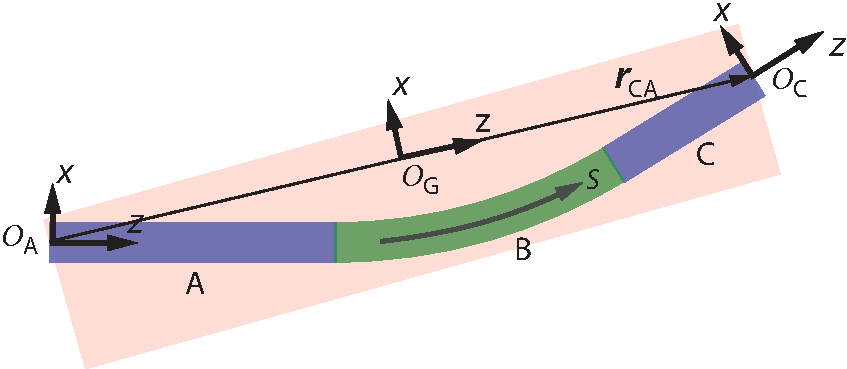
\includegraphics{girder.pdf}
  \caption[Girder example.] {
Girder supporting three elements labeled \vn{A}, \vn{B}, and \vn{C}.
$\calO_A$ is the reference frame at the upstream end of element \vn{A}
(\sref{s:ref.construct}), $\calO_C$ is the reference frame at the
downstream end of element \vn{C}, and $\calO_G$ is the default
\vn{origin} reference frame of the girder. $r_{CA}$ is the vector from
$\calO_A$ to $\calO_C$. The length \vn{l} of the girder is the
difference in $s$ between points $\calO_C$ and $\calO_A$.
  }
  \label{f:girder}
\end{figure}

A \vn{girder} is a support structure that orients the elements that
are attached to it in space. A girder can be used to simulate any
rigid support structure and there are no restrictions on how the lattice
elements that are supported are oriented with respect to one another.
Thus, for example, optical tables can be simulated.

General \vn{girder} attributes are:
\begin{center}
\tt
\begin{tabular}{llll} \toprule
  {\sl Attribute Class}      & Section           & {\sl Attribute Class}      & Section         \\ \midrule
  Custom Attributes          & \ref{s:cust.att}  & Length                     & \ref{s:l}       \\
  Description strings        & \ref{s:alias}     & Offsets, pitches \& tilt   & \ref{s:offset}  \\ 
  Is_on                      & \ref{s:is.on}     &                            &                 \\
  \bottomrule
\end{tabular}
\end{center}
\toffset
See \sref{s:list.girder} for a full list of element attributes along with a their units.

Attributes specific to a \vn{girder} are:
\index{origin_ele}\index{origin_ele_ref_pt}
\index{x_origin}\index{y_origin}
\index{z_origin}\index{theta_origin}
\index{phi_origin}\index{psi_origin}
Attributes specific to \vn{girder} elements are:
\begin{example}
  girder = \{<List>\}   ! List of elements on the Girder
  origin_ele        = <Name>     ! Reference element.
  origin_ele_ref_pt = <location> ! Reference pt on reference ele.
  dx_origin         = <Real>     ! x-position offset
  dy_origin         = <Real>     ! y-position offset
  dz_origin         = <Real>     ! z-position offset
  dtheta_origin     = <Real>     ! orientation angle offset.
  dphi_origin       = <Real>     ! orientation angle offset.
  dpsi_origin       = <Real>     ! orientation angle offset.
  l                 ! Girder "Length" (\ref{s:l}). Dependent attribute (\sref{s:depend}).
\end{example}

A simple example of a girder is shown in \fig{f:girder}. Here a girder supports three
elements labeled \vn{A}, \vn{B}, and \vn{C} where \vn{B} is a bend so the geometry is
nonlinear. Such a girder may specified in the lattice file like:
\begin{example}
  g1: girder = \{A, B, C\}
\end{example}

The \vn{girder} statement can take one of two forms:
\begin{example}
  <element_name>: GIRDER = \{<ele1>, <ele2>, ..., <eleN>\}, ... 
\end{example}
or
\begin{example}
  <element_name>: GIRDER = \{<ele_start>:<ele_end>\}, ... 
\end{example}

With the first form, a \vn{girder} element will be created for each section of the lattice where
there is a ``consecutive'' sequence of ``slave'' elements \vn{<ele1>} through \vn{<eleN>}.  This
section of the lattice from \vn{<ele1>} through \vn{<eleN>} is called the ``girder support region''.
``Consecutive'' here means there are no other elements in the girder support region except for
possibly \vn{drift} and/or \vn{marker} elements. \vn{Drift} elements cannot be controlled by a
girder\footnote{This policy was created to avoid the problem where the superposition of marker
elements on top of drifts would prevent girder formation.} but may appear in the girder slave
list. If a \vn{drift} does appear in the slave list, \vn{drift} elements will not be ignored when
determining if elements are consecutive. Note: If a drift-like element is desired to be supported by
a \vn{girder}, use a \vn{pipe} element instead. \vn{Marker} elements present in a girder support
region, but not mentioned in the girder slave list, are simply ignored.

The second form of a \vn{girder} statement specifies the first and last elements in the sequence of
elements to be supported. Everything in between except \vn{drift} elements will be supported by the
\vn{girder}.

Wild card characters (\sref{s:lat.attribs}) can be used in any element name in the girder slave
list. Additionally, beam line names (\sref{s:lines.wo.arg}) can be used. In this case, any
\vn{drift} elements within a beam line will be ignored.

A lattice element may have at most one \vn{girder} supporting it. However, a \vn{girder} can be
supported by another \vn{girder} which in turn can be supported by a third \vn{girder}, etc. Girders
that support other girders must be defined in the lattice file after the supported girders are
defined. Example:
\begin{example}
  g1: girder = \{A, B, C\}
  g2: girder = \{g1\}      ! g2 must come after g1!
\end{example}

A \vn{girder} may not directly support \vn{multipass_slave} (\sref{s:multipass}) or \vn{super_slave}
(\sref{s:super}) elements. Rather, a \vn{girder} may support the corresponding lord elements.

The reference frame from which the girder's offset, pitch, and tilt attributes (\sref{s:offset}) are
measured is constructed as follows: A reference frame, called the ``\vn{origin}'' reference frame
may be defined using the attributes \vn{origin_ele} and \vn{origin_ele_ref_pt} which constructs the
girder's \vn{origin} frame to be coincident with the reference frame of another element. Example:
\begin{example}
  g2: girder = \{...\}, origin_ele = Q, origin_ele_ref_pt = entrance_end
\end{example}
In this example, girder \vn{g2} has an \vn{origin} reference frame coincident with the entrance end
frame of an element named \vn{Q}. Valid values for \vn{origin_ele_ref_pt} are
\begin{example}
  entrance_end
  center        ! Default
  exit_end
\end{example}
For \vn{crystal}, \vn{mirror}, and \vn{multilayer_mirror} elements, setting \vn{origin_ele_ref_pt}
to \vn{center} results in the reference frame being the frame of the surface (cf.~\fig{f:surface}).

To specify that the global coordinates (\sref{s:global}) are to be used for a girder set
\vn{origin_ele} to \vn{global_coordinates}. Typically this is the same as using the \vn{beginning}
element (\sref{s:begin.ele}) as the \vn{origin_ele} except when the \vn{beginning} element is offset
or reoriented (\sref{s:beginning}).

If \vn{origin_ele} is not given, the default \vn{origin} frame is used. The default \vn{origin}
frame is constructed as follows: Let $\calO_A$ be the reference frame of the upstream end of the
first element in the list of supported elements. In this example it is the upstream end of element
\vn{A} as shown in the figure. Let $\calO_C$ be the downstream end of the last element in the list
of supported elements. In this example this is the downstream end of element \vn{C}. The origin of
the \vn{girder}'s reference frame, marked $\calO_G$ in the figure, will be half way along the vector
$r_{CA}$ from the origin of $\calO_A$ to the origin of $\calO_B$.  The orientation of $\calO_G$ is
constructed by rotating the $\calO_A$ coordinate system along an axis in $\calO_A$'s $x$-$y$ plane
such that $\calO_A$'s $z$ axis ends up parallel with $r_{CA}$. In the example above, the rotation
axis will be along $\calO_A$'s $y$-axis.

Once the \vn{origin} reference frame is established, the reference frame of the girder can be offset
from the \vn{origin} frame using the parameters
\begin{example}
  dx_origin    dtheta_origin
  dy_origin    dphi_origin
  dz_origin    dpsi_origin
\end{example} 
The orientation of the \vn{girder}'s reference frame from the \vn{origin}
frame is given in \sref{s:patch.coords}. Example:
\begin{example}
  g3: girder = \{ ... \}, dx_origin = 0.03
\end{example}
This offsets girder \vn{g3}'s reference frame 3~cm horizontally from
the default \vn{origin} frame. If no offsets are given, the
\vn{origin} frame is the same as the girder's reference frame.

The length \vn{l} of a girder, which is not used in any calculations,
is a dependent attribute computed by \bmad and set equal to the $s$
path length between points $\calO_C$ and $\calO_A$.

\index{x_offset}\index{y_offset}\index{x_pitch}\index{y_pitch}\index{tilt}
The physical orientation of the girder with respect to it's reference
frame is, like other elements, determined by the offset, pitch and
tilt orientation attributes as outlined in \sref{s:offset} and
\sref{s:patch.coords}.  When a girder is shifted in space, the elements
it supports are also shifted.  In this case, the orientation
attributes (\vn{x_offset}, \vn{y_pitch}, etc.) give the orientation of
the element with respect to the \vn{girder}. The orientation with
respect to the local reference coordinates is given by
\vn{x_offset_tot}, which are computed from the orientation attributes
of the element and the \vn{girder}. An example will make this clear:
\begin{example}
  q1: quad, l = 2
  q2: quad, l = 4, x_offset = 0.02, x_pitch = 0.01
  d: drift, l = 8
  g4: girder = \{q1, q2\}, x_pitch = 0.002, x_offset = 0.03
  this_line: line = (q1, d, q2)
  use, this_line
\end{example}
\index{overlay}
In this example, \vn{g4} supports quadrupoles \vn{q1} and \vn{q2}.
Since the supported elements are colinear, the computation is greatly
simplified. The reference frame of \vn{g4}, which is the default
\vn{origin} frame, is at $s = 7$~meters which is half way between the
start of \vn{q1} at at $s = 0$~meters and the end of \vn{q2}) which is
at $s = 14$. The reference frames of \vn{q1} and \vn{q2} are at their
centers so the $s$ positions of the reference frames is
\begin{example}
  Element        S_ref   dS_from_g4
  q1             1.0     -6.0
  g4             7.0      0.0
  q2            12.0      5.0
\end{example}
Using a small angle approximation to simplify the calculation, the \vn{x_pitch} of \vn{g4} produces
an offset at the center of \vn{q2} of $0.01 = 0.002 * 5$. This, added to the offsets of \vn{g4} and
\vn{q2}, give the total \vn{x_offset}, denoted \vn{x_offset_tot} of \vn{q2} is $0.06 = 0.01 + 0.03 +
0.02$. The total \vn{x_pitch}, denoted \vn{x_pitch_tot}, of \vn{q2} is $0.022 = 0.02 + 0.001$.

A \vn{girder} that has its \vn{is_on} attribute set to False is considered to be unsifted with
respect to it's reference frame.

\newpage

%-----------------------------------------------------------------------------
\section{GKicker}
\label{s:gkicker}
\index{gkicker|hyperbf}

A \vn{gkicker} element is a ``general'' zero length kicker element that can displace
a particle in all six phase space dimensions.

General \vn{group} attributes are:
\begin{center}
\tt
\begin{tabular}{llll} \toprule
  {\sl Attribute Class}      & Section           & {\sl Attribute Class}      & Section         \\ \midrule
  Custom Attributes          & \ref{s:cust.att}  & Description strings        & \ref{s:alias}   \\ 
  \bottomrule
\end{tabular}
\end{center}
\toffset
See \sref{s:list.group} for a full list of element attributes along with a their units.

Attributes specific to a \vn{gkicker} are:
\index{x_kick}\index{px_kick}\index{y_kick}\index{py_kick}\index{z_kick}\index{pz_kick}
\begin{example}
  x_kick        = <Real>  ! X-position kick
  px_kick       = <Real>  ! X-momentum kick
  y_kick        = <Real>  ! Y-position kick
  py_kick       = <Real>  ! Y-momentum kick
  z_kick        = <Real>  ! Z-position kick
  pz_kick       = <Real>  ! Momentum kick
\end{example}

Example:
\begin{example}
  gk: gkicker, x_kick = 0.003, pz_kick = 0.12
\end{example}

\newpage

%-----------------------------------------------------------------------------
\section{Group}
\label{s:group}
\index{group|hyperbf}

\vn{Group} elements are a type of \vn{control} element (\sref{s:lord.slave}) used to make variations
in the attributes of other elements (called ``slave'' attributes) during execution of a program. For
example, to simulate the action of a control room knob that changes the beam tune in a storage ring,
a \vn{group} element can be used to vary the strength of selected quads in a specified manner. Also
see \vn{overlay} (\sref{s:overlay}) The difference between \vn{group} and \vn{overlay} elements is
that \vn{overlay} elements set the values of the attributes directly while \vn{group} elements make
delta changes to attribute values.

General \vn{group} attributes are:
\begin{center}
\tt
\begin{tabular}{llll} \toprule
  {\sl Attribute Class}      & Section           & {\sl Attribute Class}      & Section         \\ \midrule
  Custom Attributes          & \ref{s:cust.att}  & Description strings        & \ref{s:alias}   \\ 
  \bottomrule
\end{tabular}
\end{center}
\toffset
See \sref{s:list.group} for a full list of element attributes along with a their units.

There are two types of \vn{group} elements: \vn{Expression} based and \vn{knot} based.
The general syntax for a \vn{expression} based \vn{group} element is
\begin{example}
  name: GROUP = \{ele1[attrib1]:exp1, ele2[attrib2]:exp2, ...\}, 
              VAR = \{var1, var2, ...\}, var1 = init_val1, old_var1 = init_val_old1, ...
\end{example}
where \vn{ele1}[\vn{attrib1}], \vn{ele2}[\vn{attrib2}], etc. specify the slave attributes and
\vn{exp1}, \vn{exp2}, etc. are the arithmetical expressions, that are functions of \vn{var1},
\vn{var2}, etc., and are used to determine a value for the slave attributes.

The general syntax for a \vn{knot} based  \vn{group} element is
\begin{example}
  name: GROUP = \{ele1[attrib1]:\{y_knot_points1\}, ele2[attrib2]:\{y_knot_points2\}, ...\}, 
              VAR = \{var1\}, X_KNOT = \{x_knot_points\}, INTERPOLATION = \{type\}, 
              var1 = init_val1, old_var1 = init_val_old1, ...
\end{example}
When using knot points, the \vn{group} may only have one variable parameter.

\textbf{See Section~\sref{s:go.syntax} for a detailed description of this syntax.}

Example of a \vn{expression} based \vn{group} element:
\begin{example}
  gr1: group = \{q[k1]:a+b^2\}, var = \{a, b\}, a = 1, old_a = 2
  gr1[old_b] = 2
\end{example}
There are two numbers associated with each variable in a group: One number is the value of the
variable (also called the ``present'' value) and the other number is the ``old'' value. To refer to
these old values prepend the string ``old_'' to the variable name. Thus, in the above example, the
old variable values have names \vn{old_a} and \vn{old_b} and these old values can be set in the same
manner as the present values.

Example of a \vn{knot} based \vn{group} element:
\begin{example}
  gr2: group = \{beginning[E_tot]]:\{4e6,...\}\}, 
      var = \{time\}, x_knot = \{...\}, interpolate = cubic
\end{example}
Here the function used to translate from the \vn{group}'s variables to the slave attribute values is
a cubic spline interpolation based upon the knot points specified (\sref{s:go.syntax}).

A \vn{group} element is like an \vn{overlay} element in that a \vn{group} element controls the
attribute values of other ``slave'' elements. The difference is that the value of a slave attribute
that is controlled by (one or more) \vn{overlay} elements is uniquely determined by the controlling
\vn{overlay} elements. A \vn{group} element, on the other hand, is used to make changes in
value. An example will make this clear:
\begin{example}
  gr: group = \{q1[k1]:0.1*a^2\}, var = \{a\}, a = 2, old_a = 1
  q, quad, k1 = 0.5
\end{example}
When a program reads the lattice file, initially the value of \vn{q[k1]} will be 0.5 as set
in the definition of \vn{q}. Later, during lattice expansion (\sref{s:expand}), the group elements
are added to the lattice. When the group element \vn{gr} is added, the fact that \vn{old_a} and
\vn{a} are different causes the value of \vn{q[k1]} to be modified. The delta value is
\begin{example}
  delta = 0.1*a^2 - 0.1*old_a^2
        = 0.3
\end{example}
And this is added to the existing value of 0.5 so that the value of \vn{q[k1]} becomes 0.8.  After
the value of \vn{q[k1]} has been updated, the value of \vn{old_a} is automatically update to be the
present value of \vn{a} so that the value of \vn{q[k1]} will not be further modified.

In general, deltas used to modify slave attributes are computed as the difference between the
arithmetic expression evaluated with the present variable values and the arithmetic expression
evaluated with the old variable values.

Notice that in a lattice file the value of a slave attribute after the lattice is read in is
independent of whether the group is defined before or after elements whose attributes are controlled
by the group. This is true since the effect of a \vn{group} element happens when the lattice is
expanded, not when parser reads the \vn{group} definition. On the other hand, after the lattice has
been read in, if a program varies both a group variable and a slave attribute, the value of the
slave attribute will be dependent upon the order of which is modified first. For example, consider a
lattice containing:
\begin{example}
  gr: group = \{q[k1]:a^2\}, var = \{a\} 
  q, quad
\end{example}
Now if a program first sets \vn{gr[a]} to 0.3 and then sets \vn{q[k1]} to 0.5, the result is that
\vn{q[k1]} will have a value of 0.5. That is, the value of \vn{q[k1]} will be independent of
\vn{gr[a]}. If the setting is reversed so that \vn{q[k1]} is set first, the value of \vn{q[k1]} will
be 0.59. Since the result is order dependent, trying to ``simultaneously'' vary the attributes of
both group variables and slave attributes can lead to unpredictable results. For example, consider
lattice ``optimization'' where a program varies a set of lattice parameters to achieve certain goals
(for example, minimum beta at some point in the lattice, etc.). If the list of parameters to be
varied contains both group variables and slave attributes, the actual changes to slave attributes
may be different from what the user expects when the program varies its list of parameters.

\index{overlay}\index{girder}
Different \vn{group} elements may control the same slave attribute and a \vn{group} element may
control other \vn{group}, \vn{overlay} or \vn{girder} element attributes. However, It does not make
sense, and it is not permitted, for a \vn{group} element to control the same attribute as an
\vn{overlay} element or for a \vn{group} element to control a \vn{dependent} attribute
(\sref{s:depend}). To setup a group element to control the same slave attribute as an \vn{overlay},
define an intermediate \vn{overlay}. For example:
\begin{example}
  ov: overlay = \{q{k1}\, q2[k1], ...\}, var = \{a\}
  q, quad                                          
  gr: group = \{ov_q[k1]:a^2\}, var = \{a\}  ! New
  ov_q: overlay = \{q\}, var = \{k1\}        ! New
\end{example}
In this example, the overlay \vn{ov} controls the attribute \vn{q[k1]} so it is not permitted for
\vn{q[k1]} to be a slave of a group element.  To have group control of \vn{q[k1]}, two elements are
introduced: the group \vn{gr} is setup controlling \vn{ov_q[k1]} and overlay \vn{ov_q} is an overlay
that controls \vn{q[k1]}. Notice that trying to control \vn{ov} directly by a group element will not
work since \vn{ov} controls multiple elements.

\index{accordion_edge}\index{start_edge}
\index{end_edge}\index{symmetric_edge}
\index{z_offset}
A \vn{group} can be used to control an elements position and length
using one of the following attributes:
\begin{example}
  accordion_edge  ! Element grows or shrinks symmetrically
  start_edge      ! Varies element's upstream edge s-position
  end_edge        ! Varies element's downstream edge s-position
  s_position      ! Varies element's overall s-position. Constant length.
\end{example}
With \vn{accordion_edge}, \vn{start_edge}, \vn{end_edge}, and \vn{symmetric_edge} the longitudinal
position of an elements edges are varied. This is done by appropriate control of the element's
length and the lengths of the elements to either side. In all cases the total length of the lattice
is kept invariant.

As an example, consider \vn{accordion_edge} which varies the edges of an element so that the center
of the element is fixed but the length varies:
\begin{example}
  gr: group = \{Z[accordion_edge]:1\}, var = \{offset\}
\end{example}
A change of, say, 0.1 \vn{gr}'s \vn{offset} variable moves both edges of element \vn{Z} by 0.1
meters so that the length of \vn{Z} changes by 0.2 meters but the center of \vn{Z} is constant. To
keep the total lattice length invariant, the lengths of the elements to either side are decreased by
0.1 meters to keep the total lattice length constant.
\begin{example}
  q10: quad, l = ...
  q11: quad, l = ...
  d1: drift, l = ...
  d2: drift, l = ...
  this_line: line = (... d1, q10, d2, q11, ...)
  gr2: group = \{q10[start_edge]:1\}, var = \{a\}, a = 0.1
\end{example}
The effect of  \vn{gr2[a]} will be to lengthen the length of
\vn{q10} and shorten the length of \vn{d1}.

A lattice file may contain lines and lattice elements that are not part of the actual finished
lattice when the lattice is constructed. \vn{Group} elements where {\em none} of its slave elements
are part of the finished lattice are ignored and are also not part of the finished lattice.  When a
\vn{group} element has some slave elements that are part of the finished lattice and some slave
elements that are not, the \vn{group} element as implemented in the finished lattice will only
control slave elements that actually exist in the finished. In any case, a slave element that a
\vn{group} element references must be defined (but not necessarily be used in the finished lattice)
in the lattice file. This rule is enforced in order to catch spelling mistakes.

If the arithmetical expression used for an \vn{group} contains an element attribute, care must be
taken if that element attribute is changed. This is discussed in \sref{s:arith} and
\sref{s:go.syntax}.

\newpage

%-----------------------------------------------------------------
\section{Hybrid}
\label{s:hybrid}
\index{hybrid|hyperbf}

A \vn{hybrid} element is an element that is formed by a program by concatenating other element
together. \vn{Hybrid} elements are used to reduce the number of elements in a lattice to speed up a
simulation. In terms of tracking a \vn{hybrid} element is essentially the same as a \vn{taylor}
element.

\newpage

%-----------------------------------------------------------------
\section{Instrument, Monitor, and Pipe}
\label{s:monitor}
\index{instrument|hyperbf}
\index{monitor|hyperbf}
\index{pipe|hyperbf}

Essentially \bmad treats \vn{instrument}, \vn{monitor}, and \vn{pipe} elements like a
\vn{drift}. There is a difference, however, when superimposing elements (\sref{s:super}). For
example, a \vn{quadrupole} superimposed on top of a \vn{drift} results in a free \vn{quadrupole}
element in the tracking part of the lattice and no lord elements are created. On the other hand, a
\vn{quadrupole} superimposed on top of a \vn{monitor} results in a \vn{quadrupole} element in the
tracking part of the lattice and this \vn{quadrupole} element will have two lords: A \vn{quadrupole}
superposition lord and a \vn{monitor} superposition lord. The exception is if a \vn{instrument},
\vn{monitor}, and \vn{pipe} is superimposed with an element with non-constant reference energy like
a \vn{lcavity}. In this case no \vn{instrument}, \vn{monitor}, or \vn{pipe} \vn{super_lord} element
is made.

General \vn{instrument}, \vn{monitor}, and \vn{pipe} attributes are:
\begin{center}
\tt
\begin{tabular}{llll} \toprule
  {\sl Attribute Class}      & Section             & {\sl Attribute Class}      & Section         \\ \midrule
  Aperture limits            & \ref{s:limit}       & Is_on                      & \ref{s:is.on}   \\
  Chamber wall               & \ref{s:wall}        & Length                     & \ref{s:l}       \\
  Custom Attributes          & \ref{s:cust.att}    & Offsets, pitches \& tilt   & \ref{s:offset}  \\ 
  Description strings        & \ref{s:alias}       & Reference energy           & \ref{s:energy}  \\
  Hkick \& Vkick             & \ref{s:kick}        & Superposition              & \ref{s:super}   \\
  Instrumental variables     & \ref{s:meas.attrib} & Symplectify                & \ref{s:symp}    \\
  Integration settings       & \ref{s:integ}       & Tracking \& transfer map   & \ref{c:methods} \\
  \bottomrule
\end{tabular}
\end{center}
\toffset
See \sref{s:list.instrument} for a full list of element attributes along with a their units.

\index{x_offset}
\index{y_offset}
\index{x_pitch}
\index{y_pitch}
\index{tilt}
The \vn{offset}, \vn{pitch}, and \vn{tilt} attributes are not
used by any \bmad routines. If these attributes are used by a program
they are typically used to simulate such things as measurement
offsets. The \vn{is_on} attribute is also not used by \bmad
proper. Example:
\begin{example}
  d21: instrum, l = 4.5
\end{example}

\newpage

%-----------------------------------------------------------------
\section{Kickers: Hkicker and Vkicker}
\label{s:hvkicker}
\index{hkicker|hyperbf}
\index{vkicker|hyperbf}

An \vn{hkicker} gives a beam a horizontal kick and a \vn{vkicker} gives a 
beam a vertical kick. Also see the \vn{kicker} (\sref{s:kicker}) element.

General \vn{hkicker} \vn{vkicker} attributes are:
\begin{center}
\tt
\begin{tabular}{llll} \toprule
  {\sl Attribute Class}      & Section           & {\sl Attribute Class}      & Section         \\ \midrule
  Aperture limits            & \ref{s:limit}     & Is_on                      & \ref{s:is.on}   \\
  Chamber wall               & \ref{s:wall}      & Length                     & \ref{s:l}       \\
  Custom Attributes          & \ref{s:cust.att}  & Mag \& Elec multipoles     & \ref{s:multip}  \\
  Description strings        & \ref{s:alias}     & Offsets, pitches \& tilt   & \ref{s:offset}  \\
  Field Maps                 & \ref{s:fieldmap}  & Reference energy           & \ref{s:energy}  \\ 
  Fringe Fields              & \ref{s:fringe}    & Superposition              & \ref{s:super}   \\
  Hkick \& Vkick             & \ref{s:kick}      & Symplectify                & \ref{s:symp}    \\
  Integration settings       & \ref{s:integ}     & Tracking \& transfer map   & \ref{c:methods} \\
  \bottomrule
\end{tabular}
\end{center}
\toffset
See \sref{s:list.hvkicker} for a full list of element attributes along with a their units.

\index{kick}
\index{hkick}
\index{vkick}
Note that \vn{hkicker} and \vn{vkicker} elements use the
\vn{kick} attribute while a \vn{kicker} uses the \vn{hkick} and \vn{vkick} 
attributes. Example:
\begin{example}
  h_kick: hkicker, l = 4.5, kick = 0.003
\end{example}

\newpage

%-----------------------------------------------------------------
\section{Kicker}
\label{s:kicker}
\index{kicker|hyperbf}

\index{hkick}\index{vkick}
\index{h_displace}\index{v_displace}
A \vn{kicker} can deflect a beam in both planes. Note that a \vn{kicker} uses the \vn{hkick} and
\vn{vkick} attributes while \vn{hkicker} and \vn{vkicker} elements use the \vn{kick} attribute.  In
addition, a \vn{kicker} can apply a displacement to a particle using the \vn{h_displace} and
\vn{v_displace} attributes.

General \vn{kicker} attributes are:
\begin{center}
\tt
\begin{tabular}{llll} \toprule
  {\sl Attribute Class}      & Section           & {\sl Attribute Class}      & Section          \\ \midrule
  Mag \& Elec multipoles     & \ref{s:multip}    & Length                     & \ref{s:l}        \\
  Aperture limits            & \ref{s:limit}     & Offsets, pitches \& tilt   & \ref{s:offset}   \\
  Chamber wall               & \ref{s:wall}      & Overlapping Fields         & \ref{s:overlap}  \\
  Custom Attributes          & \ref{s:cust.att}  & Reference energy           & \ref{s:energy}   \\ 
  Description strings        & \ref{s:alias}     & Superposition              & \ref{s:super}    \\
  Fringe Fields              & \ref{s:fringe}    & Symplectify                & \ref{s:symp}     \\
  Hkick \& Vkick             & \ref{s:kick}      & Field Maps                 & \ref{s:fieldmap} \\
  Integration settings       & \ref{s:integ}     & Tracking \& transfer map   & \ref{c:methods}  \\ 
  Is_on                      & \ref{s:is.on}     &                            &                  \\
  \bottomrule
\end{tabular}
\end{center}
\toffset
See \sref{s:list.kicker} for a full list of element attributes along with a their units.

Example:
\begin{example}
  a_kick: kicker, l = 4.5, hkick = 0.003
\end{example}

\newpage

%-----------------------------------------------------------------
\section{Lcavity}
\label{s:lcav}
\index{lcavity|hyperbf}

An \vn{lcavity} is a LINAC accelerating cavity.  The main difference between an \vn{rfcavity} and an
\vn{lcavity} is that, unlike an \vn{rfcavity}, the reference energy (\sref{s:ref.energy}) through
an \vn{lcavity} is not constant.

General \vn{lcavity} attributes are:
\begin{center}
\tt
\begin{tabular}{llll} \toprule
  {\sl Attribute Class}      & Section           & {\sl Attribute Class}      & Section            \\ \midrule
  Aperture limits            & \ref{s:limit}     & Offsets, pitches \& tilt   & \ref{s:offset}     \\
  Chamber wall               & \ref{s:wall}      & Overlapping Fields         & \ref{s:overlap}    \\
  Custom Attributes          & \ref{s:cust.att}  & Reference energy           & \ref{s:energy}     \\ 
  Description strings        & \ref{s:alias}     & RF Couplers                & \ref{s:rf.coupler} \\
  Field autoscaling          & \ref{s:autoscale} & Superposition              & \ref{s:super}      \\
  Fringe Fields              & \ref{s:fringe}    & Symplectify                & \ref{s:symp}       \\
  Hkick \& Vkick             & \ref{s:kick}      & Field Maps                 & \ref{s:fieldmap}   \\
  Integration settings       & \ref{s:integ}     & Tracking \& transfer map   & \ref{c:methods}    \\
  Is_on                      & \ref{s:is.on}     & Wakes                      & \ref{s:wakes}      \\
  Length                     & \ref{s:l}         &                            &                    \\
  \bottomrule
\end{tabular}
\end{center}
\toffset
See \sref{s:list.lcavity} for a full list of element attributes along with a their units.

The attributes specific to an \vn{lcavity} are 
\index{gradient}\index{phi0}\index{n_cell}
\index{phi0_multipass}\index{e_loss}
\index{rf_frequency}\index{voltage}\index{cavity_type}
\begin{example}
  cavity_type     = <Switch>  ! Type of cavity.
  gradient        = <Real>    ! Accelerating gradient (V/m).
  gradient_err    = <Real>    ! Accelerating gradient error (V/m).
  gradient_tot                ! Net gradient = gradient + gradient_err. Dependent param (\sref{s:depend}).
  phi0            = <Real>    ! Phase (rad/2\(\pi\)) of the reference particle with 
                              !   respect to the RF. phi0 = 0 is on crest.
  phi0_autoscale              ! Set by Bmad when autoscaling is turned on \sref{s:autoscale}.
  phi0_multipass  = <Real>    ! Phase (rad/2\(\pi\)) with respect to a multipass lord (\sref{s:multipass}).
  phi0_err        = <Real>    ! Phase error (rad/2\(\pi\))
  e_loss          = <Real>    ! Loss parameter for short range wakefields (V/Coul).
  rf_frequency    = <Real>    ! RF frequency (Hz).
  field_autoscale             ! Set by Bmad when autoscaling is turned on \sref{s:autoscale}.
  voltage                     ! Cavity voltage. Dependent attribute (\sref{s:depend}).
  voltage_err                 ! Error voltage
  voltage_tot                 ! Net voltage = voltage + voltage_err. Dependent param (\sref{s:depend}).
  l_active        = <Real>    ! Active region length. Dependent attribute (\sref{s:depend}).
  n_cell          = <Int>     ! Number of cavity cells. Default is 1.
  longitudinal_mode = <Int>   ! Longitudinal mode. Default is 1. May be 0 or 1.
\end{example}

The \vn{voltage} and \vn{voltage_err} attributes can be used in place of \vn{gradient} and \vn{gradient_err}.
The relationship between gradient and voltage is
\begin{example}
  voltage     = L * gradient
  voltage_err = L * gradient_err
\end{example}

The energy kick felt by a particle, assuming no phase slippage, is 
\begin{example}
  dE = \(r_q\) * gradient_tot * L * cos(\(2\,\pi\) * (\(\phi_t\) + \(\phi_\REF\)))
\end{example}
where $r_q$ is the charge of the particle relative to the charge of the reference particle.
\index{multipass}
where the total gradient is
\begin{example}
  gradient_tot = (gradient + gradient_err) * field_autoscale
\end{example}
$\phi_t$ is the part of the phase due to when the particle arrives at the cavity and depends upon
whether \vn{absolute time tracking} or \vn{relative time tracking} is being used as discussed in
\sref{s:rf.time}. The phase $\phi_\REF$ is
\begin{example}
  \(\phi_\REF\) = phi0 + phi0_multipass + phi0_err + phi0_autoscale
  \label{lcav.phi}
\end{example}

In the above equation $r_q$ is the relative charge between the reference particle (set by the
\vn{parameter[particle]} parameter in a lattice file) and the particle being tracked through the
cavity. For example, if the reference particle and and the tracked particle are the same, $r_q$ is
unity independent of the type of particle tracked.

\vn{phi0_multipass} is only to be used with multipass to shift the phase of the cavity from pass to
pass. See \sref{s:multipass}.

\vn{phi0_autoscale} and \vn{field_autoscale} are calculated by \bmad's auto-scale module. See
Section~\sref{s:autoscale} for more details. Autoscaling can be toggled on/off by using the
\vn{autoscale_phase} and \vn{autoscale_amplitude} toggles.

The energy change of the reference particle is just the energy change for a 
particle with $z = 0$ and no phase or gradient errors. Thus
\begin{example}
  dE(reference) = gradient * L * cos(\(2\,\pi\) * \(\phi_\REF\))
\end{example}

The energy kick for a \bmad \vn{lcavity} is consistent with MAD. 
Note: The MAD8 documentation for an \vn{lcavity} has a wrong
sign. Essentially the MAD8 documentation gives
\begin{example}
  dE = gradient * L * cos(\(2\,\pi\) * (\(\phi_\REF\) - phi(z))) ! WRONG
\end{example}
This is incorrect. 

When short-range wakefields are being simulated, with \vn{bmad_com%sr_wakes_on = True}
(\sref{s:bmad.ptc.com}), the \vn{e_loss} attribute can be used to modify the gradient in order to
maintain a constant average energy gain. That is, \vn{e_loss} can be used to simulate the effect of
a feedback circuit that attempts to maintain the average energy of the bunch after the element
constant.  The energy kick is then
\begin{example}
  dE(with wake) = dE + e_loss * n_part * e_charge 
\end{example}
\vn{n_part} is set using the \vn{parameter} statement (\sref{s:param}) and represents the number of
particles in a bunch. \vn{e_charge} is the magnitude of the charge on an electron
(Table~\ref{t:constants}). Notice that the \vn{e_loss} term is independent of the sign of the charge
of the particle.

The \vn{cavity_type} is the type of cavity being simulated. Possible
settings are:
\begin{example}
  ptc_standard
  standing_wave    ! Default
  traveling_wave
\end{example}
The \vn{cavity_type} switch is ignored if a field map is used.  With the \vn{standing_wave} setting,
the transverse trajectory through an \vn{lcavity} is modeled using equations developed by Rosenzweig
and Serafini\cite{b:rosenzweig} modified to give the correct phase-space area at non
ultra-relativistic energies.  See Section \sref{s:lcavity.std} for more details.  Note: The transfer
matrix for an \vn{lcavity} with finite \vn{gradient} is never symplectic. See
\sref{s:phase.space}. In addition, couplers (\sref{s:rf.coupler}) and HOM wakes (\sref{s:wakes}) can
be modeled.

When an element's \vn{tracking_method} is set to \vn{runge_kutta}, the fields used with
\vn{field_calc} set to \vn{bmad_standard} are described in Section~(\sref{s:rf.fields}). With
\vn{cavity_type} set to \vn{standing_wave}, the longitudinal mode is set by the
\vn{longitudinal_mode} parameter. The possible values are 0 or 1 and the default setting is 0.

If an element's \vn{cavity_type} parameter is set to \vn{standing_wave}, and if the \vn{field_calc}
parameter is set to \vn{bmad_standard}, and if an element's \vn{tracking_method} is set to
\vn{runge_kutta} (\sref{s:tkm}), the ``active region'' over which there is a finite field is
\vn{n_cell} half-wave pillbox resonators where each pillbox has length $\lambda/2$
(\sref{s:rf.fields}). The default setting for \vn{n_cell} is 1. The dependent parameter
\vn{l_active} is set to the length of the active region. The active region should have a length less
than the length of the element. If the length of the element is not equal to the active region, the
active region is centered in the element and the regions to either side are treated as field free.

Note: When an element's \vn{tracking_method} is set to \vn{bmad_standard}, settings for the
parameters \vn{n_cell}, and \vn{longitudinal_mode} are ignored.

Example:
\begin{example}
  lwf: lcavity, l = 2.3, rf_frequency = 500e6, voltage = 20e6,
         tracking_method = runge_kutta, n_cell = 3, longitudinal_mode = 1
\end{example}

{\em Note: The default \vn{bmad_standard} tracking for \vn{lcavity} elements when the velocity
$\beta$ is significantly different from 1 can only be considered as a rough approximation. Indeed,
the only accurate way to simulate a cavity in this situation is by integrating through the actual
field [Cf.~Runge Kutta tracking (\sref{s:tkm})]}

\newpage

%-----------------------------------------------------------------
\section{Lens}
\label{s:lens}
\index{lens|hyperbf}

A \vn{lens} is an element for concentrating or dispersing light rays.

This element is under development...

\newpage

%-----------------------------------------------------------------
\section{Marker}
\label{s:mark}
\index{marker|hyperbf}

A \vn{marker} is a zero length element meant to mark a position. 

General \vn{marker} attributes are:
\begin{center} 
\tt
\begin{tabular}{llll} \toprule
  {\sl Attribute Class}      & Section             & {\sl Attribute Class}        & Section         \\ \midrule
  Aperture limits            & \ref{s:limit}       & Is_on                        & \ref{s:is.on}   \\ 
  Chamber wall               & \ref{s:wall}        & Offsets \& tilt              & \ref{s:offset}  \\
  Custom Attributes          & \ref{s:cust.att}    & Reference energy             & \ref{s:energy}  \\
  Description strings        & \ref{s:alias}       & Superposition                & \ref{s:super}   \\
  Instrumental variables     & \ref{s:meas.attrib} & Tracking \& transfer map     & \ref{c:methods} \\ 
  \bottomrule
\end{tabular}
\end{center}
\toffset
See \sref{s:list.marker} for a full list of element attributes along with a their units.

\index{x_offset}\index{y_offset}
\index{tilt}\index{is_on}
The \vn{x_offset}, \vn{y_offset} and \vn{tilt} attributes are not used
by any \bmad routines. Typically, if these attributes are used by a
program, they are used to simulate things like BPM offsets. The
\vn{is_on} attribute is also not used by \bmad proper. 

Example:
\begin{example}
  mm: mark, type = "BPM"
\end{example}

\newpage

%-----------------------------------------------------------------
\section{Mask}
\label{s:mask}
\index{mask|hyperbf}

A \vn{mask} element defines an aperture where the mask area can
essentially have an arbitrary shape. 

For X-ray tracking, a \vn{mask} element is similar to a
\vn{diffraction_plate} (\sref{s:diff.plate}) element except that with
a \vn{diffraction_plate} element, coherent effects are taken into
account while, with a \vn{mask} element, coherent effects are ignored.
Also a \vn{mask} element can be used with charged particles while a
\vn{diffraction_plate} cannot.

General \vn{mask} element attributes are:
\begin{center}
\tt 
\begin{tabular}{llll} \toprule
  {\sl Attribute Class}      & Section           & {\sl Attribute Class}      & Section         \\ \midrule
  Aperture limits            & \ref{s:limit}     & Offsets, pitches \& tilt   & \ref{s:offset}  \\
  Custom Attributes          & \ref{s:cust.att}  & Reference energy           & \ref{s:energy}  \\
  Description strings        & \ref{s:alias}     & Superposition              & \ref{s:super}   \\
  Is_on                      & \ref{s:is.on}     & Tracking \& transfer map   & \ref{c:methods} \\
  \bottomrule
\end{tabular}
\end{center}
\toffset
See \sref{s:list.mask} for a full list of element attributes along with a their units.

Notice that, unlike a \vn{rcollimator} or a \vn{ecollimator}, a \vn{mask} element has zero length.

\index{mode}\index{field_scale_factor}
Attributes specific to a \vn{mask} element are:
\begin{example}
  mode               = <Type>   ! Reflection or transmission (photon tracking only).
  field_scale_factor = <Real>   ! Factor to scale the photon field.
  ref_wavelength                ! Reference wavelength (\sref{s:energy}). Dependent attrib (\sref{s:depend}).
  wall               = \{...\}    ! Defines mask geometry (\ref{s:wall}, \ref{s:masking.wall}).

\end{example}

Note: These attributes are only pertinent for photon tracking. Charged
particle tracking assumes transmission mode and does not use
\vn{field_scale_factor} and \vn{ref_wavelength} attributes.

The \vn{mode} switch, which is only used for photon tracking, sets
whether X-rays are transmitted through the \vn{mask} or
or reflected. Possible values for the \vn{mode} switch are:
\begin{example}
  reflection
  transmission        ! Default
\end{example}

The geometry of the mask, that is, where the openings (in transmission mode) or reflection regions
are, is defined using the ``wall'' attribute. See \sref{s:wall} and \ref{s:masking.wall} for more
details.

In transmission mode, a \vn{mask} is nominally orientated transversely to the beam. Like all other
elements, the \vn{mask} can be reoriented using the element's offsets, pitches and tilt attributes
(\sref{s:offset}).

\index{aperture_type}
The \vn{aperture_type} (\sref{s:limit}) parameter of a \vn{mask} will default to \vn{auto} which
will set the aperture limits to define a rectangular aperture that just cover the clear area of the
mask.

\index{field_scale_factor}
The \vn{field_scale_factor}, if set to a non-zero value (zero is the
default) will be used to scale the field of photons as they pass through
the \vn{mask} element:
\begin{example}
  field -> field * field_scale_factor
\end{example}
Scaling is useful since the electric field of photons traveling through a \vn{mask} are renormalized
(see \Eqs{eeo4p} and \eq{eek4p}). This can lead to large variation of the photon field and can, for
example, make visual interpretation of plots of field verses longitudinal position difficult to
interpret. \vn{field_scale_factor} can be used to keep the field more or less constant.

A \vn{mask} that is ``turned off'' (\vn{is_on} attribute set to False), does not mask at all and
transmits everything.

Example:
\begin{example}
scrapper: mask, mode = transmission, wall = \{
    section = \{type = clear, v(1) = \{0.9, 0.5\}\},
    section = \{type = opaque, r0 = (0, 0.4), v(1) = \{0.1, 0.1\}\}
  \}
\end{example}

\newpage

%-----------------------------------------------------------------
\section{Match}
\label{s:match}
\index{match|hyperbf}

A \vn{match} element is used to match the Twiss parameters between two
points. 

General \vn{match} attributes are:
\begin{center} 
\tt
\begin{tabular}{llll} \toprule
  {\sl Attribute Class}      & Section           & {\sl Attribute Class}      & Section         \\ \midrule
  Aperture limits            & \ref{s:limit}     & Length                     & \ref{s:l}       \\
  Custom Attributes          & \ref{s:cust.att}  & Reference energy           & \ref{s:energy}  \\ 
  Description strings        & \ref{s:alias}     & Superposition              & \ref{s:super}   \\ 
  Is_on                      & \ref{s:is.on}     &                            &                 \\
  \bottomrule
\end{tabular}
\end{center}
\toffset
See \sref{s:list.match} for a full list of element attributes along with a their units.

Attributes specific to a \vn{match} element are:
\begin{example}
  beta_a0, beta_b0   = <Real>                      ! Beginning betas
  beta_a1, beta_b1   = <Real>                      ! Ending betas
  alpha_a0, alpha_b0 = <Real>                      ! Beginning alphas
  alpha_a1, alpha_b1 = <Real>                      ! Ending alphas
  eta_x0, eta_y0     = <Real>                      ! Beginning etas 
  eta_x1, eta_y1     = <Real>                      ! Ending etas 
  etap_x0, etap_y0   = <Real>                      ! Beginning eta' 
  etap_x1, etap_y1   = <Real>                      ! Ending eta'
  c11_mat0, c12_mat0, c21_mat0, c22_mat0 = <Real>  ! Beginning coupling.
  c11_mat1, c12_mat1, c21_mat1, c22_mat1 = <Real>  ! Ending coupling.
  mode_flip0, mode_flip1 = <T/F>                   ! Mode flip status (\sref{s:coupling}). Default is False.
  dphi_a, dphi_b     = <Real>                      ! Phase advances
  x0, px0, y0, py0, z0, pz0 = <Real>               ! Beginning coordinates
  x1, px1, y1, py1, z1, pz1 = <Real>               ! Ending coordinates
  delta_time  = <Real>                             ! Change in time.
  match_end = <T/F>                                ! Twiss matching. Default False.
  match_end_orbit = <T/F>                          ! Orbit matching. Default False.
  phase_trombone = <T/F>                           ! Phase shifter. Default False.
  match_end_input                                  ! Set by Bmad. See below. 
  match_end_orbit_input                            ! Set by Bmad. See below. 
  phase_trombone_input                             ! Set by Bmad. See below. 
\end{example}

The transfer map for a \vn{match} element is a linear transformation 
with a ``kick'':
\begin{equation}
  r_1 = \Bf M \, r_0 + \Bf V 
\end{equation}
where $r_1$ is the output coordinates, and $r_0$ are the input
coordinates. The matrix $\Bf M$ is the linear part of the map and the
vector $\Bf V$ is the zeroth order part of the map.

\index{beta_a0}\index{beta_b0}\index{beta_a1}\index{beta_b1}
\index{eta_x0}\index{etap_x0}\index{eta_y0}\index{etap_y0}
\index{dphi_a}\index{dphi_b}
Nomenclature: The parameters \vn{beta_a0}, \vn{alpha_a0}, etc. of the \vn{match} element are called
the beginning (upstream) ``design'' Twiss parameters. The parameters \vn{beta_a1}, \vn{alpha_a1},
etc. of the \vn{match} element are called the ending (downstream) ``design'' Twiss
parameters. Similarly, \vn{c11_mat0}, etc. are the beginning components of the $\bfC$ coupling
matrix (\sref{s:coupling}).

The matrix $\Bf M$ is calculated such that if (and only if) the actual (computed) Twiss coupling
parameters at the beginning \vn{match} element are equal to the beginning design Twiss and coupling
parameters, then the computed Twiss and coupling parameters at the end of the \vn{match} element
will be the end design Twiss and coupling parameters and the phase advances (in radians) will be
\vn{dphi_a} and \vn{dphi_b} (\sref{s:coupling}).

\index{x0}\index{px0}\index{y0}\index{py0}\index{z0}\index{pz0}
\index{x1}\index{px1}\index{y1}\index{py1}\index{z1}\index{pz1}
The kick term $\Bf V$ is constructed so that if a particle has
coordinates \vn{(x0, px0, y0, py0, z0, pz0)} before the \vn{match}
element, the coordinates just after the element will be \vn{(x1, px1,
y1, py1, z1, pz1)}. With this, $\Bf V$ will be:
\begin{equation}
  \Bf V = 
    \begin{pmatrix} 
    \text{x1} \\ \text{px1} \\ \text{y1} \\ \text{py1} \\ \text{z1} \\ \text{pz1} 
    \end{pmatrix} -
    \Bf M \, \begin{pmatrix} 
    \text{x0} \\ \text{px0} \\ \text{y0} \\ \text{py0} \\ \text{z0} \\ \text{pz0} 
    \end{pmatrix}
\end{equation}

The \vn{delta_time} parameter adds a constant to the particle's time. This will also affect the $z$
phase space coordinate through \Eq{zbctt} and the transfer map though the element. If
\vn{delta_time} is zero, the transfer map through the element will be the $\Bf M$ matrix as
discussed above. With a finite \vn{delta_time}, the transfer map will be different from $\Bf M$.
The order of operations, is the effect of \vn{delta_time} is applied first and the linear
transformation above is applied afterwards. Since using \vn{match_end} or \vn{match_end_orbit} with
a finite \vn{delta_time} can be confusing, such a situation is not allowed. Use two separate
\vn{match} elements if needed.

\index{l}
The length attribute \vn{l} is not used in the transfer matrix calculation. The length \vn{l} is
used to compute the time it takes to go through a match element.

Example:
\begin{example}
  mm: match, beta_a0 = 12.5, beta_b0 = 3.4, eta_x0 = 1.0, ...
\end{example}

  \begin{description} 
  \index{open}
  \index{match_end}\index{match_end_input}
  \item[match_end, match_end_input] \Newline
The default value of \vn{match_end} is False. The \vn{match_end} attribute is used for appropriately
setting the beginning design Twiss parameters from within a program. If the \vn{match_end} attribute
is set to True, the beginning design Twiss parameters are set to be equal to the actual Twiss
parameters from the exit end of the previous element. In this case, the actual Twiss parameters at
the end of the match element will be the design Twiss parameters. The \vn{match_end} attribute may
only be set to True with lattices with an \vn{open} geometry (\sref{s:param}) since, for a
\vn{closed} lattice, it is not possible to calculate the Twiss parameters at the previous element
independently of the design end Twiss parameters at the \vn{match} element.

When running a program, if a \vn{match} element initially has it's \vn{match_end} attribute set to
True, the \bmad bookkeeping routines will ensure that the \vn{match} element's beginning design
Twiss parameters are appropriately set as explained above. If \vn{match_end} is now toggled to False
by the program, the beginning Twiss attribute values, and hence the transfer matrix for the
\vn{match} element, will be frozen. Thereafter, variation of any parameter in the lattice that
affects the calculated Twiss parameters at the beginning of the \vn{match} element will not affect the
\vn{match} element's transfer matrix.

When a lattice is read in, the \vn{match_end_input} attribute is set by \bmad to be equal to
\vn{match_end}. This attribute does not affect any computations and is not settable by the
user. This attribute is simply present to tell the user (and \bmad) what the setting of
\vn{match_end} was in the lattice file.
%
  \index{match_end_orbit}\index{match_end_orbit_input}
  \item[match_end_orbit, match_end_orbit_input] \Newline
The \vn{match_end_orbit} attribute is similar in operation to the \vn{match_end} attribute. The
default value of \vn{match_end_orbit} is False. When running a program, if \vn{match_end_orbit} is
set to True, when any particle is tracked through the \vn{match} element, the \vn{match} element's
starting coordinate parameters, \vn{(x0, px0, y0, py0, z0, pz0)}, will be set to the particle's
coordinates at the exit end of the previous element. That is, the particle will always have
coordinates equal to \vn{(x1, px1, y1, py1, z1, pz1)} at the end of the \vn{match} element.  If
\vn{match_end_orbit} is now toggled to False by the program, the ending coordinate parameters, and
hence the $\Bf V$ vector, will become fixed. As with the \vn{match_end} attribute, the
\vn{match_end_orbit} attribute may only be used with lattices with an \vn{open} geometry
(\sref{s:param}).

When a lattice is read in, the \vn{match_end_orbit_input} attribute is set by \bmad to be equal to
\vn{match_end_orbit}. This attribute does not affect any computations and is not settable by the
user. This attribute is simply present to tell the user (and \bmad) what the setting of
\vn{match_end_orbit} was in the lattice file.
%
  \index{phase_trombone}\index{phase_trombone_input}
  \item[phase_trombone, phase_trombone_input] \Newline
The \vn{phase_trombone} parameter is used to create a \vn{match} element with a transfer matrix such
that the actual ending Twiss parameters are the same as the beginning Twiss parameters except that
there will be a phase advance through the match element that is set by \vn{dphi_a} and \vn{dphi_b}
for the $a$ and $b$ modes respectively.

If the \vn{phase_trombone} is set True, when running a program, the \bmad bookkeeping code will
appropriately set the values of \vn{beta_a0}, \vn{beta_a1}, \vn{alpha_b0}, etc. to match the desired
transfer matrix. The \bmad bookkeeping code will then set \vn{phase_trombone} to False to freeze the
transfer matrix against variation of any lattice parameters.

When a lattice is read in, the \vn{phase_trombone_input} attribute is set by \bmad to be equal to
\vn{phase_trombone}. This attribute does not affect any computations and is not settable by the
user. This attribute is simply present to tell the user (and \bmad) what the setting of \vn{phase_trombone}
was in the lattice file.

  \end{description}

A \vn{match} element that is ``turned off'' (\vn{is_on} attribute set to False), is considered to be
like a \vn{marker} element. That is, the orbit and Twiss parameters are unchanged when tracking
through a \vn{match} element that is turned off.

\newpage

%-----------------------------------------------------------------
\section{Mirror}
\label{s:mirror}
\index{mirror|hyperbf}

A \vn{mirror} reflects photons. 

General \vn{mirror} attributes are:
\begin{center}
\tt 
\begin{tabular}{llll} \toprule
  {\sl Attribute Class}      & Section           & {\sl Attribute Class}      & Section         \\ \midrule
  Aperture limits            & \ref{s:limit}     & Reflection tables          & \ref{s:reflect} \\
  Custom Attributes          & \ref{s:cust.att}  & Superposition              & \ref{s:super}   \\
  Description strings        & \ref{s:alias}     & Surface Properties         & \ref{s:surface} \\
  Offsets, pitches \& tilt   & \ref{s:offset}    & Tracking \& transfer map   & \ref{c:methods} \\ 
  Reference energy           & \ref{s:energy}    &                            &                 \\
  \bottomrule
\end{tabular}
\end{center}
\toffset
See \sref{s:list.mirror} for a full list of element attributes along with a their units.

Attributes specific to a \vn{mirror} element are:
\begin{example}
  graze_angle     = <Real>   ! Angle between incoming beam and mirror surface.
  critical_angle  = <Real>   ! Critical angle.
  ref_wavelength             ! Reference wavelength (\sref{s:energy}). Dependent attribute (\sref{s:depend}).
\end{example}

The reference trajectory for a
\vn{mirror} is that of a zero length bend (\sref{s:mirror.coords}) and
hence the length (\vn{l}) parameter of a mirror is fixed at zero. The
reference trajectory is determined by the values of the
\vn{graze_angle} and \vn{ref_tilt} parameters. A positive \vn{graze_angle}
bends the reference trajectory in the same direction as a positive
\vn{g} for a bend element.

A \vn{mirror} may be offset and pitched (\ref{s:offset}). The incoming
local reference coordinates are used for these misalignments.

\newpage

%-----------------------------------------------------------------
\section{Multipole}
\label{s:mult}
\index{multipole|hyperbf}

A \vn{multipole} is a thin magnetic multipole lens up to 21\St order. The basic
difference between this and an \vn{ab_multipole} is the input
format. See section~\sref{s:mag.field} for how the multipole coefficients
are defined.

General \vn{multipole} attributes are:
\begin{center}
\tt 
\begin{tabular}{llll} \toprule
  {\sl Attribute Class}          & Section           & {\sl Attribute Class}      & Section         \\ \midrule
  Aperture limits                & \ref{s:limit}     & Reference energy           & \ref{s:energy}  \\
  Custom Attributes              & \ref{s:cust.att}  & Is_on                      & \ref{s:is.on}   \\ 
  Chamber wall                   & \ref{s:wall}      & Offsets, pitches \& tilt   & \ref{s:offset}  \\
  Description strings            & \ref{s:alias}     & Tracking \& transfer map   & \ref{c:methods} \\ 
  K$n$L, K$n$SL, T$n$ multipoles & \ref{s:multip}    &                            &                 \\
  \bottomrule
\end{tabular}
\end{center}
\toffset
See \sref{s:list.multipole} for a full list of element attributes along with a their units.

\index{l}
The length \vn{l} is a fictitious length that is used for synchrotron
radiation computations and affects the longitudinal position of the
next element but does not affect any tracking or transfer map
calculations.

When an \vn{multipole} is superimposed (\sref{s:super}) on a lattice, it is
treated as a zero length element and in this case it is an error for the length
of the \vn{multipole} to be set to a nonzero value.

Example:
\begin{example}
  m1: multipole, k1l = 0.034e-2, t1, k3sl = 4.5, t3 = 0.31*pi
\end{example}

\newpage

%-----------------------------------------------------------------
\section{Multilayer_mirror}
\label{s:multilayer}
\index{multilayer_mirror|hyperbf}

A \vn{multilayer_mirror} is a substrate upon which multiple layers of alternating substances have
been deposited. The idea is similar to crystal diffraction: light reflected at each interface
constructively interferes with light reflected from other interfaces. The amplified reflection
offsets losses due to absorption.

General \vn{crystal} attributes are:
\begin{center}
\tt
\begin{tabular}{llll} \toprule
  {\sl Attribute Class}      & Section           & {\sl Attribute Class}      & Section         \\ \midrule
  Aperture limits            & \ref{s:limit}     & Symplectify                & \ref{s:symp}    \\
  Custom Attributes          & \ref{s:cust.att}  & Offsets, pitches \& tilt   & \ref{s:offset}  \\
  Description strings        & \ref{s:alias}     & Superposition              & \ref{s:super}   \\
  Reference energy           & \ref{s:energy}    & Tracking \& transfer map   & \ref{c:methods} \\
  Surface Properties         & \ref{s:surface}   &                            &                 \\
  \bottomrule
\end{tabular}
\end{center}
\toffset

\index{material_type}\index{d1_thickness}\index{d2_thickness}
\index{n_cell}
The attributes specific to a \vn{multilayer_mirror} are 
\begin{example}
  material_type    = <String>  ! Materials in each layer.
  d1_thickness     = <Real>    ! Thickness of layer 1
  d2_thickness     = <Real>    ! Thickness of layer 2
  n_cell           = <Integer> ! Number of cells (= Number of layers / 2)
  ref_wavelength               ! Reference wavelength (\sref{s:energy}). Dependent attribute (\sref{s:depend}).
\end{example}
See \sref{s:list.multilayer.mirror} for a full list of element attributes along with a their units.

\index{graze_angle}
\index{v1_unitcell}\index{v2_unitcell}
Dependent attributes (\sref{s:depend}) are
\begin{example}
  graze_angle      ! Angle between incoming beam and mirror surface.
  v1_unitcell      ! Unit cell volume for layer 1
  v2_unitcell      ! Unit cell volume for layer 2 
\end{example}

A \vn{multilayer_mirror} is constructed of a number of ``cells''. The
number of cells is set by \vn{n_cell}. Each cell consists of two
layers of dielectric material. The materials used is given by
the \vn{material_type} attribute. The format for this is
\begin{example}
  material_type = "<material_1>:<material_2>"
\end{example}
where \vn{<material_1>} and \vn{<material_2>} are the material names
for the first and second layers of the cell respectively. The first
layer is the bottom layer and the second layer is the top layer of the
cell.  Material names are case sensitive. So ``FE'' cannot be used in
place of ``Fe'' A list of materials is given in \sref{s:cryst.list}
and can include crystal materials or elemental materials.

Example:
\begin{example}
  mm: multilayer_mirror, material_type = "W:BORON_CARBIDE", n_cell = 100, &
            d1_thickness = 1e-9, d2_thickness = 1.5e-9
  m2: multi    ! This is a multipole element!!!
\end{example}
Note: Due to the fact that \vn{multilayer_mirrors} where introduced much later than \vn{multipole}
elements, if there is an ambiguity in the name as shown in the above example, an element will be
considered to be of type \vn{multipole}.

\newpage

%-----------------------------------------------------------------
\section{Null_Ele}
\label{s:null.ele}
\index{null_ele|hyperbf}

A \vn{null_ele} is a special type of element. It is like a \vn{marker} but it has the property that
when the lattice is expanded (\sref{s:lines.wo.arg}) all \vn{null_ele} elements are removed. The
primary use of a \vn{null_ele} is in computer generated lattices where it can be used to serve as a
reference point for element superpositions (\sref{s:super}). Another use is to split an element
using superposition while avoiding having to add a marker element to the lattice. Example:
\begin{example}
  N: null_ele, superimpose, ref = quadrupole::*
\end{example}
This will split all quadrupoles in the lattice in two.

\vn{Null_ele} elements are not generally useful otherwise.


\newpage

%-----------------------------------------------------------------
\section{Octupole}
\label{s:oct}
\index{octupole|hyperbf}

An \vn{octupole} is a magnetic element with a cubic field dependence
with transverse offset (\sref{s:mag.field}).  The \vn{bmad_standard}
calculation treats an octupole using a kick--drift--kick model.

General \vn{octupole} attributes are:
\begin{center}
\tt
\begin{tabular}{llll} \toprule
  {\sl Attribute Class}      & Section             & {\sl Attribute Class}      & Section            \\ \midrule
  Aperture limits            & \ref{s:limit}       & Mag \& Elec multipoles     & \ref{s:multip}     \\
  Chamber wall               & \ref{s:wall}        & Offsets, pitches \& tilt   & \ref{s:offset}     \\
  Custom Attributes          & \ref{s:cust.att}    & Overlapping Fields         & \ref{s:overlap}    \\
  Description strings        & \ref{s:alias}       & Reference energy           & \ref{s:energy}     \\ 
  Fringe Fields              & \ref{s:fringe}      & Superposition              & \ref{s:super}      \\
  Hkick \& Vkick             & \ref{s:kick}        & Symplectify                & \ref{s:symp}       \\
  Integration settings       & \ref{s:integ}       & Field Maps                 & \ref{s:fieldmap}   \\
  Is_on                      & \ref{s:is.on}       & Tracking \& transfer map   & \ref{c:methods}    \\ 
  Length                     & \ref{s:l}           &                            &                    \\
  \bottomrule
\end{tabular}
\end{center}
\toffset
See \sref{s:list.octupole} for a full list of element attributes along with a their units.

\index{k3}
\index{b3_gradient}
Attributes specific to an \vn{octupole} element are:
\begin{example}
  k3           = <Real>   ! Octupole strength.
  b3_gradient  = <Real>   ! Field strength. (\sref{s:depend}).
  field_master = <T/F>    ! See \sref{s:field.master}.
\end{example}
The normalized octupole \vn{k3} strength is related to the unnormalized \vn{b3_gradient} field
strength through \Eq{kqlbp}.

\index{tilt}
If the \vn{tilt} attribute is present without a value then a value of 
$\pi/8$ is used.
Example:
\begin{example}
  oct1: octupole, l = 4.5, k3 = 0.003, tilt ! same as tilt = pi/8
\end{example}

\newpage

%-----------------------------------------------------------------------------
\section{Overlay}
\label{s:overlay}
\index{ovlerlay|hyperbf}

\vn{Overlay} elements are a type of \vn{control} element (\sref{s:lord.slave}) used to make
variations in the attributes of other elements (called ``slave'' attributes) while a program is
running. For example, to simulate the action of a magnet power supply that controls a string of
magnets. Also see \vn{group} (\sref{s:group}) The difference between \vn{group} and \vn{overlay}
elements is that \vn{overlay} elements set the values of the attributes directly while \vn{group}
elements make delta changes to attribute values.

General \vn{overlay} attributes are:
\begin{center}
\tt
\begin{tabular}{llll} \toprule
  {\sl Attribute Class}      & Section           & {\sl Attribute Class}      & Section         \\ \midrule
  Custom Attributes          & \ref{s:cust.att}  & Is_on                      & \ref{s:is.on}   \\
  Description strings        & \ref{s:alias}     &                            &                 \\ 
  \bottomrule
\end{tabular}
\end{center}
\toffset
See \sref{s:list.overlay} for a full list of element attributes along with a their units.

There are two types of \vn{overlay} elements: \vn{Expression} based and \vn{knot} based.
The general syntax for a \vn{expression} based \vn{overlay} element is
\begin{example}
  name: OVERLAY = \{ele1[attrib1]:exp1, ele2[attrib2]:exp2, ...\}, 
              VAR = \{var1, var2, ...\}, var1 = init_val1, old_var1 = init_val_old1, ...
\end{example}
where \vn{ele1}[\vn{attrib1}], \vn{ele2}[\vn{attrib2}], etc. specify the slave attributes and
\vn{exp1}, \vn{exp2}, etc. are the arithmetical expressions, that are functions of \vn{var1},
\vn{var2}, etc., and are used to determine a value for the slave attributes.

The general syntax for a \vn{knot} based \vn{overlay} element is
\begin{example}
  name: OVERLAY = \{ele1[attrib1]:\{y_knot_points1\}, ele2[attrib2]:\{y_knot_points2\}, ...\}, 
              VAR = \{var1\}, X_KNOT = \{x_knot_points\}, INTERPOLATION = \{type\},
              var1 = init_val1, ...
\end{example}

\textbf{See Section~\sref{s:go.syntax} for a detailed description of this syntax.}

An \vn{overlay} element is used to control the attributes of other elements. If multiple
\vn{overlays} control the same slave parameter, the parameter value will be the
sum of the values set by the individual \vn{overlays}. For example:
\begin{example}
  over1: overlay = \{a_ele, b_ele:2.0\}, var = \{hkick\}, hkick = 0.003
  over2: overlay = \{b_ele\}, var = \{hkick\}
  over2[hkick] = 0.9
  a_ele: quad, hkick = 0.05   ! NO: Cannot control slave attributes of overlays
  b_ele: rbend, ...
  this_line: line = (... a_ele, ... b_ele, ...)
  use, this_line
\end{example}

In the example the overlay \vn{over1} controls the \vn{hkick} attribute of the "slave" elements
\vn{a_ele} and \vn{b_ele}. \vn{over2} controls the hkick attribute of just
\vn{b_ele}. \vn{over1[hick]} has a value of 0.003 and \vn{over2[hkick]} has been assigned a value of
0.9. Thus:
\begin{example}
  a_ele[hkick] = over1[hkick]
               = 0.003
  b_ele[hkick] = over2[hkick] + 2 * over1[hkick] 
               = 0.906
\end{example}

Overlays completely determine the value of the attributes that are controlled by the overlay. in the
above example, the hkick of 0.05 assigned directly to \vn{a_ele} is overwritten by the overlay
action of \vn{over1}.

\noindent The default value for an overlay is 0 so for example
\begin{example}
  over3: overlay = \{c_ele\}, var = \{k1\}
\end{example}
will make \vn{c_ele[k1]} = 0. 

\index{group}\index{girder}
As illustrated above, different \vn{overlay} elements may control the same element attribute. And an
\vn{overlay} element may control other \vn{overlay}, \vn{group} or \vn{girder} elements. However, It
does not make sense for an \vn{overlay} element to control the same attribute as a \vn{group}
element or for an \vn{overlay} element to control a \vn{dependent} attribute (\sref{s:depend}).

The \vn{is_on} parameter may be set for an overlay. If set to \vn{False}, the \vn{overlay} will be
ignored. If all the overlays controlling a given attribute are turned off, the attribute can be
set directly just like if there were no controlling overlays to begin with. Example:
\begin{example}
  abc: overlay = \{ ... \}, ...
  abc[is_on] = F
\end{example}
Note: \vn{group} elements do not have an \vn{is_on} parameter since this is unnecessary.

A lattice file may contain lines and lattice elements that are not part of the actual finished
lattice when the lattice is constructed. \vn{Group} elements where {\em none} of its slave elements
are part of the finished lattice are ignored and are also not part of the finished lattice.  When a
\vn{group} element has some slave elements that are part of the finished lattice and some slave
elements that are not, the \vn{group} element as implemented in the finished lattice will only
control slave elements that actually exist in the finished. In any case, a slave element that a
\vn{group} element references must be defined (but not necessarily be used in the finished lattice)
in the lattice file. This rule is enforced in order to catch spelling mistakes.

If the arithmetical expression used for an \vn{overlay} contains an element attribute, care must be
taken if that element attribute is changed. This is discussed in \sref{s:arith} and
\sref{s:go.syntax}.

\newpage

%-----------------------------------------------------------------
\section{Patch}
\label{s:patch}
\index{patch|hyperbf}

\begin{figure}[tb]
  \centering
  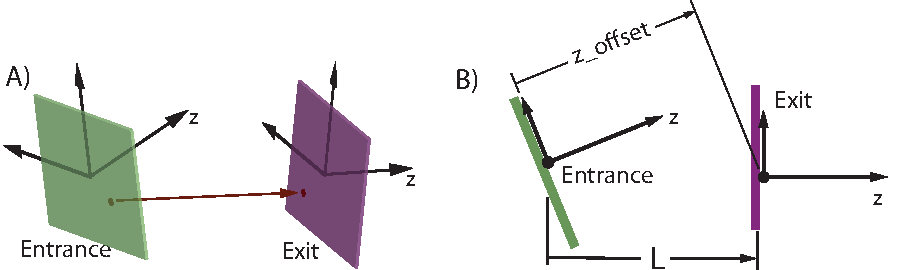
\includegraphics[width=5in]{patch.pdf}
  \caption[Patch Element.]
{A) A \vn{patch} element can align its exit face arbitrarily with respect to its entrance face. The
red arrow illustrates a possible particle trajectory form entrance face to exit face. B) The
reference length of a \vn{patch} element, if \vn{ref_coords} is set to the default value of
\vn{exit_end}, is the longitudinal distance from the entrance origin to the exit origin using the
reference coordinates at the exit end as shown. If \vn{ref_coords} is set to \vn{entrance_end}, the
length of the patch will be equal to the \vn{z_offset}.}
  \label{f:patch}
\end{figure}

%-----------------

A \vn{patch} element shifts the reference orbit and time. Also see \vn{floor_shift}
(\sref{s:floor.ele}) and \vn{fiducial} (\sref{s:fiducial}) elements. A common application of a patch
is to orient two lines with respect to each other. For example, to orient an injection line with the
ring it is injecting into (\sref{s:ex.inj}).

General \vn{patch} element attributes are:
\begin{center}
\tt
\begin{tabular}{llll} \toprule
  {\sl Attribute Class}      & Section           & {\sl Attribute Class}      & Section         \\ \midrule
  Aperture limits            & \ref{s:limit}     & Offsets, pitches \& tilt   & \ref{s:offset}  \\ 
  Chamber wall               & \ref{s:wall}      & Reference energy           & \ref{s:energy}  \\
  Custom Attributes          & \ref{s:cust.att}  & Superposition              & \ref{s:super}   \\
  Description strings        & \ref{s:alias}     & Tracking \& transfer map   & \ref{c:methods} \\
  Length                     & \ref{s:l}         &                            &                 \\
  \bottomrule
\end{tabular}
\end{center}
\toffset
See \sref{s:list.patch} for a full list of element attributes along with a their units.

\index{flexible}\index{e_tot_offset}
\index{x_offset}\index{y_offset}\index{z_offset}\index{tilt}
\index{x_pitch}\index{y_pitch}\index{t_offset}
\index{e_tot_set}\index{p0c_set}
Attributes specific to a \vn{patch} elements are:
\begin{example}
  x_offset        = <Real>    ! Exit face offset from Entrance.
  y_offset        = <Real>    ! Exit face offset from Entrance.
  z_offset        = <Real>    ! Exit face offset from Entrance.
  t_offset        = <Real>    ! Reference time offset.
  x_pitch         = <Real>    ! Exit face orientation from Entrance.
  y_pitch         = <Real>    ! Exit face orientation from Entrance.
  tilt            = <Real>    ! Exit face orientation from Entrance.
  E_tot_offset    = <Real>    ! Reference energy offset (eV).
  E_tot_set       = <Real>    ! Reference energy at exit end (eV).
  flexible        = <T/F>     ! Default: False.
  p0c_set         = <Real>    ! Reference momentum at exit end (eV).
  ref_coords      = <Switch>  ! Coordinate system defining the length.
  user_sets_length = <T/F>    ! User sets element length? Default is F.
  l               = <Real>    ! Reference length. 
\end{example}
\index{x_offset}

A straight line element like a \vn{drift} or a \vn{quadrupole} has the exit face parallel to the
entrance face. With a \vn{patch} element, the entrance and exit faces can be arbitrarily oriented
with respect to one another as shown in \fig{f:patch}A.

\index{rigid patch}\index{inflexible patch}
\index{flexible patch}
There are two different ways the orientation of the exit face is determined. Which way is used is
determined by the setting of the \vn{flexible} attribute.  With the \vn{flexible} attribute set to
\vn{False}, the default, The exit face of the \vn{patch} will be determined from the offset, tilt
and pitch attributes as described in \sref{s:patch.coords}. This type of \vn{patch} is called
``rigid'' or ``inflexible'' since the geometry of the \vn{patch} is solely determined by the
\vn{patch}'s attributes as set in the lattice file and is independent of everything else. Example:
\begin{example}
  pt: patch, z_offset = 3.2   ! Equivalent to a drift
\end{example}

With \vn{flexible} set to \vn{True}, the exit face is taken to be the reference frame of the
entrance face of the next element in the lattice. In this case, it must be possible to compute the
reference coordinates of the next element before the reference coordinates of the \vn{patch} are
computed. A \vn{flexible} \vn{patch} will have its offsets, pitches, and tilt as dependent
parameters (\sref{s:depend}) and these parameters will be computed appropriately. Here the
\vn{patch} is called ``flexible'' since the geometry of the patch will depend upon the geometry of
the rest of the lattice and, therefore, if the geometry of the rest of the lattice is modified (is
``flexed''), the geometry of the \vn{patch} will vary as well. See Section~\sref{s:ex.erl} for an
example.

The coordinates of the lattice element downstream of a \vn{flexible} \vn{patch} can be computed
if there is a \vn{fiducial} element (\sref{s:fiducial}) somewhere downstream or if there is a
\vn{multipass_slave} (\sref{s:multipass}) element which is just downstream of the \vn{patch} or at
most separated by zero length elements from the \vn{patch}. In this latter case, the
\vn{multipass_slave} must represent an $N$\Th pass slave with $N$ greater than 1. This works since
the first pass slave will be upstream of the \vn{patch} and so the first pass slave will have its
coordinates already computed and the position of the downstream slave will be taken to be the same
as the first pass slave. Notice that, without the \vn{patch}, the position of multipass slave
elements are independent of each other.

With \vn{bmad_standard} tracking (\sref{s:tkm}) A particle, starting at the upstream face of the
\vn{patch}, is propagated in a straight line to the downstream face and the suitable coordinate
transformation is made to translate the particle's coordinates from the upstream coordinate frame to
the downstream coordinate frame (\sref{s:patch.std}). In this case the \vn{patch} element can be
thought of as a generalized \vn{drift} element.

If there are magnetic or electric fields within the \vn{patch}, the tracking method through the
\vn{patch} must be set to either \vn{runge_kutta} or \vn{custom}. Example:
\begin{example}
  pa2: patch, tracking_method = runge_kutta, field_calc = custom, 
              mat6_calc_method = tracking, ...
\end{example}
In order to supply a custom field when \vn{runge_kutta} tracking is used, \vn{field_calc}
(\sref{s:integ}) needs to be set to \vn{custom}. In this case, custom code must be supplied for
calculating the fields as a function of position (\sref{s:custom.ele}).

The \vn{E_tot_offset} attribute offsets the
reference energy:
\begin{example}
  E_tot_ref(exit) = E_tot_ref(entrance) + E_tot_offset (eV)
\end{example}
Setting the \vn{E_tot_offset} attribute will affect a particle's $p_x$, $p_y$ and $p_z$ coordinates
via \Eqs{ppp} and \eq{ppppp}.  Notice that \vn{E_tot_offset} does not affect a particle's actual
energy, it just affects the difference between the particle energy and the reference energy.

Alternatively, to set the reference energy, the \vn{E_tot_set} or \vn{p0c_set} attributes can be
used to set the reference energy/momentum at the exit end. It is is an error if more than one of
\vn{E_tot_offset}, \vn{E_tot_set} and \vn{p0c_set} is nonzero.

\vn{Important}: \bmad may apply the energy transformation either before or after the coordinate
transformation. This matters when the speed of the reference particle is less than $c$. For this
reason, and due to complications involving PTC, it is recommended to use two patches in a row when
both the orbit and energy are to be patched.

A \vn{patch} element can have an associated electric or magnetic field (\sref{s:fieldmap}). This can
happen, for example, if a patch is used at the end of an injection line to match the reference
coordinates of the injection line to the line being injected into (\sref{s:ex.inj}) and the patch
element is within the field generated by an element in the line being injected into. In such a case,
it can be convenient to set what the reference coordinates are since the orientation of any fields
that are defined for a patch element will be oriented with respect to the patch element's reference
coordinates. For this, the \vn{ref_coords}
parameter of a patch can be used. Possible settings are:
\vn{ref_coords} are:
\begin{example}
  entrance_end  !
  exit_end      ! Default
\end{example}
The default setting of \vn{ref_coords} is \vn{exit_end} and with this the reference coordinates are
set by the exit end coordinate system (see \fig{f:patch}). If \vn{ref_coords} is set to
\vn{entrance_end}, the reference coordinates are set by the entrance end coordinate system. Example:
\begin{example}
  p1: patch, x_offset = 1, x_pitch = 0.4   ! L = 0.289418 see below
  p2: p1, ref_coords = entrance_end        ! L = 0
\end{example}
Here \vn{p1} has \vn{ref_coords} set to \vn{exit_end} (the default). \vn{p2} inherits the parameters
of \vn{p1} and sets \vn{ref_coords} to \vn{entrance_end}.

It is important to keep in mind that if there are multiple patches in a row, while two different
configurations may be the same in a geometrical sense the total length may not be the same. For
example:
\begin{example}
  pA: patch, x_offset = 1    ! L = 0
  pB: patch, x_pitch = 0.4   ! L = 0
  sum: line = (pA, pB)
\end{example}
The configuration of \vn{pA} followed by \vn{pB} is equivalent geometrically to the \vn{p1} patch
above but the total length of the \vn{(pA, pB)} line is zero which is different from the length of
\vn{p1}.

Unfortunately, there is no intuitive way to define the ``\vn{length}'' \vn{L} of a patch. This is
important since the transit time of the reference particle is the element length divided by the
reference velocity. And the reference transit time will affect how the phase space $z$ coordinate
changes through the patch via \Eq{zbctt}. If the parameter \vn{user_sets_length} is set to True, the
value of \vn{l} set in the lattice file will be used (default is zero). \vn{user_sets_length} is set
to False (the default), the length of a patch is calculated depending upon the setting of
\vn{ref_coords}.  If \vn{ref_coords} is set to \vn{exit_end}, the length of the patch is calculated
as the perpendicular distance between the origin of the patch's entrance coordinate system and the
exit face of the patch as shown in \fig{f:patch}B. If \vn{ref_coords} is set to \vn{entrance_end},
the length is calculated as the perpendicular distance between the entrance face and the origin of
the exit coordinate system. In this case, the length will be equal to \vn{z_offset}.

To provide flexibility, the \vn{t_offset} attribute can be
used to offset the reference time. The reference time at the exit end of the patch
\vn{t_ref(exit)} is related to the reference time at the beginning of the patch \vn{t_ref(entrance)}
via
\begin{example}
  t_ref(exit) = t_ref(entrance) + t_offset + dt_travel_ref
\end{example}
where \vn{dt_travel_ref} is the time for the reference particle to travel through the patch.
\vn{dt_travel_ref} is defined to be:
\begin{example}
  dt_travel_ref = L / beta_ref
\end{example}
Where \vn{L} is the length of the \vn{patch} and \vn{beta_ref} is the reference velocity/c at the
exit end of the element. That is, the reference energy offset is applied {\em before} the reference
particle is tracked through the patch. Since this point can be confusing, it is recommended that a
\vn{patch} element be split into two consecutive patches if the \vn{patch} has finite \vn{l} and
\vn{E_tot_offset} values.

While a finite \vn{t_offset} will affect the reference time at the end of a patch, a finite
\vn{t_offset} will {\em not} affect the time that is calculated for a particle to reach the end of
the patch. On the other hand, a finite \vn{t_offset} will affect a particle's $z$ coordinate via
\Eqs{zbctt}. The change in $z$, $\delta z$ will be
\begin{equation}
  \delta z = \beta \cdot c \cdot \text{t_offset}
\end{equation}
where $\beta$ is the normalized particle speed (which is independent of any energy patch). Another
way of looking at this is to note that In a drift, if the particle is on-axis and on-energy, t and
t_ref change but z does not change. In a time patch (a patch with only \vn{t_offset} finite), t_ref
and z change but t does not.

When a lattice branch contains both normally oriented and reversed elements
(\sref{s:ref.construct}), a \vn{patch}, or series of \vn{patches}, which reflects the $z$ direction
must be placed in between. Such a \vn{patch}, (or patches) is called a \vn{reflection} \vn{patch}.
See Section~\sref{s:reflect.patch} for more details on how a reflection patch is defined. In order
to avoid some confusing conceptual problems involving the coordinate system through a reflection
patch, Runge-Kutta type tracking is prohibited with a reflection patch.\footnote
  {
In general, Runge-Kutta type tracking through a patch is a waste of time unless electric or magnetic
fields are present.
  }

\index{wall}
Since the geometry of a \vn{patch} element is complicated, interpolation of the chamber wall in the
region of a patch follows special rules. See section~\sref{s:wall.vacuum} for more details.

\newpage

%-----------------------------------------------------------------
\section{Photon_Init}
\label{s:photon.init}
\index{photon_init|hyperbf}

A \vn{photon_init} element is used as a starting element for x-ray tracking.  A \vn{photon_init}
element can be used to define such things as the initial energy spectrum and angular orientation. As
explained below, a \vn{photon_init} element can be a ``stand alone'' photon source or it can have an
associated ``physical source'' element.

Note: There is a utility program called \vn{photon_init_plot} that comes with a Bmad Distribution
that will plot initial photon distributions and can be used as a check.

General \vn{photon_init} attributes are:
\begin{center}
\tt
\begin{tabular}{llll} \toprule
  {\sl Attribute Class}      & Section           & {\sl Attribute Class}      & Section         \\ \midrule
  Aperture limits            & \ref{s:limit}     & Length                     & \ref{s:l}       \\
  Chamber wall               & \ref{s:wall}      & Offsets, pitches \& tilt   & \ref{s:offset}  \\
  Custom Attributes          & \ref{s:cust.att}  & Reference energy           & \ref{s:energy}  \\ 
  Description strings        & \ref{s:alias}     & Tracking \& transfer map   & \ref{c:methods} \\ 
  \bottomrule
\end{tabular}
\end{center}
\toffset
See \sref{s:list.photon.init} for a full list of element attributes along with a their units.

\index{x_half_length}\index{y_half_length}
Attributes specific to an \vn{photon_init} element are:
\begin{example}
  ds_slice                 = <Real>
  E_center                 = <Real>    ! Average init photon energy of 1st mode (eV).
  E2_center                = <Real>    ! Average init photon energy of 2nd mode (eV).
  E2_probability           = <Real>    ! Probability of 2nd mode.
  E_center_relative_to_ref = <T/F>     ! E_center relative to reference E? Default True.
  e_field_x                = <Real>    ! Polarization. x & y = 0 -> random
  e_field_y                = <Real>
  energy_distribution      = <Switch>  ! Gaussian, uniform, or curve.
  energy_probability_curve = \{...\}   ! Used with energy_distribution = curve. See below.
  physical_source          = <String>  ! physical source of x-rays
  ref_wavelength                       ! Ref wavelength (\sref{s:energy}). Dep attribute (\sref{s:depend}).
  sig_x                    = <Real>
  sig_y                    = <Real>
  sig_z                    = <Real>
  sig_vx                   = <Real>
  sig_vy                   = <Real>
  sig_E                    = <Real>    ! Init photon energy width of 1st mode (eV).
  sig_E2                   = <Real>    ! Init photon energy width of 2nd mode (eV).
  spatial_distribution     = <Switch>  ! Gaussian or uniform. 
  transverse_sigma_cut     = <Real>
  velocity_distribution    = <Switch>  ! Gaussian, spherical, or uniform. 
\end{example}

When the \vn{energy_distribution} is set to \vn{gaussian} or \vn{uniform}, the distribution of
photons is bimodal. The first mode is characterized by the parameters \vn{E_center}, and \vn{sig_E},
the second mode is characterized by the parameters \vn{E2_center} and \vn{sig_E2}. The probability
of emitting a photon in the second mode is given by \vn{E2_probability}.

\begin{description}
%
  \index{ds_slice}
  \item[\vn{ds_slice}] \Newline
Used when there is an associated physical source element. The physical source element is sliced into
pieces of thickness \vn{ds_slice} and each slice is tested to see if photons from the slice can
possibly pass through the first aperture. When photons are generated, photons will only be generated
from slices where they have a hope of passing through the first aperture. This makes the simulation
more efficient.  The default value of \vn{ds_slice} is 0.01 meter.
%
  \index{E_center}\index{E2_center}
  \item[\vn{E_center}, \vn{E2_center}] \Newline
Average initial photon energy in eV. If \vn{E_center_relative_to_ref} is set to True, \vn{E_center}
and \vn{E2_center} will be relative to the reference energy.
%
  \index{E_center_relative_to_ref}
  \item[\vn{E_center_relative_to_ref}] \Newline
With a setting of True (the default), \vn{E_center} and \vn{E2_center} are taken to be with respect
to the reference energy (\sref{s:ref.energy}). That is, if True, the center energy \vn{<E>} is
\begin{example}
  <E-1st-mode> = E1_center + Reference_Energy
  <E-2nd-mode> = E2_center + Reference_Energy
\end{example}
If \vn{E_center_relative_to_ref} is set to False, \vn{E_center} and \vn{E2_center} are taken to be
the center energy values independent of the reference energy.
%
  \index{E2_probability}
  \item[\vn{E2_probability}] \Newline
Probability of emitting a photon from the 2nd mode. A value of 0 (the default) will mean
that all photons will be emitted from the 1st mode and a value of 1 will mean that
all photons will be emitted from the 2nd mode.
%
  \index{e_field_x}\index{e_field_y}
  \item[\vn{e_field_x}, \vn{e_field_y}] \Newline
Electric field component of initial photons in the $x$ and $y$ planes. If both are set to 0 then a
random field is chosen with unit intensity $E_x^2 + E_y^2 = 1$.
%
  \index{energy_distribution}
  \item[\vn{energy_distribution}] \Newline
Sets the type of energy spectrum for emitted photons. If there is an associated physical element
then this parameter is ignored and the energy distribution is calculated from the properties of the
physical element. Possible settings are:
\begin{example}
  gaussian   ! Default
  uniform
  curve
\end{example}
The \vn{gaussian} setting gives Gaussian distributions for the two modes with width set by
\vn{sig_E} and \vn{sig_E2}. The \vn{uniform} setting gives a flat distribution in the range:
\begin{example}
  [-sig_E, sig_E]    ! For the 1st mode
  [-sig_E2, sig_E2]  ! For the 2nd mode
\end{example}
The \vn{curve} setting uses the energy probability curve set by the \vn{energy_probability_curve}
component.
%
  \index{energy_probability_curve}
  \item[\vn{energy_probability_curve}] \Newline
The \vn{energy_probability_curve} attribute provides a way to specify the energy probability
distribution when an Gaussian or uniform distribution is not suitable. The probability curve is
defined by specifying the curve at a number of points. The syntax is:
\begin{example}
  energy_probability_curve = \{E1 p1, E2 p2, ..., EN pN\}
\end{example}
where the \vn{E p} pairs are the energy and photon emissian probability at that energy. 
The commas between \vn{E p} pairs is optional.
The probability curve does not have to be normalized, \bmad will take care of that. \bmad will
use cubic spline interpolation between points. 
%
  \index{physical_source}
  \item[\vn{physical_source}] \Newline
Used to specify the ``physical'' source of the photons. See below for more details
%
  \index{sig_E}\index{sig_E2}
  \item[\vn{sig_E}, \vn{sig_E2}] \Newline
Energy width of the two modes in eV. See \vn{energy_distribution} for more details.
%
  \index{sig_vx}\index{sig_vy}
  \item[\vn{sig_vx, sig_vy}] \Newline
Width of emitted photons in $v_x/c$ and $v_y/c$ directions. See
\vn{velocity_distribution} for more details.
%
  \index{sig_x}\index{sig_y}\index{sig_z}
  \item[\vn{sig_x, sig_y, sig_z}] \Newline
Width of emitted photons in $x$, $y$ and $z$ directions. See
\vn{spatial_distribution} for more details.
%
  \index{spatial_distribution}
  \item[\vn{spatial_distribution}] \Newline
Sets spacial $(x, y, z)$ spectrum of emitted photons. If there is an associated physical element
then this parameter is ignored and the energy distribution is calculated from the properties of the
physical element. Possible settings are:
\begin{example}
  gaussian    ! Default
  uniform
\end{example}
The \vn{gaussian} setting gives a Gaussian distribution with width
$\sigma$ where $\sigma$ is 
\begin{example}
  sig_x     ! for x distribution
  sig_y     ! for y distribution
  sig_z     ! for z distribution
\end{example}
The \vn{uniform} setting gives a flat
distribution in the range: $[-\sigma, \sigma]$.
%
  \index{velocity_distribution}
  \item[\vn{velocity_distribution}] \Newline
Sets the transverse $(v_x/c, v_y/c)$ velocity spectrum of emitted photons. If there is an associated
physical element then this parameter is ignored and the energy distribution is calculated from the
properties of the physical element. The longitudinal velocity is always computed to make $v_x^2 +
v_y^2 + v_z^2 = c^2$ Possible settings are:
\begin{example}
  gaussian    ! Default
  spherical
  uniform
\end{example}
The \vn{gaussian} setting gives a Gaussian distribution with width
$\sigma$ where $sigma$ is 
\begin{example}
  sig_vx     for vx/c distribution
  sig_vy     for vy/c distribution
\end{example}
The \vn{uniform} setting gives a flat distribution in the range: $[-\sigma, \sigma]$. The
\vn{spherical} setting gives flat distribution in all directions. With the \vn{spherical}
setting is used, and the next downstream element excluding drifts and markers is an element
with aperture limits (\sref{s:limit}), \bmad can optimize photon emission to only emitting 
photons that are very likely to be within the aperture when they hit the downstream element.
This cuts down on computation time.
%
\end{description}

For the purposes of positioning the elements in the lattice around it,
a \vn{photon_init} element is considered to have zero length.

\vn{photon_init} elements are used in one of two modes: With or without an associated physical
source element specified by the \vn{physical_source} attribute. Without an associated physical
source, the \vn{photon_init} element completely specifies the initial photon distribution. With an
associated physical source element, the photon distribution is determined by the properties of the
physical source but the shape of the energy spectrum can be modified by setting attributes in the
\vn{photon_init} element. Example:
\begin{example}
  b05w: sbend, l = 3.2, angle = 0.1
  pfork: photon_fork, to_line = c_line, superimpose, ref = b05w, offset = 0.4
  bend_line: line = (..., b05w, ...)
  use bend_line

  c_line: line = (pinit, ...)
  c_line[E_tot] = 15e3
  pinit: photon_init, physical_source = "b05w", sig_E = 2.1
\end{example}
In this example, the bend \vn{b05w} is a bend producing photons. It is part of the line
\vn{bend_line}. \vn{bend_line} also contains a \vn{photon_fork} element named \vn{pfork} which
branches to the line \vn{c_line}. \vn{c_line} contains the \vn{photon_init} element \vn{pinit} which
references \vn{b03w} as the associated physical source element. When photons are tracked, they are
generated in \vn{b05w} and then propagated to the \vn{pfork} fork.  After this they are propagated
through \vn{c_line}. The \vn{pinit} element acts like a zero length \vn{marker} element when photons
propagate through it. That is, the \vn{pinit} element essentially serves to associate \vn{c_line}
with \vn{b03w} for the purposes of photon tracking. Also, in this example, \vn{pinit} modifies the
photon energy spectrum so that only photons whose energy is within 2.1 eV are generated

It is important to note that in the above example, with the \vn{photon_init} element having an
associated physical source, the setting of things like the spatial shape \vn{sig_z}, etc. in the
\vn{photon_init} element will be ignored.

See Section~\sref{s:rowland} for an example lattice that can be used to simulate a Rowland circle
spectrometer using a \vn{photon_init} element.

\newpage

%-----------------------------------------------------------------
\section{Quadrupole}
\label{s:quad}
\index{quadrupole|hyperbf}

A \vn{quadrupole} is a magnetic element with a linear field dependence
with transverse offset (\sref{s:mag.field}).

General \vn{quadrupole} attributes are:
\begin{center}
\tt
\begin{tabular}{llll} \toprule
  {\sl Attribute Class}      & Section           & {\sl Attribute Class}      & Section            \\ \midrule
  Aperture limits            & \ref{s:limit}     & Mag \& Elec multipoles     & \ref{s:multip}     \\
  Chamber wall               & \ref{s:wall}      & Offsets, pitches \& tilt   & \ref{s:offset}     \\
  Description strings        & \ref{s:alias}     & Overlapping Fields         & \ref{s:overlap}    \\
  Fringe Fields              & \ref{s:fringe}    & Reference energy           & \ref{s:energy}     \\ 
  Hkick \& Vkick             & \ref{s:kick}      & Superposition              & \ref{s:super}      \\
  Integration settings       & \ref{s:integ}     & Symplectify                & \ref{s:symp}       \\
  Is_on                      & \ref{s:is.on}     & Field Maps                 & \ref{s:fieldmap}   \\ 
  Length                     & \ref{s:l}         & Tracking \& transfer map   & \ref{c:methods}    \\ 
  \bottomrule
\end{tabular}
\end{center}
\toffset
See \sref{s:list.quadrupole} for a full list of element attributes along with a their units.

\index{f1}\index{f2}
\index{k1}\index{b1_gradient}
Attributes specific to a \vn{quadrupole} element are:
\begin{example}
  b1_gradient  = <Real>    ! Field strength. (\sref{s:depend}).
  k1           = <Real>    ! Quadrupole strength.
  fq1          = <Real>    ! Soft edge fringe parameter.
  fq2          = <Real>    ! Soft edge fringe parameter.
  field_master = <T/F>     ! See \sref{s:field.master}.
 \end{example}
The normalized quadrupole \vn{k1} strength is related to the unnormalized \vn{b1_gradient} field
strength through \Eq{kqlbp}.

\index{tilt}
If the \vn{tilt} attribute is present without a value then a value of $\pi/4$
is used.

For a quadrupole with zero \vn{tilt} and a positive \vn{k1}, the
quadrupole is horizontally focusing and vertically defocusing
(\sref{s:mag.field}).

The \vn{fq1} and \vn{fq2} parameters are used to specify the
quadrupolar ``soft'' edge fringe. See \sref{s:q.soft} for more details.
The \vn{fringe_at} and \vn{fringe_type} settings (\sref{s:fringe})
determine if the fringe field is used in tracking (\sref{s:fringe}).

Example:
\begin{example}
  q03w: quad, l = 0.6, k1 = 0.003, tilt  ! same as tilt = pi/4
\end{example}

\newpage

%-----------------------------------------------------------------------------
\section{Ramper}
\label{s:ramper}
\index{ovlerlay|hyperbf}

A \vn{ramper} element is a type of \vn{control} element (\sref{s:lord.slave}). That is, a
\vn{ramper} element can be used to make variations in the attributes of other elements while a
program is running. The \vn{ramper} element is similar to an \vn{overlay} element except that
\vn{ramper} elements are designed to control large sets of elements. Also \vn{ramper} elements can
be used to smoothly vary parameters as particle are propagated through a lattice. \vn{Ramper}
elements where implemented to solve the problem of simulating machine ramping where the strength of
many elements in a machine are varied continuously as a function of time. The drawback of
\vn{ramper} elements is that they can be only be used with programs that that are designed to handle
them.\footnote
  {
In particular, the \vn{long_term_tracking} program that is bundled with the \bmad software
(\sref{s:tao.intro}) can handle \vn{ramper} elements.
  }
Ramper elements will be ignored in programs that are not designed to handle them. How a program
handles ramper elements will be program dependent and the program documentation should be consulted
for details.

Note: \vn{ac_kicker} elements can also be used for simulating a time dependent element.

General \vn{ramper} attributes are:
\begin{center}
\tt
\begin{tabular}{llll} \toprule
  {\sl Attribute Class}      & Section           & {\sl Attribute Class}      & Section         \\ \midrule
  Custom Attributes          & \ref{s:cust.att}  & Is_on                      & \ref{s:is.on}   \\
  Description strings        & \ref{s:alias}     &                            &                 \\ 
  \bottomrule
\end{tabular}
\end{center}
\toffset
See \sref{s:list.ramper} for a full list of element attributes.

The syntax for \vn{ramper} elements is exactly the same as for \vn{overlay} (\sref{s:go.syntax}) elements 
except that \vn{ramper} elements do not have a \vn{gang} attribute.

Like \vn{overlay}s, There are two types of \vn{ramper} elements: \vn{Expression} based and
\vn{knot} based.  The general syntax for a \vn{expression} based \vn{ramper} element is
\begin{example}
  name: RAMPER = \{ele1[attrib1]:coef1, ele2[attrib2]:coef2, ...\}, VAR = \{var1\}
\end{example}
where \vn{ele1[attrib1]}, \vn{ele2[attrib2]}, etc. specify the slave attributes and \vn{exp1},
\vn{exp2}, etc. are the arithmetical expressions, that are functions of \vn{var1}, \vn{var2}, etc.,
and are used to determine a value for the slave attributes.

The general syntax for a \vn{knot} based  \vn{ramper} element is
\begin{example}
  name: RAMPER = \{ele1[attrib1]:\{y_knot_points1\}, ele2[attrib2]:\{y_knot_points2\}, ...\}, 
              VAR = \{var1\}, X_KNOT = \{x_knot_points\}, INTERPOLATION = \{type\},
              var1 = init_val1, ...
\end{example}

\textbf{See Section~\sref{s:go.syntax} for a detailed description of this syntax.}

Examples:
\begin{example}
  ramp_e: ramper = \{*[e_tot]:\{4e+08, 4.00532e+08, 4.01982e+08, ...\}\},
                var = \{time\}, x_knot = \{0, 0.001, 0.002, ...\}, interpolation = cubic

  amp = 1e9;  omega = 0.167;  t0 = 0.053
  ramp_rf: ramper = \{rfcavity::*[voltage]:amp*sin(omega *(t + t0)),
        rfcavity::*[phi0]:0.00158*t^2 + 3*q\}, var = \{t, q\}
\end{example}
\vn{Ramp_e} uses a cubic spline fit to interpolate between the knot points specified in the element
definition.  The ``\vn{*[e_tot]}'' construct in the definition of \vn{ramp_e} means that the ramper
will be applied to the \vn{e_tot} attribute (\sref{s:energy}) of all elements (since the wild card
character ``\vn{*}'' (\sref{s:ele.match}) will match to all element names).

The \vn{ramp_rf} ramper in the above example varies the \vn{voltage} and \vn{phase} (\vn{phi0})
attributes of all elements that match to \vn{rfcavity::*}. That is, all \vn{rfcavity} elements. Here
mathematical expressions are used instead of knot points.

\vn{Ramper} elements can control the variables of other controller element but in this case it is
not permitted to use wild card characters. That is, in the above example, ``\vn{*}'' will not match
to any controller elements.

Unlike \vn{group} or \vn{overlay} elements, it is not permitted for different \vn{ramper} elements
to control the same parameter of a given slave element. Additionally, parameters that \vn{ramper}
elements control must not be controlled by any \vn{overlay}.

Note: There is a program to plot controller response curves bundled with the \bmad software
(\sref{s:tao.intro}) called \vn{controller_function_plot}. Documentation on this can
be found at:
\begin{example}
  util_programs/controller_function_plot
\end{example}

\newpage

%-----------------------------------------------------------------
\section{RF_bend}
\label{s:rf.bend}
\index{rf_bend|hyperbf}

An \vn{rf_bend} is an RF cavity with the geometry of an \vn{sbend} (\sref{s:bend}). This element is
currently considered to be experimental so please contact a \bmad maintainer if you want to use this
type of element.

General \vn{rfcavity} attributes are:
\begin{center}
\tt
\begin{tabular}{llll} \toprule
  {\sl Attribute Class}      & Section            & {\sl Attribute Class}      & Section            \\ \midrule
  Aperture limits            & \ref{s:limit}      & Offsets, pitches \& tilt   & \ref{s:offset}     \\
  Chamber wall               & \ref{s:wall}       & Overlapping Fields         & \ref{s:overlap}    \\
  Custom Attributes          & \ref{s:cust.att}   & Reference energy           & \ref{s:energy}     \\ 
  Description strings        & \ref{s:alias}      & Superposition              & \ref{s:super}      \\
  Symplectify                & \ref{s:symp}       & Field Maps                 & \ref{s:fieldmap}   \\
  Integration settings       & \ref{s:integ}      & Tracking \& transfer map   & \ref{c:methods}    \\
  Is_on                      & \ref{s:is.on}      & Wakes                      & \ref{s:wakes}      \\
  Length                     & \ref{s:l}          &                            &                    \\
  \bottomrule
\end{tabular}
\end{center}
\toffset
See \sref{s:list.rf.bend} for a full list of element attributes along with a their units.

\index{rf_frequency}\index{harmon}\index{voltage}\index{phi0}\index{phi0_multipass}
Attributes specific to an \vn{rf_bend} are:
\begin{example}
  ! Bend-like attributes:
  angle              = <Real>   ! Design bend angle. Settable dependent var (\sref{s:depend}).
  b_field            = <Real>   ! Design field strength (= P_0 g / q) (\sref{s:depend}).
  g                  = <Real>   ! Design bend strength (= 1/rho).
  l                  = <Real>   ! "Length" of bend. See below.
  l_arc              = <Real>   ! Arc length. For \vn{rbend}s only. 
  l_chord            = <Real>   ! Chord length. See \sref{s:l}.
  l_sagitta                     ! Sagittal length. Dependent param (\sref{s:depend}).
  rho                = <Real>   ! Design bend radius. Settable dependent param (\sref{s:depend}).
  roll               = <Real>   ! See \ref{s:offset}.
  field_master       = <T/F>    ! See \ref{s:field.master}.

  ! RF-like attributes:
  rf_frequency    = <Real>    ! Frequency
  harmon          = <Real>    ! Harmonic number
  phi0            = <Real>    ! Cavity phase (rad/2pi).
  phi0_multipass  = <Real>    ! Phase variation with multipass (rad/2pi).
\end{example}

Tracking through an \vn{rf_bend} is limited to Runge Kutta like tracking methods (\sref{s:tkm}). The
default \vn{tracking_method} is \vn{runge_kutta}. Fields must be specified using a grid field map
(\sref{s:fieldmap}). The default \vn{field_calc} is \vn{fieldmap} (\sref{s:field.calc}).

The geometry of the \vn{rf_bend} is the same as an \vn{sbend}. An \vn{rf_bend} has a sector shape
which is equivalent to \vn{e1} and \vn{e2} being zero for an \vn{sbend}. Since the fields are specified
using a grid field map, there are no fringe attributes to set (for any elements where a grid field is
used, it is always assumed that the fringe fields are included as part of the grid field).

\newpage

%-----------------------------------------------------------------
\section{RFcavity}
\label{s:rfcav}
\index{rfcavity|hyperbf}

An \vn{rfcavity} is an RF cavity without acceleration generally used in a storage ring. The main
difference between an \vn{rfcavity} and an \vn{lcavity} is that, unlike an \vn{lcavity}, the
reference energy (\sref{s:phase.space}) through an \vn{rfcavity} is constant.

General \vn{rfcavity} attributes are:
\begin{center}
\tt
\begin{tabular}{llll} \toprule
  {\sl Attribute Class}      & Section            & {\sl Attribute Class}      & Section            \\ \midrule
  Aperture limits            & \ref{s:limit}      & Offsets, pitches \& tilt   & \ref{s:offset}     \\
  Chamber wall               & \ref{s:wall}       & Overlapping Fields         & \ref{s:overlap}    \\
  Custom Attributes          & \ref{s:cust.att}   & Reference energy           & \ref{s:energy}     \\ 
  Description strings        & \ref{s:alias}      & RF Couplers                & \ref{s:rf.coupler} \\
  Field autoscaling          & \ref{s:autoscale}  & Superposition              & \ref{s:super}      \\
  Fringe Fields              & \ref{s:fringe}     & Symplectify                & \ref{s:symp}       \\
  Hkick \& Vkick             & \ref{s:kick}       & Field Maps                 & \ref{s:fieldmap}   \\
  Integration settings       & \ref{s:integ}      & Tracking \& transfer map   & \ref{c:methods}    \\
  Is_on                      & \ref{s:is.on}      & Wakes                      & \ref{s:wakes}      \\
  Length                     & \ref{s:l}          &                            &                    \\
  \bottomrule
\end{tabular}
\end{center}
\toffset
See \sref{s:list.rfcavity} for a full list of element attributes along with a their units.

\index{rf_frequency}\index{harmon}\index{voltage}\index{phi0}\index{phi0_multipass}
Attributes specific to an \vn{rfcavity} are:
\begin{example}
  rf_frequency    = <Real>    ! Frequency
  harmon          = <Real>    ! Harmonic number
  voltage         = <Real>    ! Cavity voltage
  phi0            = <Real>    ! Cavity phase (rad/2pi).
  phi0_multipass  = <Real>    ! Phase variation with multipass (rad/2pi).
  phi0_autoscale  = <Real>    ! Set by Bmad if autoscaling is turned on (rad/2pi).
  gradient        = <Real>    ! Accelerating gradient (V/m). Dependent attribute (\sref{s:depend}).
  longitudinal_mode = <Int>   ! Longitudinal mode. Default is 1. May be 0 or 1.
\end{example}

The integrated energy kick felt by a particle, assuming no phase slippage, is 
\begin{example}
  dE = -e_charge * \(r_q\) * voltage * sin(\(2\,\pi\) * (\(\phi_\text{t}\) - \(\phi_\REF\)))
\end{example}
\index{multipass}
where
\begin{example}
  \(\phi_\REF\) = phi0 + phi0_multipass + phi0_autoscale
  \label{rfcav.phi}
\end{example}
and $\phi_t$ is the part of the phase due to when the particle arrives at the cavity and depends
upon whether \vn{absolute time tracking} or \vn{relative time tracking} is being used as discussed
in \sref{s:rf.time}.

In the above equation $r_q$ is the relative charge between the reference particle (set by the
\vn{parameter[particle]} parameter in a lattice file) and the particle being tracked through the
cavity. For example, if the reference particle and and the tracked particle are the same, $r_q$ is
unity independent of the type of particle tracked.

The correspondence between the \bmad \vn{phi0} attribute and the \vn{lag} attribute of
\mad is
\begin{example}
  phi0 = mad + 0.5
\end{example}

\vn{phi0_multipass} is only to be used to shift the phase with respect to a \vn{multipass} lord. See
\sref{s:multipass}. \vn{e_charge} is the magnitude of the charge on an electron
(Table~\ref{t:constants}). Notice that the energy kick is independent of the sign of the charge of
the particle

\vn{phi0_autoscale} and \vn{field_autoscale} are calculated by \bmad's auto-scale module. See
Section~\sref{s:autoscale} for more details. Autoscaling can be toggled on/off by using the
\vn{autoscale_phase} and \vn{autoscale_amplitude} toggles.

Note: Zero phase for $\phi_\REF$ corresponds to the stable fixed point above transition.

If \vn{harmon} is non--zero the \vn{rf_frequency} is calculated by
\begin{example}
  rf_frequency = harmon * c_light * beta0 / L_lattice 
\end{example}
where \vn{L_lattice} is the total lattice length and \vn{beta0} is the
velocity of the reference particle at the start of the lattice. After
the lattice has been read in, \vn{rf_frequency} will be the
independent variable (\sref{s:depend}).

Couplers (\sref{s:rf.coupler}) and HOM wakes (\sref{s:wakes}) can
be modeled. In addition, if a field map is specified
(\sref{s:fieldmap}), tracking using an integrator is possible.

\index{RF field map}
\index{runge_kutta!and field maps}
\index{symp_lie_bmad!and field maps}
If a field map is specified (\sref{s:fieldmap}), tracking using an integrator is possible. A field
map is only used for \vn{runge_kutta}, \vn{fixed_step_runge_kutta}, and \vn{symp_lie_bmad} tracking
(\sref{s:tkm}). Only the fundamental mode has an analytical formula for the symplectic
tracking. With \vn{cavity_type} set to \vn{standing_wave}, the longitudinal mode is set by the
\vn{longitudinal_mode} parameter. The possible values are 0 or 1 and the default setting is 0.

The \vn{cavity_type} is the type of cavity being simulated. Possible
settings are:
\begin{example}
  ptc_standard
  standing_wave    ! Default
  traveling_wave
\end{example}
The \vn{cavity_type} switch is ignored if a field map is used.

Example:
\begin{example}
  rf1: rfcav, l = 4.5, harmon = 1281, voltage = 5e6
\end{example}

\newpage

%-----------------------------------------------------------------
\section{Sad_Mult}
\label{s:sad.mult}
\index{sad_mult|hyperbf}

A \vn{sad_mult} element is equivalent to a SAD\cite{b:sad} \vn{mult}
element. This element is a combination solenoid, multipole, bend, and
RF cavity.

General \vn{sample} attributes are:
\begin{center}
\tt
\begin{tabular}{llll} \toprule
  {\sl Attribute Class}      & Section           & {\sl Attribute Class}      & Section         \\ \midrule
  a$n$, b$n$ multipoles      & \ref{s:multip}    & Length                     & \ref{s:l}       \\
  Aperture limits            & \ref{s:limit}     & Offsets, pitches \& tilt   & \ref{s:offset}  \\
  Chamber wall               & \ref{s:wall}      & Reference energy           & \ref{s:energy}  \\ 
  Custom Attributes          & \ref{s:cust.att}  & Superposition              & \ref{s:super}   \\
  Description strings        & \ref{s:alias}     & Tracking \& transfer map   & \ref{c:methods} \\ 
  Fringe Fields              & \ref{s:fringe}    &                            &                 \\
  \bottomrule
\end{tabular}
\end{center}
\toffset
See \sref{s:list.sad.mult} for a full list of element attributes along with a their units.

\index{angle}\index{bs_field}\index{e1}\index{e2}\index{eps_step_scale}
\index{f1}\index{f2}\index{g}\index{rf_frequency}\index{harmon}
\index{ks}\index{phi0}\index{rho}\index{voltage}\index{x_offset_mult}
\index{y_offset_mult}\index{x_pitch_mult}\index{y_pitch_mult}
\index{fringe_type}\index{kill_fringe}
Attributes specific to an \vn{sad_mult} element are:
\begin{example}
  bs_field        = <Real>    ! Solenoid field. SAD equivalent: BZ.
  ks              = <Real>    ! Solenoid strength. 
  e1, e2          = <Real>    ! Bend face angles.
  eps_step_scale  = <Real>    ! Step size scale. Default = 1. SAD equivalent: EPS.
  fq1, fq2        = <Real>    ! Quadrupole fringe integral. SAD equivalents: F1, F2.
  x_offset_mult   = <Real>    ! Mult component offset. SAD equivalent: DX.
  y_offset_mult   = <Real>    ! Mult component offset. SAD equivalent: DY.
  fringe_type     = <Switch>  ! Type of fringe. SAD equivalent: DISFRIN.
  fringe_at       = <Switch>  ! Where fringe is applied. SAD equivalent: FRINGE.
\end{example}

%  angle           = <Real>    ! Bend angle. A settable dependent variable (\sref{s:depend})
%  g               = <Real>    ! Bend strength 1/rho
%  rf_frequency    = <Real>    ! RF frequency (Hz). SAD equivalent: FREQ.
%  harmon          = <Real>    ! Harmonic number. SAD equivalent: HARM.
%  phi0            = <Real>    ! Cavity phase. SAD equivalent: PHI.
%  rho             = <Real>    ! Bend radius. A settable dependent variable (\sref{s:depend})
%  voltage         = <Real>    ! Cavity voltage. SAD equivalent: VOLT.

One difference between SAD and \bmad is that SAD defines the solenoid field by what are essentially
a set of marker elements so that the solenoid field at a SAD \vn{mult} element is not explicitly
declared in the \vn{mult} element definition. \bmad, on the other hand, requires a \vn{sad_mult}
element to explicitly declare the solenoid parameters.

Another difference between SAD and \bmad is that, within a solenoid, the reference trajectory is
aligned with the solenoid axis (and not aligned with the axis of the elements within the solenoid
region).

The SAD \vn{mult} element uses normal \vn{Kn} and skew \vn{KSn} multipole components. The \bmad
\vn{sad_mult} element used normal \vn{an} and skew \vn{bn} multipole components. As can be seen from
the equations in \sref{s:mag.field}, there is a factor of $n!$ between the two representations.

The \vn{a0} or \vn{b0} multipole moments give a dipole kick (just like a \vn{kicker} element). The
face angles \vn{e1} and \vn{e2} are used with the dipole kick in calculating fringe effects.

The \vn{fq1} and \vn{fq2} parameters are used to specify the quadrupolar ``soft'' edge fringe. See
\sref{s:q.soft} for more details.

The \vn{fringe_at} and \vn{fringe_type} settings determine if the fringe field is used in
tracking. See Sec~\sref{s:fringe} for the translation between these two switches and the \vn{fringe}
and \vn{disfrin} switches of SAD.

The \vn{x_offset_mult} and \vn{y_offset_mult} orients the non-solenoid components of the field while
leaving the solenoid component unshifted.

Unlike other elements, the \vn{ds_step} and \vn{num_steps} attributes (\sref{s:integ}) of a
\vn{sad_mult} are dependent attributes (\sref{s:depend}) and are not directly settable. Rather these
attributes are calculated using \vn{SAD}'s own algorithm for setting the step size. To vary the
calculated step size for a single \vn{sad_mult} element, the attribute \vn{eps_step_scale} may be
set.  To vary the step size for all \vn{sad_mult} elements, the global parameter
\vn{bmad_com[sad_eps_scale]} (\sref{s:bmad.ptc.com}) may be set.  The default values for these
parameters are:
\begin{example}
  eps_step_scale          = 1
  bmad_com[sad_eps_scale] = 5e-3
\end{example}

SAD conventions to be aware of when comparing SAD to Bmad:
\begin{itemize}
\item
A SAD \vn{rotate} or \vn{chi3} rotation is opposite to a \bmad \vn{tilt}
\item
SAD element offsets (\vn{dx}, \vn{dy}, \vn{dz}) are with respect to the entrance end of the element
as opposed to \bmad's convention of referencing to the element center.
\item
  The \bmad \vn{sad_mult} element does not have any attributes corresponding to the following
SAD \vn{mult} element attributes:
\vspace{1.0ex}
\begin{example}
  angle, harmon, freq, phi, dphi, volt, dvolt
\end{example}
\vspace{1.0ex}
That is, \vn{sad_mult} elements cannot be used to simulate RF cavities or bends (but a \vn{sad_mult}
can be used to simulate a kicker type element).
\end{itemize}

Example:
\begin{example}
  qs1: sad_mult, l = 0.1, fringe_type = full, b2 = 0.6 / factorial(2)
\end{example}

\newpage

%-----------------------------------------------------------------
\section{Sample}
\label{s:sample}
\index{sample|hyperbf}

A \vn{sample} element is used to simulate a material sample which is illuminated by x-rays.

General \vn{sample} attributes are:
\begin{center}
\tt
\begin{tabular}{llll} \toprule
  {\sl Attribute Class}      & Section           & {\sl Attribute Class}      & Section         \\
  Aperture limits            & \ref{s:limit}     & Offsets, pitches \& tilt   & \ref{s:offset}  \\ \midrule
  Chamber wall               & \ref{s:wall}      & Reference energy           & \ref{s:energy}  \\ 
  Custom Attributes          & \ref{s:cust.att}  & Surface Properties         & \ref{s:surface} \\
  Description strings        & \ref{s:alias}     & Superposition              & \ref{s:super}   \\
  Integration settings       & \ref{s:integ}     & Tracking \& transfer map   & \ref{c:methods} \\
  Length                     & \ref{s:l}         &                            &                 \\
  \bottomrule
\end{tabular}
\end{center}
\toffset
See \sref{s:list.sample} for a full list of element attributes along with a their units.

This element is in development.

Attributes specific to an \vn{solenoid} element are:
\begin{example}
  mode       = <Switch> ! Reflection or transmission.
  material   = <type>   ! Type of material. \sref{s:cryst.list}
\end{example}

The \vn{mode} parameter can be set to:
\begin{example}
  reflection
  transmission
\end{example}
With \vn{mode} set to \vn{reflection}, photons will be back scattered
from the sample surface isotropically. In this case the material
properties will not matter. Additionally, a \vn{patch}
(\sref{s:patch}) element will be needed after the \vn{sample} element
to properly reorient the reference orbit.

With \vn{mode} set to \vn{transmission}, photons will be transmitted
through the sample. In this case \vn{material} will be used to
determine the attenuation and phase shift of the photons.

Example:
\begin{example}
  formula409: sample, x_limit = 10e-3, y_limit = 20e-3, mode = reflection
\end{example}

\newpage

%-----------------------------------------------------------------
\section{Sextupole}
\label{s:sex}
\index{sextupole|hyperbf}

A \vn{sextupole} is a magnetic element with a quadratic field
dependence with transverse offset (\sref{s:mag.field}).

General \vn{sextupole} attributes are:
\begin{center}
\tt
\begin{tabular}{llll} \toprule
  {\sl Attribute Class}      & Section           & {\sl Attribute Class}      & Section           \\ \midrule
  Aperture limits            & \ref{s:limit}     & Mag \& Elec multipoles     & \ref{s:multip}    \\
  Chamber wall               & \ref{s:wall}      & Offsets, pitches \& tilt   & \ref{s:offset}    \\
  Custom Attributes          & \ref{s:cust.att}  & Overlapping Fields         & \ref{s:overlap}   \\
  Description strings        & \ref{s:alias}     & Reference energy           & \ref{s:energy}    \\ 
  Fringe Fields              & \ref{s:fringe}    & Superposition              & \ref{s:super}     \\
  Hkick \& Vkick             & \ref{s:kick}      & Symplectify                & \ref{s:symp}      \\
  Integration settings       & \ref{s:integ}     & Field Maps                 & \ref{s:fieldmap}  \\
  Is_on                      & \ref{s:is.on}     & Tracking \& transfer map   & \ref{c:methods}   \\ 
  Length                     & \ref{s:l}         &                            &                   \\ 
  \bottomrule
\end{tabular}
\end{center}
\toffset
See \sref{s:list.sextupole} for a full list of element attributes along with a their units.

\index{k2}
\index{b2_gradient}
Attributes specific to an \vn{sextupole} element are:
\begin{example}
  k2          = <Real>   ! Sextupole strength.
  b2_gradient = <Real>   ! Field strength. (\sref{s:depend}).
  field_master = <T/F>    ! See \sref{s:field.master}.
\end{example}
The normalized sextupole \vn{k2} strength is related to the unnormalized \vn{b2_gradient} field
strength through \Eq{kqlbp}.

The \vn{bmad_standard} calculation treats a sextupole using a kick--drift--kick model.

If the \vn{tilt} attribute is present without a value then a value of 
$\pi/6$ is used.
Example:
\begin{example}
  q03w: sext, l = 0.6, k2 = 0.3, tilt  ! same as tilt = pi/6
\end{example}

\newpage

%-----------------------------------------------------------------
\section{Sol_Quad}
\label{s:sq}
\index{sol_quad|hyperbf}

A \vn{sol_quad} is a combination solenoid/quadrupole. Alternatively, the \vn{sad_mult} element
can also be used. The advantage of the \vn{sad_mult} element is that it can simulate a
quadrupole field that is canted with respect to the solenoid field.

General \vn{sol_quad} attributes are:
\begin{center}
\tt
\begin{tabular}{llll} \toprule
  {\sl Attribute Class}      & Section           & {\sl Attribute Class}      & Section            \\ \midrule
  Aperture limits            & \ref{s:limit}     & Mag \& Elec multipoles     & \ref{s:multip}     \\
  Chamber wall               & \ref{s:wall}      & Offsets, pitches \& tilt   & \ref{s:offset}     \\
  Custom Attributes          & \ref{s:cust.att}  & Overlapping Fields         & \ref{s:overlap}    \\
  Description strings        & \ref{s:alias}     & Reference energy           & \ref{s:energy}     \\ 
  Fringe Fields              & \ref{s:fringe}    & Superposition              & \ref{s:super}      \\
  Hkick \& Vkick             & \ref{s:kick}      & Symplectify                & \ref{s:symp}       \\
  Integration settings       & \ref{s:integ}     & Field Maps                 & \ref{s:fieldmap}   \\
  Is_on                      & \ref{s:is.on}     & Tracking \& transfer map   & \ref{c:methods}    \\ 
  Length                     & \ref{s:l}         &                            &                    \\ 
  \bottomrule
\end{tabular}
\end{center}
\toffset
See \sref{s:list.sol.quad} for a full list of element attributes along with a their units.

\index{k1}\index{ks}\index{bs_field}\index{b1_gradient}
Attributes specific to a \vn{sol_quad} element are:
\begin{example}
  k1           = <Real>    ! Quadrupole strength.
  ks           = <Real>    ! Solenoid strength.
  bs_field     = <Real>    ! Solenoid Field strength.
  b1_gradient  = <Real>    ! Quadrupole Field strength.
  field_master = <T/F>     ! See \sref{s:field.master}.
\end{example}
The normalized quadrupole \vn{k1} and solenoid \vn{ks} field strengths are related to the
unnormalized \vn{b1_gradient} and \vn{bs_field} field strengths through \Eq{kqlbp}.

Example:
\begin{example}
  sq02: sol_quad, l = 2.6, k1 = 0.632, ks = 1.5e-9*parameter[p0c]
\end{example}

\newpage

%-----------------------------------------------------------------
\section{Solenoid}
\label{s:sol}
\index{solenoid|hyperbf}

A \vn{solenoid} is an element with a longitudinal magnetic field.

General \vn{solenoid} attributes are:
\begin{center}
\tt
\begin{tabular}{llll} \toprule
  {\sl Attribute Class}      & Section           & {\sl Attribute Class}      & Section            \\ \midrule
  Aperture limits            & \ref{s:limit}     & Mag \& Elec multipoles     & \ref{s:multip}     \\
  Chamber wall               & \ref{s:wall}      & Offsets, pitches \& tilt   & \ref{s:offset}     \\
  Custom Attributes          & \ref{s:cust.att}  & Overlapping Fields         & \ref{s:overlap}    \\
  Description strings        & \ref{s:alias}     & Reference energy           & \ref{s:energy}     \\ 
  Fringe Fields              & \ref{s:fringe}    & Superposition              & \ref{s:super}      \\
  Hkick \& Vkick             & \ref{s:kick}      & Symplectify                & \ref{s:symp}       \\
  Integration settings       & \ref{s:integ}     & Field Maps                 & \ref{s:fieldmap}   \\
  Is_on                      & \ref{s:is.on}     & Tracking \& transfer map   & \ref{c:methods}    \\ 
  Length                     & \ref{s:l}         &                            &                    \\ 
  \bottomrule
\end{tabular}
\end{center}
\toffset
See \sref{s:list.solenoid} for a full list of element attributes along with a their units.

\index{ks}
\index{bs_gradient}
Attributes specific to an \vn{solenoid} element are:
\begin{example}
  ks           = <Real>  ! Solenoid strength.
  bs_field     = <Real>  ! Solenoid field strength.
  field_master = <T/F>   ! See \sref{s:field.master}.
  l_soft_edge  = <Real>  ! For modeling a ``soft" fringe.
  r_solenoid   = <Real>  ! Solenoid radius.
\end{example}

The \vn{ks} and \vn{bs_field} parameters are the normalized and unnormalized solenoid strengths related
through \Eq{kqlbp}.

The \vn{bmad_standard} tracking model (\sref{s:tkm}) uses a ``hard edge'' model where the field
goes from zero to full strength. 
Example:
\begin{example}
  cleo_sol: solenoid, l = 2.6, ks = 1.5e-9 * parameter[p0c]
\end{example}

``Soft edge'' end fields may be simulated by using Runge-Kutta tracking and setting the
\vn{field_calc} parameter of the element to \vn{soft_edge}. Equations for the soft edge model are
taken from Derby and Olbert \cite{b:derby}. The equations used are for the exact ideal azimuthally
symmetric solenoid model (not the near-axis approximation model). In this case \vn{ks} and
\vn{bs_field} are the field of an infinite pipe with the same current density (equal to
$\mu_0\,n\,I$ in the notation of Derby and Olbert).  Example:
\begin{example}
  soft_sol: solenoid, l = 1.0, field_calc = soft_edge, l_soft_edge = 0.5, 
              r_solenoid = 0.1, tracking_method = runge_kutta, mat6_calc_method = tracking
\end{example}
Here the solenoid is modeled as a perfect current carrying cylinder with a length of 0.5~meters and
a cylinder radius of 0.1~meters. The length of the element, 1.0~meters, must be greater than
\vn{l_soft_edge} since particles need to be tracked through the non-zero fringe field that extends
outside of the cylinder. In fact, since the field is always finite everywhere, to the extent that
the field is nonzero at the edges of the element places a bound on the accuracy of the simulation.
Note that \vn{bmad_standard} tracking will always ignore the setting of \vn{field_calc}. That is,
with \vn{bmad_standard} tracking the field always extends to the edges of the element and the value
of \vn{l_soft_edge} is ignored.

\newpage

%-----------------------------------------------------------------
\section{Taylor}
\label{s:taylor}
\index{taylor|hyperbf}

A \vn{taylor} is a Taylor map (\sref{s:taylor.phys}) that maps the input orbital phase space and
possibly spin coordinates of a particle at the entrance end of the element to the output orbital and
spin coordinates at the exit end of the element. This can be used in place of the \mad \vn{matrix}
element.

General \vn{taylor} attributes are:
\begin{center} 
\tt
\begin{tabular}{llll} \toprule
  {\sl Attribute Class}      & Section          & {\sl Attribute Class}      & Section         \\ \midrule
  Aperture limits            & \ref{s:limit}    & Offsets \& tilt            & \ref{s:offset}  \\
  Custom Attributes          & \ref{s:cust.att} & Reference energy           & \ref{s:energy}  \\
  Description strings        & \ref{s:alias}    & Superposition              & \ref{s:super}   \\
  Is_on                      & \ref{s:is.on}    & Symplectify                & \ref{s:symp}    \\
  Length                     & \ref{s:l}        & Tracking \& transfer map   & \ref{c:methods} \\
  \bottomrule
\end{tabular}
\end{center}
\toffset
See \sref{s:list.taylor} for a full list of element attributes along with a their units.

Attributes specific to a \vn{taylor} element are:
\begin{example}
  ref_orbit = (<x>, <px>, <y>, <py>, <z>, <pz>)     ! Reference orbit.
  x_ref  = <Real>                                   ! $x$ reference orbit component.
  px_ref = <Real>                                   ! $p_x$ reference orbit component.
  y_ref  = <Real>                                   ! $y$ reference orbit component.
  py_ref = <Real>                                   ! $p_y$ reference orbit component.
  z_ref  = <Real>                                   ! $z$ reference orbit component.
  pz_ref = <Real>                                   ! $p_z$ reference orbit component.
  \{<out>: <coef>, <e1> <e2> <e3> <e4> <e5> <e6>\}    ! Taylor term. First form.
  \{<out>: <coef> | <n1> <n2> ...\}                   ! Taylor term. Second form.
  tt<out><n1><n2>...  = <Coef>                      ! Taylor term. Third form.
  delta_ref_time = <Real>                           ! Change in the reference time.
  delta_e_ref = <Real>                              ! Change in the reference energy.                 
\end{example}

For historical reasons, there are three different forms that can be used to specify a
taylor term.  Notice that the first form (above) uses a comma ``,'' to separate the
\vn{<coef>} from \vn{<e1>}, while the second form uses a vertical bar ``|'' to separate
\vn{<coef>} from \vn{<n1>}.

The orbital $(x, p_x, y, p_y, z, p_z)$ part of the Taylor map, $\Cal M$, maps input orbital coordinates
$\bfr(\In)$ to the output orbital coordinates $\bfr(\Out)$
\begin{equation}
  \bfr(\Out) = \calbf{M}(\bfr(\In))
  \label{rmr}
\end{equation}
Notice that Stern-Gerlach effects are ignored so that the output coordinates are independent of the
spin. $\calbf{M}$ has six components $\Cal M_j$ one for each output coordinate $r_j(\Out)$
\begin{equation}
  r_j(\Out) = \Cal{M}_j(\bfr(\In))
  \label{rmr2}
\end{equation}
Each $\Cal{M}_j$ is made up of a number of terms
\begin{equation}
  \Cal{M}_j = \sum_{k = 1}^{N_j} M_{jk}
\end{equation}
and each term $M_{jk}$ is a polynomial in the input orbital coordinates with respect to the reference orbit.
\begin{equation}
  M_{jk}(\bfr(\In)) = C_{jk} \cdot \Pi_{i = 1}^6 \, \delta r_i^{e_{ijk}}
  \label{mcpd}
\end{equation}
where $C_{jk}$ is the coefficient for the term, the $e_{ijk}$ are integer exponents, and $\delta
\bfr = \bfr(\In) - \bfr_\REF$ with $\bfr_\REF$ with being the reference orbit.

A term in a Taylor map can be specified by one of three forms as shown above. The first form is
\begin{example}
  \{<out>: <coef>, <e1> <e2> <e3> <e4> <e5> <e6>\}
\end{example}
\vn{<Out>} is an integer in the range 1 to 6 corresponding to the index $j$ in \Eq{mcpd} (\vn{<out>}
= 1 for $x$, etc.). \vn{<coef>} corresponds to $C_{jk}$ in \Eq{mcpd}, and \vn{<e1>}, \vn{<e2>},
\vn{<e3>}, \vn{<e4>}, \vn{<e5>}, and \vn{<e6>} correspond to $e_{ijk}, i = 1 \ldots 6$.
For example, the Taylor map 
\begin{equation}
  p_y(\Out) = 0.9 \cdot \delta x + 2.73 \cdot \delta y^2(\In) \, \delta p_z(\In) + \ldots
\end{equation}
would be written as
\begin{example}
  \{4: 0.9, 1 0 0 0 0 0\}, \{4: 2.73, 0 0 2 0 0 1\}, ...
\end{example}

The second form for specifying a Taylor term uses the syntax:
\begin{example}
  \{<out>: <coef> | <n1> <n2> ...\}
\end{example}
The set of integers \vn{<n1>}, \vn{<n2>} each must be between 1 and 6 inclusive. The value of the
$i$\Th exponent $e_{ijk}$ in \Eq{mcpd} is equal to the number of integers that are equal to $i$. For
example, the above Taylor map would be written using the second form as
\begin{example}
  \{4: 0.9 | 1\}, \{4: 2.73 | 336\}, ...
\end{example}
Notice that with the second form, spaces between exponent integers is optional.

The third form is like the second form and has the syntax:
\begin{example}
  tt<out><n1><n2>...  = <Coef>                      ! Taylor term. Third form.
\end{example}
For example, the Taylor map above would be written using the third form as:
\begin{example}
  tt41 = 0.9, tt4336 = 2.73, ...
\end{example}

The spin (\sref{s:spin.dyn}) part of the transport map $\calbf{Q}$ (\sref{s:spin.map}) gives the
spin rotation quaternion $\bfq$ (\sref{s:quat}) as a function of input orbital coordinates (the form of the
T-BMT equation assures that $\calbf{Q}$ cannot depend upon the spin coordinates):
\begin{equation}
  \bfq = \calbf{Q}(\bfr(\In))
\end{equation}
$\bfq$ has four components and in analogy to \Eq{rmr2} one writes
\begin{equation}
  q_j = \Cal{Q}_j(\bfr(\In))
  \label{qqr}
\end{equation}
Each $\Cal{Q}_j$ is made up of a number of terms
\begin{equation}
  \Cal{Q}_j = \sum_{k = 1}^{N_j} Q_{jk}
\end{equation}
and each term $Q_{jk}$ is a polynomial in the input orbital coordinates with respect to the reference orbit.
\begin{equation}
  Q_{jk}(\bfr(\In)) = C_{jk} \cdot \Pi_{i = 1}^6 \, \delta r_i^{e_{ijk}}
  \label{qcpd}
\end{equation}

Rather than using an integer index, the four components of a quaternion are labeled (\vn{S1},
\vn{Sx}, \vn{Sy}, \vn{Sz}). The syntax for the spin part uses the three forms as
described above. For example
\begin{example}
  \{Sx: 0.43 | 13 \}          ! or
  \{Sx: 0.43, 1 0 1 0 0 0\}   ! or
  ttSx13 = 0.43
\end{example}
is equivalent to the term
\begin{equation}
  S_x = 0.43 \cdot \delta x(\In) \, \delta y(\In)
\end{equation}

By default, a \vn{taylor} element starts out with the unit phase space map.  That is, a \vn{taylor}
element starts with the following 6 terms
\begin{example}
  \{1: 1.0, 1 0 0 0 0 0\}, \{2: 1.0, 0 1 0 0 0 0\},
  \{3: 1.0, 0 0 1 0 0 0\}, \{4: 1.0, 0 0 0 1 0 0\}
  \{5: 1.0, 0 0 0 0 1 0\}, \{6: 1.0, 0 0 0 0 0 1\}
\end{example}
Which is equivalent to
\begin{example}
  \{1: 1.0 | 1\}, \{2: 1.0 | 2\}, \{3: 1.0 | 3\}
  \{4: 1.0 | 4\}, \{5: 1.0 | 5\}, \{6: 1.0 | 6\}
\end{example}

If there are no \vn{Sx} spin terms are present, the \vn{Sx} quaternion component will always
evaluate to zero.  This is equivalent to a single term \{Sx: 0.0 |\}.  Similarly for the \vn{Sy} and
\vn{Sz} components. If no \vn{S1} term is present, it is considered an error if any \vn{Sx},
\vn{Sy}, or \vn{Sz} term is present. If no \vn{S1}, \vn{Sx}, \vn{Sy}, nor \vn{Sz} spin terms are
present, \vn{S1} component will be given a default term of \{S1: 1.0 |\}. Thus, if no spin terms are
present at all, the spin map will be the unit map.

The \vn{ref_orbit} attribute specifies the phase space $(x, px, y, py, z, pz)$ reference
orbit at the start of the element used to construct the Taylor map. Alternatively, the
individual components of the reference orbit may be specified by using the attributes 
\vn{x_ref}, \vn{px_ref}, \vn{y_ref}, \vn{py_ref}, \vn{z_ref}, or \vn{pz_ref}.

Note: when converting the map from \bmad to PTC (\sref{c:ptc.use}), the \bmad/PTC interface
code will convert from Bmad phase space coordinates to PTC phase space coordinates and
will convert the map to using the reference orbit as the map zero orbit. This does not
affect tracking but will affect map analysis.

A term in a \vn{taylor} element will override any previous term
with the same \vn{out} and \vn{e1} through \vn{e6} indexes. For example the term:
\begin{example}
  my_tlr: Taylor, \{1: 4.5, 1 0 0 0 0 0\} 
\end{example}
will override the default \vn{\{1: 1.0, 1 0 0 0 0 0\}} term.

The \vn{l} length attribute of a \vn{taylor} element does not affect phase space coordinates but
will affect the longitudinal $s$ position of succeeding elements and will affect the time it takes a
particle to track through the element The calculation involves first calculating the change in
reference time which is the time a particle with the reference energy would take to transverse the
element. Next, \Eq{zbctt} is used with the change in the phase space $z$ coordinate to calculate
the time a particle takes to traverse the element.

The time a particle takes to track through a \vn{taylor} element can also be controlled by setting
the \vn{delta_ref_time} attribute which sets the travel time for the reference
particle. \vn{delta_ref_time} is a dependent attribute so that if both \vn{l} and
\vn{delta_ref_time} are set, the value of \vn{delta_ref_time} will be modified by \bmad to
correspond to the setting of \vn{l}.

The \vn{delta_e_ref} attribute can be used to modify the reference energy at the exit end of the
\vn{taylor} element. The phase space transport is completely determined by the Taylor map and is
independent of \vn{delta_e_ref}. For example, with a unit Taylor map, the phase space coordinates
$p_x$ and $p_y$ constant through the element independent of \vn{delta_e_ref}. However, a finite
\vn{delta_e_ref} will modify the reference momentum $P_0$ and hence through \Eq{ppp} will affect the
transport downstream of the \vn{Taylor} element. This behavior is in contrast to how
\vn{delta_e_ref} is handled in a \vn{patch} element. In a \vn{patch} element, the transformation
used when \vn{delta_e_ref} is non-zero is to hold as constant the actual transverse momenta $P_x$
and $P_y$ and then $p_x$ and $p_y$ are modified using \Eq{ppp}.

A \vn{taylor} element that is ``turned off'' (\vn{is_on} attribute set to False), is
considered to be like a \vn{marker} element. That is, the orbit and Twiss parameters are
unchanged when tracking through a \vn{taylor} element that is turned off.

Example \vn{taylor} element definitions:
\begin{example}
  mtlr: Taylor, \{4:  2.7, 0 0 2 0 0 1\}, \{2:  1.9 | 1 1 2\},
              \{S1: 0.43 | 2 \}, ..., 
              ref_orbit = (0.01, 0.003, 0.002, 0.001, 0.0, 0.2)
  t_unit: taylor \{s1: 1 | \}  ! This is the identity spin/orbital map.
\end{example}
And 

Note: When tracking a particle's spin through a map, the quaternion used to rotate the spin is
always normalized to one so that the magnitude of the spin will be invariant. 

Note: Tracking through a \vn{taylor} elements using \vn{symp_lie_ptc} is the same as
tracking with the \vn{taylor} tracking method.  That is, the Taylor map is simply
evaluated and no effort at symplectification is done. Furthermore, evaluating the Taylor
map of a \vn{taylor} element using the \vn{taylor} method is faster than evaluation using
\vn{symp_lie_ptc}. Thus the \vn{taylor} tracking method should always be used with
\vn{taylor} elements.

\newpage

%-----------------------------------------------------------------
\section{Thick_Multipole}
\label{s:thick.mult}
\index{thick_multipole|hyperbf} 

A \vn{thick_multipole} element is like a \vn{sextupole} or \vn{octupole} element except that the
\vn{thick_multipole} does not have a \vn{K2} sextupole like parameter nor a \vn{K3} octupole like
parameter. Rather, \vn{thick_multipoles}, like \vn{sextupole} or \vn{octupole} elements, have
\vn{a0}, \vn{a1}, \vn{a2}, etc.  and \vn{b0}, \vn{b1}, \vn{b2}, etc. multipoles
(\sref{s:mag.field}). In terms of tracking, given equivalent multipole values, \vn{thick_multipoles}
are indistinguishable from \vn{sextupoles} or \vn{octupoles}.  \vn{thick_multipole} elements are
useful for differentiating elements that only have higher order multipole moments.

General \vn{thick_multipole} attributes are:
\begin{center}
\tt
\begin{tabular}{llll} \toprule
  {\sl Attribute Class}      & Section             & {\sl Attribute Class}      & Section            \\ \midrule
  Aperture limits            & \ref{s:limit}       & Mag \& Elec multipoles     & \ref{s:multip}     \\
  Chamber wall               & \ref{s:wall}        & Offsets, pitches \& tilt   & \ref{s:offset}     \\
  Custom Attributes          & \ref{s:cust.att}    & Overlapping Fields         & \ref{s:overlap}    \\
  Description strings        & \ref{s:alias}       & Reference energy           & \ref{s:energy}     \\ 
  Fringe Fields              & \ref{s:fringe}      & Superposition              & \ref{s:super}      \\
  Hkick \& Vkick             & \ref{s:kick}        & Symplectify                & \ref{s:symp}       \\
  Integration settings       & \ref{s:integ}       & Field Maps                 & \ref{s:fieldmap}   \\
  Is_on                      & \ref{s:is.on}       & Tracking \& transfer map   & \ref{c:methods}    \\ 
  Length                     & \ref{s:l}           &                            &                    \\
  \bottomrule
\end{tabular}
\end{center}
\toffset
See \sref{s:list.thick.multipole} for a full list of element attributes along with a their units.

Example:
\begin{example}
  tm1: thick_multipole, l = 4.5, tilt, x_pitch = 0.34, a7 = 1.23e3, b8 = 7.54e5
\end{example}

\newpage

%-----------------------------------------------------------------
\section{Wiggler and Undulator} 
\label{s:wiggler}
\index{wiggler|hyperbf} 
\index{undulator|hyperbf} 

A \vn{wiggler} or \vn{undulator} element is basically a periodic array of alternating bends.
The difference between \vn{wigglers} and \vn{undulators} is in the x-ray emission spectrum.
Charged particle tracking will be the same. 

Henceforth, the term ``\vn{wiggler}'' will denote either a \vn{wiggler} or \vn{undulator}

General \vn{wiggler} attributes are:
\begin{center}
\tt
\begin{tabular}{llll} \toprule
  {\sl Attribute Class}      & Section           & {\sl Attribute Class}      & Section            \\ \midrule
  Aperture limits            & \ref{s:limit}     & Mag \& Elec multipoles     & \ref{s:multip}     \\
  Chamber wall               & \ref{s:wall}      & Offsets, pitches \& tilt   & \ref{s:offset}     \\
  Custom Attributes          & \ref{s:cust.att}  & Overlapping Fields         & \ref{s:overlap}    \\
  Description strings        & \ref{s:alias}     & Reference energy           & \ref{s:energy}     \\ 
  Fringe Fields              & \ref{s:fringe}    & Superposition              & \ref{s:super}      \\
  Hkick \& Vkick             & \ref{s:kick}      & Symplectify                & \ref{s:symp}       \\
  Integration settings       & \ref{s:integ}     & Field Maps                 & \ref{s:fieldmap}   \\
  Is_on                      & \ref{s:is.on}     & Tracking \& transfer map   & \ref{c:methods}    \\ 
  Length                     & \ref{s:l}         &                            &                    \\ 
  \bottomrule
\end{tabular}
\end{center}
\toffset
See \sref{s:list.wiggler} for a full list of element attributes along with a their units.

There are three types of wigglers. Wigglers that are described using a magnetic field map are called
``\vn{map type}'' and are discussed in \sref{s:wiggler.map}. Wigglers that are described
assuming a periodic field are called ``\vn{periodic type}'' and are described in
\sref{s:wiggler.periodic}. The third type of wiggler has a custom field. The different wiggler types
are distinguished by the setting of the element's \vn{field_calc} parameter as discussed in
section~\sref{s:field.calc}. For example:
\begin{example}
  wig1: wiggler, l = 1.6, field_calc = fieldmap, ...
\end{example}
In this example \vn{wig1} is a map type wiggler. 

\index{polarity}\index{b_max}\index{l_pole}\index{n_pole}\index{polarity}
\index{k1x}\index{k1y}\index{g_max}\index{l_period}
Attributes specific to wiggler and undulator elements are: 
\begin{example}
  b_max      = <Real>  ! Maximum magnetic field (in T) on the wiggler centerline.
  l_period   = <Real>  ! Length over which field vector returns to the same orientation.
  n_period   = <Real>  ! The number of periods. Settable dependent attribute (\sref{s:depend}).
  l_pole     = <Real>  ! Wiggler pole length. DEPRECATED. USE L_PERIOD INSTEAD.
  n_pole     = <Real>  ! The number of poles. DEPRECATED. USE N_PERIOD INSTEAD.
  polarity   = <Real>  ! For scaling the field.
  kx         = <Real>  ! Planar wiggler horizontal wave number.
  k1x                  ! Planar wiggler horizontal defocusing strength. Dep attribute (\sref{s:depend}).
  k1y                  ! Planar wiggler vertical focusing strength. Dep attribute (\sref{s:depend}).
  g_max                ! Maximum bending strength. Dependent attribute.
  osc_amplitude        ! Amplitude of the particle oscillations. Dependent attribute.
\end{example}

The \vn{polarity} value is used to scale the magnetic field. By
default, \vn{polarity} has a value of 1.0.  Example:
\begin{example}
  wig1: wiggler, l = 1.6, polarity = -1, cartesian_map = \{...\}
\end{example}
In this example the wiggler field is defined by a Cartesian map (\sref{s:cart.map}) and the field is
reversed from what it would be with \vn{polarity} set to 1.

%-----------------------------------------------------
\subsection{Periodic Type Wigglers}
\label{s:wiggler.periodic}

\vn{Periodic type} wigglers are modeled assuming the field is periodic longitudinally. \vn{Periodic
type} wigglers have their \vn{field_calc} parameter set to one of
\begin{example}
  planar_model    ! Default
  helical_model
\end{example}
For historic purposes, if there is no fieldmap defined for the element (that is, it is not a \vn{map
type} wiggler), and \vn{field_calc} is not set, then \vn{field_calc} will default to \vn{planar_model}.

Example:
\begin{example}
  wig2: wiggler, l = 1.6, b_max = 2.1, n_period = 8
\end{example}
This defines a periodic type wiggler with \vn{field_type} defaulting to \vn{planar_model}.

For the \vn{planar_model}, wigglers use a simplified model where the wiggler has field components
\begin{alignat}{1}
  B_x &=            -\text{b_max} \, \frac{k_x}{k_y} \, \sin(k_x \, x) \, \sinh(k_y \, y) \, \cos(k_z \, z + \phi_z)  \CRNO
  B_y &= \hphantom{-}\text{b_max} \,                    \cos(k_x \, x) \, \cosh(k_y \, y) \, \cos(k_z \, z + \phi_z) \\
  B_z &=            -\text{b_max} \, \frac{k_z}{k_y} \, \cos(k_x \, x) \, \sinh(k_y \, y) \, \sin(k_z \, z + \phi_z) \nonumber
  \label{bbkykz}
\end{alignat}
with $k_y^2 = k_x^2 + k_z^2$. Here $z$ is the distance from the beginning of the wiggler, the input
parameter $\vn{b_max}$ is the maximum field on the centerline, and $k_z$ is given in terms of the
period length (\vn{l_period}) by
\begin{equation}
  k_z = \frac{2\pi}{l_{\text{period}}}
\end{equation}
The phase $\phi_z$ is chosen so that $B_y$ is symmetric about the center of the wiggler
\begin{equation}
  \phi_z = \frac{-k_z \, L}{2}
  \label{pkl2}
\end{equation}
Note: Originally $k_z$ was calculated using \vn{l_pole} --- the length of a pole --- with the period
length being twice the pole length. When the helical model option was introduced this became
problematical since the period of a helical wiggler could be either 2 or 4 times the pole length
depending upon the geometry. As a result, using the pole length was deprecated and instead the
period length or number should be used.

The \vn{helical_model} for the field is
\begin{alignat}{1}
  B_x &=            -\text{b_max} \, \cosh(k_z \, x) \, \sin(k_z \, z + \phi_z)  \\
  B_y &= \hphantom{-}\text{b_max} \, \cosh(k_z \, y) \, \cos(k_z \, z + \phi_z) \CRNO
  B_z &=            -\text{b_max} \, \left[ \sinh(k_z \, x) \, \cos(k_z \, z + \phi_z) +
                                            \sinh(k_z \, y) \, \sin(k_z \, z + \phi_z) \right] \nonumber
  \label{bbkykz}
\end{alignat}

With \vn{field_calc} set to \vn{planar_model}, and with \vn{bmad_standard} tracking
(\sref{c:methods}), the horizontal and vertical focusing is assumed small. The vertical motion is
modeled as a combination focusing quadrupole and focusing octupole giving a kick (modified from \cite{b:corbett})
\begin{equation}
  \frac{dp_y}{dz} = k_{1y} \left( y + \frac{2}{3} \, k_y^2 \, y^3 \right)
  \label{pyzk1}
\end{equation}
where
\begin{alignat}{2}
  g_\text{max} &= \frac{e \, B_{\max}}{P_0 \, (1 + p_z)} \\
  k_{1y} &= \frac{-k_y^2}{2 \, k_z^2} \, g_\text{max}^2 
\end{alignat}
with \vn{k1y} (a dependent element attribute) being the linear focusing constant. 

The averaged horizontal motion is
\begin{equation}
  \frac{dp_x}{dz} = k_{1x} \, x
  \label{pxzk1}
\end{equation}
with
\begin{equation}
  k_{1x} = \frac{k_x^2}{2 \, k_z^2} \, g_\text{max}^2 
\end{equation}

With \vn{field_calc} set to \vn{helical_model}, and with \vn{bmad_standard} tracking, the transport
in the vertical and horizontal planes is the same as with the transport in the vertical plane with
\vn{planar_model} (\Eq{pyzk1}).

While \vn{bmad_standard} tracking uses an averaged trajectory, the actual trajectory has oscillations 
that look like
\begin{equation}
  x = A \, \cos (k_z \, z)
\end{equation}
with the amplitude $A$ given by
\begin{equation}
  A = \frac{g_\text{max}}{k_z^2}
\end{equation}
The value of $A$, computed for an on-energy ($p_z = 0$) particle, is calculated and stored in the
dependent parameter \vn{osc_amplitude}.

With \vn{field_calc} set to \vn{planar_model} and \vn{bmad_standard} tracking, the phase $\phi_z$ in
\Eqs{pkl2} is irrelevant. When the tracking involves Taylor maps and symplectic integration, the
choice of phase is such that, with an integer number of periods, a particle that enters the wiggler
on-axis will leave the wiggler on-axis provided there is an integer number of periods. Notice that with
\vn{field_calc} set to \vn{helical_model} it is not possible to set the phase so that a particle
that enters the wiggler on-axis will leave the wiggler on-axis. 

When using a tracking through a periodic wiggler with a tracking method that integrates through the
magnetic field (\sref{s:integ}), The magnetic field is approximated using a single wiggler \vn{term}
as if the wiggler were a \vn{map type} wiggler. This wiggler model has unphysical end effects and
will give results that are different from the results obtained when using the \vn{bmad_standard}
tracking method.

Tracking a particle through a wiggler is always done so that if the particle starts on-axis with no
momentum offsets, there is no change in the $z$ coordinate even though the actual trajectory through
the wiggler does not follow the straight line reference trajectory.

%-----------------------------------------------------
\subsection{Map Type Wigglers}
\label{s:wiggler.map}

\vn{Map type} wigglers are modeled using a field map as described in section~\sref{s:fieldmap}.
\vn{Map type} wigglers have their \vn{field_calc} parameter set to \vn{fieldmap}. Note: For historic
reasons, unlike other types of elements, \vn{field_calc} will default to \vn{fieldmap} if there is a
field map present in a \vn{wiggler}.

Unlike \vn{periodic type} wigglers, the \vn{b_max} attribute for a \vn{map type} \vn{wiggler} 
is a dependent attribute and is 
set by \bmad to be the maximum field on-axis computed for \vn{polarity} = 1.

Note: There is no \vn{bmad_standard} tracking for a \vn{map_type} \vn{wiggler}. 

%-----------------------------------------------------
\subsection{Old Wiggler Cartesian Map Syntax}
\label{s:old.wiggler}

When the wiggler model was first developed, the only type of map that could be used for \vn{map
type} wigglers was a Cartesian map (\sref{s:fieldmap}). The syntax for specifying this Cartesian
map was different from what it is currently. The old syntax for a Cartesian map term was:
\begin{equation}
  \text{term(i)} = \{C, k_x, k_y, k_z, \phi_z \}
\end{equation}
Example:
\begin{example}
  wig1: wiggler, l = 1.6, 
        term(1) = \{0.03, 3.00, 4.00, 5.00, 0.63\},
        term(2) = ...
\end{example}

The old syntax was limited to using the \vn{cartesian_map} \vn{y} family (\sref{s:cart.map.phys})
with $x_0 = y_0 = 0$. There was also a different normalization convention. The old style
\vn{hyper-y} form was
\begin{alignat}{5}
  B_x &= -& C \, &\dfrac{k_x}{k_y} & \sin(k_x x) \sinh(k_y y) \cos(\kzz) &\CRNEG
  B_y &=  & C \, &                 & \cos(k_x x) \cosh(k_y y) \cos(\kzz) &\qquad \text{! Old style} \CRNEG
  B_s &= -& C \, &\dfrac{k_z}{k_y} & \cos(k_x x) \sinh(k_y y) \sin(\kzz) &\label{f1} \\
  & \makebox[1pt][l]{with $k_y^2 = k_x^2 + k_z^2$ .} &&&&  \nonumber
\end{alignat}
The old style \vn{hyper-xy} form was
\begin{alignat}{5}
  B_x &=  & C \, &\dfrac{k_x}{k_y} & \sinh(k_x x) \sinh(k_y y) \cos(\kzz) &\CRNEG
  B_y &=  & C \, &                 & \cosh(k_x x) \cosh(k_y y) \cos(\kzz) &\qquad \text{! Old style} \CRNEG
  B_s &= -& C \, &\dfrac{k_z}{k_y} & \cosh(k_x x) \sinh(k_y y) \sin(\kzz) &\label{f2} \\
  & \makebox[1pt][l]{with $k_y^2 = k_z^2 - k_x^2$ ,} &&&&  \nonumber
\end{alignat}
The old style \vn{hyper_x} form was
\begin{alignat}{5}
  B_x &=  & C \, &\dfrac{k_x}{k_y} & \sinh(k_x x) \sin(k_y y) \cos(\kzz) &\CRNEG
  B_y &=  & C \, &                 & \cosh(k_x x) \cos(k_y y) \cos(\kzz) &\qquad \text{! Old style} \CRNEG
  B_s &= -& C \, &\dfrac{k_z}{k_y} & \cosh(k_x x) \sin(k_y y) \sin(\kzz) &\label{f3} \\
  & \makebox[1pt][l]{with $k_y^2 = k_x^2 - k_z^2$ .} &&&& \nonumber
\end{alignat}
The correspondence between $C$ in the above equations and $A$ in the new equations is
given by comparing \Eqs{f1}, \eq{f2}, and \eq{f3} with \Eqs{family.y}.

When the {cartesian_map} construct was being developed, an intermediate hybrid syntax was used defined:
\begin{equation}
  term(i) = \{A, k_x, k_y, k_z, x_0, y_0, \phi_z, \text{family}\}
\end{equation}
The parameters here directly correspond to the \vn{cartesian_map} forms (see \Eqs{cm1} through \eq{bsq}).

For example, the old style syntax:
\begin{example}
  term(1) = \{0.03*4/5, 3.00, 4.00, 5.00, 0.63 \}    ! Old style
\end{example}
is equivalent to the hybrid syntax:
\begin{example}
  term(2) = \{0.03, 3.00, 4.00, 5.00, 0, 0, 0.63, y\}  ! Hybrid style
\end{example}

Note: When converting from the old or hybrid styles to the new syntax, the \vn{field_calc} parameter
must be set to \vn{fieldmap}.



%----------------------------------------------------------------
\part{Simulations With Bmad}
%----------------------------------------------------------------

%----------------------------------------------------------------
\part{Conventions and Physics}
%----------------------------------------------------------------

%----------------------------------------------------------------
\part{Bibliography}
%----------------------------------------------------------------

\cleardoublepage
\phantomsection


\end{document}
